% !TEX program = xelatex
% -----------------------------------------------------------------------------
% Conversión LaTeX de alta fidelidad visual desde PDF original.
% Documento base: 03_pdf_original_trabajo_grado_modelo_integrado_etf_electre.pdf
%
% FORMATO ORIGINAL MARCADO / RECONSTRUIDO:
% - Tamaño de página: Letter / Carta (612 x 792 pt).
% - Fuente principal: Times New Roman, 12 pt. En este archivo se usa Times New Roman si está instalada;
%   de lo contrario se usa Tinos como sustituto libre métrico-compatible.
% - Encabezado/pie: Calibri, 10 pt. Si no está instalada, se usa Carlito.
% - Títulos principales: Times New Roman Bold, 14 pt, color rojo institucional #C00000.
% - Título de portada: Times New Roman Bold, 12 pt, color #C00000, centrado.
% - Texto: justificación reconstruida por posición absoluta, línea por línea, respetando saltos,
%   coordenadas, tablas, imágenes, pies, números de página y barras rojas de pie.
% - Tablas: reconstruidas por texto posicionado y líneas vectoriales originales.
% - Distribución: cada página usa coordenadas absolutas extraídas del PDF original.
%
% Nota: esta versión prioriza fidelidad visual del formato original sobre edición semántica fluida.
% -----------------------------------------------------------------------------
\documentclass[12pt,letterpaper]{article}
\usepackage[paperwidth=612pt,paperheight=792pt,margin=0pt,noheadfoot]{geometry}
\usepackage{fontspec}
\usepackage{xcolor}
\usepackage{graphicx}
\usepackage{tikz}
\usepackage{iftex}
\pagestyle{empty}
\setlength{\parindent}{0pt}
\setlength{\parskip}{0pt}
\definecolor{RojoInstitucional}{RGB}{192,0,0}
\IfFontExistsTF{Times New Roman}{\newfontfamily\TNR{Times New Roman}}{\newfontfamily\TNR{Tinos}}
\IfFontExistsTF{Calibri}{\newfontfamily\CalibriFont{Calibri}}{\newfontfamily\CalibriFont{Carlito}}
\IfFontExistsTF{Cambria}{\newfontfamily\CambriaFont{Cambria}}{\newfontfamily\CambriaFont{Caladea}}
\newfontfamily\ArialFont{Liberation Sans}
\newcommand{\PageCanvasStart}{\begin{tikzpicture}[remember picture,overlay]}
\newcommand{\PageCanvasEnd}{\end{tikzpicture}}
\begin{document}
% -----------------------------------------------------------------------------
% Página 1
% -----------------------------------------------------------------------------
\PageCanvasStart
\path[fill={rgb,255:red,255;green,255;blue,255},draw=none] ([xshift=256.000pt,yshift=-13.700pt]current page.north west) rectangle ([xshift=611.500pt,yshift=-66.750pt]current page.north west);
\path[fill={rgb,255:red,192;green,0;blue,0},draw=none] ([xshift=72.000pt,yshift=-742.195pt]current page.north west) rectangle ([xshift=600.500pt,yshift=-747.745pt]current page.north west);
\path[fill={rgb,255:red,0;green,0;blue,0},draw=none] ([xshift=70.500pt,yshift=-279.980pt]current page.north west) rectangle ([xshift=541.560pt,yshift=-280.460pt]current page.north west);
\path[fill={rgb,255:red,0;green,0;blue,0},draw=none] ([xshift=70.500pt,yshift=-654.040pt]current page.north west) rectangle ([xshift=541.560pt,yshift=-654.520pt]current page.north west);
\node[anchor=north west,inner sep=0pt] at ([xshift=40.000pt,yshift=-9.000pt]current page.north west) {
\includegraphics[width=118.500pt,height=52.300pt]{figures/logo_univalle.png}};
\node[anchor=base west,inner sep=0pt,outer sep=0pt] at ([xshift=72.000pt,yshift=-760.140pt]current page.north west) {\makebox[128.525pt][l]{{\CalibriFont\fontsize{10.02pt}{10.52pt}\selectfont\color[RGB]{0,0,0} Escuela de Ingeniería Industrial\hspace{0.25em}}}};
\node[anchor=base west,inner sep=0pt,outer sep=0pt] at ([xshift=290.420pt,yshift=-772.320pt]current page.north west) {\makebox[7.521pt][l]{{\CalibriFont\fontsize{10.02pt}{10.52pt}\selectfont\color[RGB]{0,0,0} 1}{\CalibriFont\fontsize{10.98pt}{11.53pt}\selectfont\color[RGB]{0,0,0} \hspace{0.25em}\hspace{0.25em}}}};
\node[anchor=base west,inner sep=0pt,outer sep=0pt] at ([xshift=465.400pt,yshift=-26.760pt]current page.north west) {\makebox[141.980pt][l]{{\CalibriFont\bfseries \fontsize{10.02pt}{10.52pt}\selectfont\color[RGB]{192,0,0} Programa de Ingeniería Industrial}{\TNR\fontsize{12.00pt}{12.60pt}\selectfont\color[RGB]{0,0,0} \hspace{0.25em}\hspace{0.25em}}}};
\node[anchor=base west,inner sep=0pt,outer sep=0pt] at ([xshift=489.160pt,yshift=-39.000pt]current page.north west) {\makebox[117.485pt][l]{{\CalibriFont\fontsize{10.02pt}{10.52pt}\selectfont\color[RGB]{0,0,0} Informe Practica Profesional\hspace{0.25em}}}};
\node[anchor=base west,inner sep=0pt,outer sep=0pt] at ([xshift=83.640pt,yshift=-83.220pt]current page.north west) {\makebox[447.576pt][l]{{\TNR\bfseries \fontsize{12.00pt}{12.60pt}\selectfont\color[RGB]{192,0,0} Modelo Integrado de Optimización Multicriterio para Portafolios de ETFs: Selección y\hspace{0.25em}}}};
\node[anchor=base west,inner sep=0pt,outer sep=0pt] at ([xshift=276.320pt,yshift=-103.920pt]current page.north west) {\makebox[62.360pt][l]{{\TNR\bfseries \fontsize{12.00pt}{12.60pt}\selectfont\color[RGB]{192,0,0} Rebalanceo\hspace{0.25em}}}};
\node[anchor=base west,inner sep=0pt,outer sep=0pt] at ([xshift=268.520pt,yshift=-124.620pt]current page.north west) {\makebox[78.020pt][l]{{\TNR\fontsize{12.00pt}{12.60pt}\selectfont\color[RGB]{0,0,0} Presentado por:\hspace{0.25em}}}};
\node[anchor=base west,inner sep=0pt,outer sep=0pt] at ([xshift=237.200pt,yshift=-145.340pt]current page.north west) {\makebox[140.660pt][l]{{\TNR\bfseries \fontsize{12.00pt}{12.60pt}\selectfont\color[RGB]{0,0,0} Juan Felipe Tamayo Mejía\hspace{0.25em}}}};
\node[anchor=base west,inner sep=0pt,outer sep=0pt] at ([xshift=243.680pt,yshift=-166.040pt]current page.north west) {\makebox[127.640pt][l]{{\TNR\fontsize{12.00pt}{12.60pt}\selectfont\color[RGB]{0,0,0} Director(a/es) del Trabajo\hspace{0.25em}}}};
\node[anchor=base west,inner sep=0pt,outer sep=0pt] at ([xshift=208.160pt,yshift=-186.740pt]current page.north west) {\makebox[198.680pt][l]{{\TNR\bfseries \fontsize{12.00pt}{12.60pt}\selectfont\color[RGB]{0,0,0} PhD. Diego Fernando Manotas Duque\hspace{0.25em}}}};
\node[anchor=base west,inner sep=0pt,outer sep=0pt] at ([xshift=222.980pt,yshift=-207.440pt]current page.north west) {\makebox[169.100pt][l]{{\TNR\bfseries \fontsize{12.00pt}{12.60pt}\selectfont\color[RGB]{0,0,0} PhD. Orlando Joaqui Barandica\hspace{0.25em}}}};
\node[anchor=base west,inner sep=0pt,outer sep=0pt] at ([xshift=174.200pt,yshift=-228.140pt]current page.north west) {\makebox[266.600pt][l]{{\TNR\fontsize{12.00pt}{12.60pt}\selectfont\color[RGB]{0,0,0} Escuela de Ingeniería Industrial, Universidad del Valle\hspace{0.25em}}}};
\node[anchor=base west,inner sep=0pt,outer sep=0pt] at ([xshift=260.000pt,yshift=-248.840pt]current page.north west) {\makebox[95.000pt][l]{{\TNR\fontsize{12.00pt}{12.60pt}\selectfont\color[RGB]{0,0,0} Diciembre de 2025\hspace{0.25em}}}};
\node[anchor=base west,inner sep=0pt,outer sep=0pt] at ([xshift=72.000pt,yshift=-291.740pt]current page.north west) {\makebox[50.360pt][l]{{\TNR\bfseries \fontsize{12.00pt}{12.60pt}\selectfont\color[RGB]{0,0,0} Resumen\hspace{0.25em}}}};
\node[anchor=base west,inner sep=0pt,outer sep=0pt] at ([xshift=72.000pt,yshift=-333.140pt]current page.north west) {\makebox[470.876pt][s]{{\TNR\fontsize{12.00pt}{12.60pt}\selectfont\color[RGB]{0,0,0} Con miles de Exchange-Traded Funds (ETFs) en los mercados financieros, la elaboración de\hspace{0.25em}}}};
\node[anchor=base west,inner sep=0pt,outer sep=0pt] at ([xshift=72.000pt,yshift=-353.840pt]current page.north west) {\makebox[470.808pt][s]{{\TNR\fontsize{12.00pt}{12.60pt}\selectfont\color[RGB]{0,0,0} carteras eficientes demanda metodologías sistemáticas que superen los enfoques tradicionales,\hspace{0.25em}}}};
\node[anchor=base west,inner sep=0pt,outer sep=0pt] at ([xshift=72.000pt,yshift=-374.540pt]current page.north west) {\makebox[470.992pt][s]{{\TNR\fontsize{12.00pt}{12.60pt}\selectfont\color[RGB]{0,0,0} orientados a dos objetivos que involucran la rentabilidad y el riesgo, y que resultan insuficientes\hspace{0.25em}}}};
\node[anchor=base west,inner sep=0pt,outer sep=0pt] at ([xshift=72.000pt,yshift=-395.240pt]current page.north west) {\makebox[470.880pt][s]{{\TNR\fontsize{12.00pt}{12.60pt}\selectfont\color[RGB]{0,0,0} para captar la complejidad multidimensional de este tipo de instrumentos. El presente trabajo tiene\hspace{0.25em}}}};
\node[anchor=base west,inner sep=0pt,outer sep=0pt] at ([xshift=72.000pt,yshift=-415.960pt]current page.north west) {\makebox[470.936pt][s]{{\TNR\fontsize{12.00pt}{12.60pt}\selectfont\color[RGB]{0,0,0} como propósito el desarrollo de un modelo integrado de optimización multicriterio, que combine\hspace{0.25em}}}};
\node[anchor=base west,inner sep=0pt,outer sep=0pt] at ([xshift=72.000pt,yshift=-436.660pt]current page.north west) {\makebox[470.972pt][s]{{\TNR\fontsize{12.00pt}{12.60pt}\selectfont\color[RGB]{0,0,0} selección sistemática de ETFs aplicando ELECTRE Tri con estrategias de rebalanceo dinámico, y\hspace{0.25em}}}};
\node[anchor=base west,inner sep=0pt,outer sep=0pt] at ([xshift=72.000pt,yshift=-457.300pt]current page.north west) {\makebox[470.736pt][s]{{\TNR\fontsize{12.00pt}{12.60pt}\selectfont\color[RGB]{0,0,0} que permita identificar activos óptimos, construir portafolios eficientes y adaptarse a condiciones\hspace{0.25em}}}};
\node[anchor=base west,inner sep=0pt,outer sep=0pt] at ([xshift=72.000pt,yshift=-478.000pt]current page.north west) {\makebox[470.796pt][s]{{\TNR\fontsize{12.00pt}{12.60pt}\selectfont\color[RGB]{0,0,0} de mercado cambiantes. La labor cubre la aplicación de clasificación multicriterio para\hspace{0.25em}}}};
\node[anchor=base west,inner sep=0pt,outer sep=0pt] at ([xshift=72.000pt,yshift=-498.700pt]current page.north west) {\makebox[470.992pt][s]{{\TNR\fontsize{12.00pt}{12.60pt}\selectfont\color[RGB]{0,0,0} aproximadamente 200 ETFs del mercado estadounidense haciendo uso de técnicas de\hspace{0.25em}}}};
\node[anchor=base west,inner sep=0pt,outer sep=0pt] at ([xshift=72.000pt,yshift=-519.400pt]current page.north west) {\makebox[471.016pt][s]{{\TNR\fontsize{12.00pt}{12.60pt}\selectfont\color[RGB]{0,0,0} optimización. Se desarrollará un estudio cuantitativo utilizando datos históricos (2021-2024)\hspace{0.25em}}}};
\node[anchor=base west,inner sep=0pt,outer sep=0pt] at ([xshift=72.000pt,yshift=-540.100pt]current page.north west) {\makebox[468.036pt][s]{{\TNR\fontsize{12.00pt}{12.60pt}\selectfont\color[RGB]{0,0,0} mediante técnicas MCDM, optimización y validación exhaustiva a través de\hspace{0.25em}}{\TNR\itshape \fontsize{12.00pt}{12.60pt}\selectfont\color[RGB]{0,0,0} backtesting walk-}}};
\node[anchor=base west,inner sep=0pt,outer sep=0pt] at ([xshift=72.000pt,yshift=-560.800pt]current page.north west) {\makebox[470.980pt][s]{{\TNR\itshape \fontsize{12.00pt}{12.60pt}\selectfont\color[RGB]{0,0,0} forward}{\TNR\fontsize{12.00pt}{12.60pt}\selectfont\color[RGB]{0,0,0} \hspace{0.25em}con análisis estadístico frente a los\hspace{0.25em}}{\TNR\itshape \fontsize{12.00pt}{12.60pt}\selectfont\color[RGB]{0,0,0} benchmarks}{\TNR\fontsize{12.00pt}{12.60pt}\selectfont\color[RGB]{0,0,0} \hspace{0.25em}tradicionales. Esta contribución\hspace{0.25em}}}};
\node[anchor=base west,inner sep=0pt,outer sep=0pt] at ([xshift=72.000pt,yshift=-581.500pt]current page.north west) {\makebox[470.784pt][s]{{\TNR\fontsize{12.00pt}{12.60pt}\selectfont\color[RGB]{0,0,0} proporciona un marco metodológico flexible para seleccionar un conjunto preliminar de fondos y\hspace{0.25em}}}};
\node[anchor=base west,inner sep=0pt,outer sep=0pt] at ([xshift=72.000pt,yshift=-602.200pt]current page.north west) {\makebox[470.796pt][s]{{\TNR\fontsize{12.00pt}{12.60pt}\selectfont\color[RGB]{0,0,0} luego optimizarlos, mitiga los errores de estimación, permite incorporar múltiples criterios de\hspace{0.25em}}}};
\node[anchor=base west,inner sep=0pt,outer sep=0pt] at ([xshift=72.000pt,yshift=-622.900pt]current page.north west) {\makebox[470.864pt][s]{{\TNR\fontsize{12.00pt}{12.60pt}\selectfont\color[RGB]{0,0,0} decisión, y otorga una herramienta de código abierto que puede potencialmente democratizar el\hspace{0.25em}}}};
\node[anchor=base west,inner sep=0pt,outer sep=0pt] at ([xshift=72.000pt,yshift=-643.600pt]current page.north west) {\makebox[327.940pt][l]{{\TNR\fontsize{12.00pt}{12.60pt}\selectfont\color[RGB]{0,0,0} acceso a técnicas cuantitativas avanzadas de gestión de inversiones.\hspace{0.25em}}}};
\node[anchor=base west,inner sep=0pt,outer sep=0pt] at ([xshift=72.000pt,yshift=-679.600pt]current page.north west) {\makebox[448.556pt][l]{{\TNR\bfseries \fontsize{12.00pt}{12.60pt}\selectfont\color[RGB]{0,0,0} Palabras clave:}{\TNR\fontsize{12.00pt}{12.60pt}\selectfont\color[RGB]{0,0,0} \hspace{0.25em}ETFs, ELECTRE Tri, optimización multicriterio, rebalanceo de portafolios,\hspace{0.25em}}}};
\node[anchor=base west,inner sep=0pt,outer sep=0pt] at ([xshift=72.000pt,yshift=-693.420pt]current page.north west) {\makebox[216.980pt][l]{{\TNR\fontsize{12.00pt}{12.60pt}\selectfont\color[RGB]{0,0,0} gestión de riesgo,\hspace{0.25em}}{\TNR\itshape \fontsize{12.00pt}{12.60pt}\selectfont\color[RGB]{0,0,0} backtesting}{\TNR\fontsize{12.00pt}{12.60pt}\selectfont\color[RGB]{0,0,0} ,\hspace{0.25em}}{\TNR\itshape \fontsize{12.00pt}{12.60pt}\selectfont\color[RGB]{0,0,0} Sharpe Ratio}{\TNR\fontsize{12.00pt}{12.60pt}\selectfont\color[RGB]{0,0,0} .\hspace{0.25em}}}};
\PageCanvasEnd
\newpage
% -----------------------------------------------------------------------------
% Página 2
% -----------------------------------------------------------------------------
\PageCanvasStart
\path[fill={rgb,255:red,192;green,0;blue,0},draw=none] ([xshift=72.000pt,yshift=-742.195pt]current page.north west) rectangle ([xshift=600.500pt,yshift=-747.745pt]current page.north west);
\node[anchor=base west,inner sep=0pt,outer sep=0pt] at ([xshift=72.000pt,yshift=-760.140pt]current page.north west) {\makebox[128.525pt][l]{{\CalibriFont\fontsize{10.02pt}{10.52pt}\selectfont\color[RGB]{0,0,0} Escuela de Ingeniería Industrial\hspace{0.25em}}}};
\node[anchor=base west,inner sep=0pt,outer sep=0pt] at ([xshift=108.020pt,yshift=-772.320pt]current page.north west) {\makebox[7.305pt][l]{{\CalibriFont\fontsize{10.02pt}{10.52pt}\selectfont\color[RGB]{0,0,0} 2\hspace{0.25em}}}};
\node[anchor=base west,inner sep=0pt,outer sep=0pt] at ([xshift=72.000pt,yshift=-110.880pt]current page.north west) {\makebox[161.135pt][l]{{\TNR\bfseries \fontsize{13.98pt}{14.68pt}\selectfont\color[RGB]{192,0,0} 1.}{\ArialFont\bfseries \fontsize{13.98pt}{14.68pt}\selectfont\color[RGB]{192,0,0} \hspace{0.25em}\hspace{0.25em}}{\TNR\bfseries \fontsize{13.98pt}{14.68pt}\selectfont\color[RGB]{192,0,0} Situación Problemática\hspace{0.25em}}}};
\node[anchor=base west,inner sep=0pt,outer sep=0pt] at ([xshift=86.220pt,yshift=-153.860pt]current page.north west) {\makebox[456.692pt][s]{{\TNR\fontsize{12.00pt}{12.60pt}\selectfont\color[RGB]{0,0,0} Los\hspace{0.25em}}{\TNR\itshape \fontsize{12.00pt}{12.60pt}\selectfont\color[RGB]{0,0,0} Exchange-Traded Funds\hspace{0.25em}}{\TNR\fontsize{12.00pt}{12.60pt}\selectfont\color[RGB]{0,0,0} (ETFs) han transformado fundamentalmente la inversión global\hspace{0.25em}}}};
\node[anchor=base west,inner sep=0pt,outer sep=0pt] at ([xshift=72.000pt,yshift=-174.560pt]current page.north west) {\makebox[470.808pt][s]{{\TNR\fontsize{12.00pt}{12.60pt}\selectfont\color[RGB]{0,0,0} desde su introducción en 1993, experimentando un crecimiento exponencial que los ha\hspace{0.25em}}}};
\node[anchor=base west,inner sep=0pt,outer sep=0pt] at ([xshift=72.000pt,yshift=-195.260pt]current page.north west) {\makebox[470.808pt][s]{{\TNR\fontsize{12.00pt}{12.60pt}\selectfont\color[RGB]{0,0,0} consolidado como instrumentos financieros fundamentales para la democratización del acceso a\hspace{0.25em}}}};
\node[anchor=base west,inner sep=0pt,outer sep=0pt] at ([xshift=72.000pt,yshift=-215.960pt]current page.north west) {\makebox[470.804pt][s]{{\TNR\fontsize{12.00pt}{12.60pt}\selectfont\color[RGB]{0,0,0} los mercados financieros. Para 2023 el número de ETFs a nivel mundial superó los diez mil, con\hspace{0.25em}}}};
\node[anchor=base west,inner sep=0pt,outer sep=0pt] at ([xshift=72.000pt,yshift=-236.660pt]current page.north west) {\makebox[470.876pt][s]{{\TNR\fontsize{12.00pt}{12.60pt}\selectfont\color[RGB]{0,0,0} activos superiores a los 11 billones de dólares estadounidenses, representando una innovación\hspace{0.25em}}}};
\node[anchor=base west,inner sep=0pt,outer sep=0pt] at ([xshift=72.000pt,yshift=-257.360pt]current page.north west) {\makebox[456.640pt][s]{{\TNR\fontsize{12.00pt}{12.60pt}\selectfont\color[RGB]{0,0,0} significativa en la gestión de portafolios y la diversificación de riesgo (Konsta Vuorela, 2024).\hspace{0.25em}}}};
\node[anchor=base west,inner sep=0pt,outer sep=0pt] at ([xshift=86.220pt,yshift=-278.060pt]current page.north west) {\makebox[456.772pt][s]{{\TNR\fontsize{12.00pt}{12.60pt}\selectfont\color[RGB]{0,0,0} Esta transformación no ha sido casual. Estos activos surgieron como respuesta a las limitaciones\hspace{0.25em}}}};
\node[anchor=base west,inner sep=0pt,outer sep=0pt] at ([xshift=72.000pt,yshift=-298.760pt]current page.north west) {\makebox[470.892pt][s]{{\TNR\fontsize{12.00pt}{12.60pt}\selectfont\color[RGB]{0,0,0} de los fondos mutuos tradicionales, ofreciendo mayor flexibilidad de negociación, menores costos\hspace{0.25em}}}};
\node[anchor=base west,inner sep=0pt,outer sep=0pt] at ([xshift=72.000pt,yshift=-319.460pt]current page.north west) {\makebox[470.968pt][s]{{\TNR\fontsize{12.00pt}{12.60pt}\selectfont\color[RGB]{0,0,0} operativos y transparencia en tiempo real sobre sus posiciones.  Su estructura única permite a los\hspace{0.25em}}}};
\node[anchor=base west,inner sep=0pt,outer sep=0pt] at ([xshift=72.000pt,yshift=-340.160pt]current page.north west) {\makebox[470.748pt][s]{{\TNR\fontsize{12.00pt}{12.60pt}\selectfont\color[RGB]{0,0,0} inversores acceder a mercados completos, sectores específicos o estrategias de inversión\hspace{0.25em}}}};
\node[anchor=base west,inner sep=0pt,outer sep=0pt] at ([xshift=72.000pt,yshift=-360.860pt]current page.north west) {\makebox[470.892pt][s]{{\TNR\fontsize{12.00pt}{12.60pt}\selectfont\color[RGB]{0,0,0} sofisticadas con una sola transacción, eliminando las barreras tradicionales que limitaban el acceso\hspace{0.25em}}}};
\node[anchor=base west,inner sep=0pt,outer sep=0pt] at ([xshift=72.000pt,yshift=-381.560pt]current page.north west) {\makebox[349.960pt][l]{{\TNR\fontsize{12.00pt}{12.60pt}\selectfont\color[RGB]{0,0,0} a la diversificación institucional. (Xidonas, Mavrotas and Psarras, 2009)\hspace{0.25em}}}};
\node[anchor=base west,inner sep=0pt,outer sep=0pt] at ([xshift=86.220pt,yshift=-402.260pt]current page.north west) {\makebox[456.564pt][s]{{\TNR\fontsize{12.00pt}{12.60pt}\selectfont\color[RGB]{0,0,0} Los ETFs se han convertido en instrumentos muy atractivos para inversores gracias a su\hspace{0.25em}}}};
\node[anchor=base west,inner sep=0pt,outer sep=0pt] at ([xshift=72.000pt,yshift=-422.980pt]current page.north west) {\makebox[470.932pt][s]{{\TNR\fontsize{12.00pt}{12.60pt}\selectfont\color[RGB]{0,0,0} propuesta de valor inicial: la diversificación y solidez a cambio de un mínimo esfuerzo por parte\hspace{0.25em}}}};
\node[anchor=base west,inner sep=0pt,outer sep=0pt] at ([xshift=72.000pt,yshift=-443.680pt]current page.north west) {\makebox[470.960pt][s]{{\TNR\fontsize{12.00pt}{12.60pt}\selectfont\color[RGB]{0,0,0} del inversor. Su condición de inversión pasiva y relativamente segura los hace un activo común y\hspace{0.25em}}}};
\node[anchor=base west,inner sep=0pt,outer sep=0pt] at ([xshift=72.000pt,yshift=-464.380pt]current page.north west) {\makebox[470.760pt][s]{{\TNR\fontsize{12.00pt}{12.60pt}\selectfont\color[RGB]{0,0,0} recurrente en los portafolios de inversores, su popularidad ha dado lugar a un nuevo campo de\hspace{0.25em}}}};
\node[anchor=base west,inner sep=0pt,outer sep=0pt] at ([xshift=72.000pt,yshift=-485.080pt]current page.north west) {\makebox[470.760pt][s]{{\TNR\fontsize{12.00pt}{12.60pt}\selectfont\color[RGB]{0,0,0} estudio donde se proponen diversas técnicas y metodologías para cuantificar y minimizar riesgos\hspace{0.25em}}}};
\node[anchor=base west,inner sep=0pt,outer sep=0pt] at ([xshift=72.000pt,yshift=-505.780pt]current page.north west) {\makebox[470.944pt][s]{{\TNR\fontsize{12.00pt}{12.60pt}\selectfont\color[RGB]{0,0,0} en la gestión de tales portafolios. Si bien los ETFs parecen instrumentos simples y fáciles de\hspace{0.25em}}}};
\node[anchor=base west,inner sep=0pt,outer sep=0pt] at ([xshift=72.000pt,yshift=-526.480pt]current page.north west) {\makebox[367.840pt][l]{{\TNR\fontsize{12.00pt}{12.60pt}\selectfont\color[RGB]{0,0,0} entender, existe una realidad mucho más compleja detrás de esa apariencia.\hspace{0.25em}\hspace{0.25em}}}};
\node[anchor=base west,inner sep=0pt,outer sep=0pt] at ([xshift=86.220pt,yshift=-547.180pt]current page.north west) {\makebox[456.528pt][s]{{\TNR\fontsize{12.00pt}{12.60pt}\selectfont\color[RGB]{0,0,0} Aunque originalmente fueron creados para seguir índices de manera pasiva, la aparición de\hspace{0.25em}}}};
\node[anchor=base west,inner sep=0pt,outer sep=0pt] at ([xshift=72.000pt,yshift=-567.880pt]current page.north west) {\makebox[470.832pt][s]{{\TNR\fontsize{12.00pt}{12.60pt}\selectfont\color[RGB]{0,0,0} ETFs especializados, temáticos y con estrategias activas ha transformado el panorama, haciendo\hspace{0.25em}}}};
\node[anchor=base west,inner sep=0pt,outer sep=0pt] at ([xshift=72.000pt,yshift=-588.580pt]current page.north west) {\makebox[470.968pt][s]{{\TNR\fontsize{12.00pt}{12.60pt}\selectfont\color[RGB]{0,0,0} que elegir el más adecuado sea todo un reto. Hoy en día, los inversores se enfrentan a decisiones\hspace{0.25em}}}};
\node[anchor=base west,inner sep=0pt,outer sep=0pt] at ([xshift=72.000pt,yshift=-609.280pt]current page.north west) {\makebox[470.876pt][s]{{\TNR\fontsize{12.00pt}{12.60pt}\selectfont\color[RGB]{0,0,0} difíciles, incluso cuando varios de estos activos replican el mismo índice, ya que cada uno puede\hspace{0.25em}}}};
\node[anchor=base west,inner sep=0pt,outer sep=0pt] at ([xshift=72.000pt,yshift=-629.980pt]current page.north west) {\makebox[470.796pt][s]{{\TNR\fontsize{12.00pt}{12.60pt}\selectfont\color[RGB]{0,0,0} tener metodologías, costos y niveles de eficiencia diferentes. Esto demanda un análisis más\hspace{0.25em}}}};
\node[anchor=base west,inner sep=0pt,outer sep=0pt] at ([xshift=72.000pt,yshift=-650.680pt]current page.north west) {\makebox[250.960pt][l]{{\TNR\fontsize{12.00pt}{12.60pt}\selectfont\color[RGB]{0,0,0} detallado y cuidadoso para tomar la mejor decisión.\hspace{0.25em}}}};
\node[anchor=base west,inner sep=0pt,outer sep=0pt] at ([xshift=86.220pt,yshift=-671.380pt]current page.north west) {\makebox[456.716pt][s]{{\TNR\fontsize{12.00pt}{12.60pt}\selectfont\color[RGB]{0,0,0} Los instrumentos de renta variable cotizados han experimentado un crecimiento explosivo,\hspace{0.25em}}}};
\node[anchor=base west,inner sep=0pt,outer sep=0pt] at ([xshift=72.000pt,yshift=-692.100pt]current page.north west) {\makebox[470.724pt][s]{{\TNR\fontsize{12.00pt}{12.60pt}\selectfont\color[RGB]{0,0,0} alcanzando más de \$10 billones en activos globales con más de 8,000 fondos disponibles\hspace{0.25em}}}};
\node[anchor=base west,inner sep=0pt,outer sep=0pt] at ([xshift=72.000pt,yshift=-712.800pt]current page.north west) {\makebox[470.968pt][s]{{\TNR\fontsize{12.00pt}{12.60pt}\selectfont\color[RGB]{0,0,0} mundialmente. (Cohen and Del Valle, 2025) Esta proliferación masiva presenta tanto\hspace{0.25em}}}};
\PageCanvasEnd
\newpage
% -----------------------------------------------------------------------------
% Página 3
% -----------------------------------------------------------------------------
\PageCanvasStart
\path[fill={rgb,255:red,192;green,0;blue,0},draw=none] ([xshift=72.000pt,yshift=-742.195pt]current page.north west) rectangle ([xshift=600.500pt,yshift=-747.745pt]current page.north west);
\node[anchor=base west,inner sep=0pt,outer sep=0pt] at ([xshift=72.000pt,yshift=-760.140pt]current page.north west) {\makebox[128.525pt][l]{{\CalibriFont\fontsize{10.02pt}{10.52pt}\selectfont\color[RGB]{0,0,0} Escuela de Ingeniería Industrial\hspace{0.25em}}}};
\node[anchor=base west,inner sep=0pt,outer sep=0pt] at ([xshift=108.020pt,yshift=-772.320pt]current page.north west) {\makebox[7.305pt][l]{{\CalibriFont\fontsize{10.02pt}{10.52pt}\selectfont\color[RGB]{0,0,0} 3\hspace{0.25em}}}};
\node[anchor=base west,inner sep=0pt,outer sep=0pt] at ([xshift=72.000pt,yshift=-83.220pt]current page.north west) {\makebox[470.784pt][s]{{\TNR\fontsize{12.00pt}{12.60pt}\selectfont\color[RGB]{0,0,0} oportunidades como desafíos: mientras que la diversidad permite construcción de portafolios\hspace{0.25em}}}};
\node[anchor=base west,inner sep=0pt,outer sep=0pt] at ([xshift=72.000pt,yshift=-103.920pt]current page.north west) {\makebox[471.060pt][s]{{\TNR\fontsize{12.00pt}{12.60pt}\selectfont\color[RGB]{0,0,0} altamente especializados, la saturación del mercado genera condiciones de análisis\hspace{0.25em}}}};
\node[anchor=base west,inner sep=0pt,outer sep=0pt] at ([xshift=72.000pt,yshift=-124.620pt]current page.north west) {\makebox[324.340pt][l]{{\TNR\fontsize{12.00pt}{12.60pt}\selectfont\color[RGB]{0,0,0} estadísticamente complejas (Xidonas, Mavrotas and Psarras, 2009)\hspace{0.25em}}}};
\node[anchor=base west,inner sep=0pt,outer sep=0pt] at ([xshift=86.220pt,yshift=-145.340pt]current page.north west) {\makebox[456.788pt][s]{{\TNR\fontsize{12.00pt}{12.60pt}\selectfont\color[RGB]{0,0,0} \hspace{0.25em}Las optimizaciones de portafolios mal condicionadas generan portafolios con rendimientos por\hspace{0.25em}}}};
\node[anchor=base west,inner sep=0pt,outer sep=0pt] at ([xshift=72.000pt,yshift=-166.040pt]current page.north west) {\makebox[470.992pt][s]{{\TNR\fontsize{12.00pt}{12.60pt}\selectfont\color[RGB]{0,0,0} debajo de estrategias muy básicas, debido a errores en la estimación de parámetros, por lo que la\hspace{0.25em}}}};
\node[anchor=base west,inner sep=0pt,outer sep=0pt] at ([xshift=72.000pt,yshift=-186.740pt]current page.north west) {\makebox[471.004pt][s]{{\TNR\fontsize{12.00pt}{12.60pt}\selectfont\color[RGB]{0,0,0} primera etapa de análisis y selección de valores es de vital importancia, (DeMiguel, Garlappi and\hspace{0.25em}}}};
\node[anchor=base west,inner sep=0pt,outer sep=0pt] at ([xshift=72.000pt,yshift=-207.440pt]current page.north west) {\makebox[66.380pt][l]{{\TNR\fontsize{12.00pt}{12.60pt}\selectfont\color[RGB]{0,0,0} Uppal, 2009)\hspace{0.25em}}}};
\node[anchor=base west,inner sep=0pt,outer sep=0pt] at ([xshift=86.220pt,yshift=-228.140pt]current page.north west) {\makebox[456.612pt][s]{{\TNR\fontsize{12.00pt}{12.60pt}\selectfont\color[RGB]{0,0,0} El problema de evaluar estos vehículos financieros se constituye inherentemente como un\hspace{0.25em}}}};
\node[anchor=base west,inner sep=0pt,outer sep=0pt] at ([xshift=72.000pt,yshift=-248.840pt]current page.north west) {\makebox[474.060pt][s]{{\TNR\fontsize{12.00pt}{12.60pt}\selectfont\color[RGB]{0,0,0} problema multicriterio, a diferencia de la optimización multi-varianza clásica (Markowitz, 1952))\hspace{0.25em}\hspace{0.25em}}}};
\node[anchor=base west,inner sep=0pt,outer sep=0pt] at ([xshift=72.000pt,yshift=-269.540pt]current page.north west) {\makebox[470.876pt][s]{{\TNR\fontsize{12.00pt}{12.60pt}\selectfont\color[RGB]{0,0,0} que contempla solo dos dimensiones, la selección de ETFs debe considerar múltiples factores de\hspace{0.25em}}}};
\node[anchor=base west,inner sep=0pt,outer sep=0pt] at ([xshift=72.000pt,yshift=-290.240pt]current page.north west) {\makebox[470.956pt][s]{{\TNR\fontsize{12.00pt}{12.60pt}\selectfont\color[RGB]{0,0,0} naturaleza diversa, retornos, volatilidades, costos, volúmenes de negociación y spreads por\hspace{0.25em}}}};
\node[anchor=base west,inner sep=0pt,outer sep=0pt] at ([xshift=72.000pt,yshift=-310.940pt]current page.north west) {\makebox[290.320pt][l]{{\TNR\fontsize{12.00pt}{12.60pt}\selectfont\color[RGB]{0,0,0} mencionar algunos (Xidonas, Mavrotas and Psarras, 2009).\hspace{0.25em}\hspace{0.25em}}}};
\node[anchor=base west,inner sep=0pt,outer sep=0pt] at ([xshift=86.220pt,yshift=-331.640pt]current page.north west) {\makebox[456.776pt][s]{{\TNR\fontsize{12.00pt}{12.60pt}\selectfont\color[RGB]{0,0,0} Aunque tienen una aparente simplicidad, es clave que un portafolio que consista de ETFs tenga\hspace{0.25em}}}};
\node[anchor=base west,inner sep=0pt,outer sep=0pt] at ([xshift=72.000pt,yshift=-352.340pt]current page.north west) {\makebox[471.040pt][s]{{\TNR\fontsize{12.00pt}{12.60pt}\selectfont\color[RGB]{0,0,0} una gestión adecuada a lo largo del tiempo para garantizar la máxima rentabilidad a su propietario,\hspace{0.25em}}}};
\node[anchor=base west,inner sep=0pt,outer sep=0pt] at ([xshift=72.000pt,yshift=-373.040pt]current page.north west) {\makebox[471.060pt][s]{{\TNR\fontsize{12.00pt}{12.60pt}\selectfont\color[RGB]{0,0,0} por lo que es necesario optimizar los activos que hacen parte del portafolio con el pasar del tiempo\hspace{0.25em}}}};
\node[anchor=base west,inner sep=0pt,outer sep=0pt] at ([xshift=72.000pt,yshift=-393.740pt]current page.north west) {\makebox[470.932pt][s]{{\TNR\fontsize{12.00pt}{12.60pt}\selectfont\color[RGB]{0,0,0} debido a las condiciones cambiantes del mercado. La volatilidad inherente de los mercados\hspace{0.25em}}}};
\node[anchor=base west,inner sep=0pt,outer sep=0pt] at ([xshift=72.000pt,yshift=-414.460pt]current page.north west) {\makebox[471.040pt][s]{{\TNR\fontsize{12.00pt}{12.60pt}\selectfont\color[RGB]{0,0,0} financieros, cambios en correlaciones entre activos, y eventos de mercado extraordinarios, crea la\hspace{0.25em}}}};
\node[anchor=base west,inner sep=0pt,outer sep=0pt] at ([xshift=72.000pt,yshift=-435.160pt]current page.north west) {\makebox[471.060pt][s]{{\TNR\fontsize{12.00pt}{12.60pt}\selectfont\color[RGB]{0,0,0} necesidad de estrategias de rebalanceo de portafolios para maximizar su eficiencia (Brandt, 2010).\hspace{0.25em}}}};
\node[anchor=base west,inner sep=0pt,outer sep=0pt] at ([xshift=86.220pt,yshift=-455.800pt]current page.north west) {\makebox[456.808pt][s]{{\TNR\fontsize{12.00pt}{12.60pt}\selectfont\color[RGB]{0,0,0} La naturaleza multidimensional y potencialmente conflictiva de estos criterios de optimización\hspace{0.25em}}}};
\node[anchor=base west,inner sep=0pt,outer sep=0pt] at ([xshift=72.000pt,yshift=-476.500pt]current page.north west) {\makebox[470.984pt][s]{{\TNR\fontsize{12.00pt}{12.60pt}\selectfont\color[RGB]{0,0,0} hace que los enfoques de optimización uni-objetivo sean insuficientes para capturar la complejidad\hspace{0.25em}}}};
\node[anchor=base west,inner sep=0pt,outer sep=0pt] at ([xshift=72.000pt,yshift=-497.200pt]current page.north west) {\makebox[470.956pt][s]{{\TNR\fontsize{12.00pt}{12.60pt}\selectfont\color[RGB]{0,0,0} del problema. Como señalan (Steuer and Na, 2003) en su revisión bibliográfica exhaustiva, los\hspace{0.25em}}}};
\node[anchor=base west,inner sep=0pt,outer sep=0pt] at ([xshift=72.000pt,yshift=-517.900pt]current page.north west) {\makebox[470.784pt][s]{{\TNR\fontsize{12.00pt}{12.60pt}\selectfont\color[RGB]{0,0,0} enfoques de toma de decisiones multicriterio (MCDM) proporcionan el marco metodológico\hspace{0.25em}}}};
\node[anchor=base west,inner sep=0pt,outer sep=0pt] at ([xshift=72.000pt,yshift=-538.600pt]current page.north west) {\makebox[470.808pt][s]{{\TNR\fontsize{12.00pt}{12.60pt}\selectfont\color[RGB]{0,0,0} apropiado para resolver problemas financieros con estas características, permitiendo la\hspace{0.25em}}}};
\node[anchor=base west,inner sep=0pt,outer sep=0pt] at ([xshift=72.000pt,yshift=-559.300pt]current page.north west) {\makebox[470.900pt][s]{{\TNR\fontsize{12.00pt}{12.60pt}\selectfont\color[RGB]{0,0,0} incorporación explícita de las preferencias del inversionista y el manejo de criterios\hspace{0.25em}}}};
\node[anchor=base west,inner sep=0pt,outer sep=0pt] at ([xshift=72.000pt,yshift=-580.000pt]current page.north west) {\makebox[92.660pt][l]{{\TNR\fontsize{12.00pt}{12.60pt}\selectfont\color[RGB]{0,0,0} inconmensurables.\hspace{0.25em}}}};
\node[anchor=base west,inner sep=0pt,outer sep=0pt] at ([xshift=86.220pt,yshift=-600.700pt]current page.north west) {\makebox[456.560pt][s]{{\TNR\fontsize{12.00pt}{12.60pt}\selectfont\color[RGB]{0,0,0} La selección adecuada entre miles de opciones disponibles y la gestión dinámica de carteras\hspace{0.25em}}}};
\node[anchor=base west,inner sep=0pt,outer sep=0pt] at ([xshift=72.000pt,yshift=-621.400pt]current page.north west) {\makebox[471.060pt][s]{{\TNR\fontsize{12.00pt}{12.60pt}\selectfont\color[RGB]{0,0,0} requieren metodologías de análisis avanzadas mucho más complejas que los enfoques\hspace{0.25em}}}};
\node[anchor=base west,inner sep=0pt,outer sep=0pt] at ([xshift=72.000pt,yshift=-642.100pt]current page.north west) {\makebox[470.828pt][s]{{\TNR\fontsize{12.00pt}{12.60pt}\selectfont\color[RGB]{0,0,0} convencionales bi-objetivo de la teoría de Markowitz. La complejidad multidimensional de los\hspace{0.25em}}}};
\node[anchor=base west,inner sep=0pt,outer sep=0pt] at ([xshift=72.000pt,yshift=-662.800pt]current page.north west) {\makebox[470.980pt][s]{{\TNR\fontsize{12.00pt}{12.60pt}\selectfont\color[RGB]{0,0,0} criterios de evaluación (riesgo/retorno, liquidez, costos, tracking error) motiva a considerar\hspace{0.25em}}}};
\node[anchor=base west,inner sep=0pt,outer sep=0pt] at ([xshift=72.000pt,yshift=-683.500pt]current page.north west) {\makebox[360.940pt][l]{{\TNR\fontsize{12.00pt}{12.60pt}\selectfont\color[RGB]{0,0,0} marcos de decisión multicriterio que reflejen la complejidad del problema.\hspace{0.25em}}}};
\PageCanvasEnd
\newpage
% -----------------------------------------------------------------------------
% Página 4
% -----------------------------------------------------------------------------
\PageCanvasStart
\path[fill={rgb,255:red,192;green,0;blue,0},draw=none] ([xshift=72.000pt,yshift=-742.195pt]current page.north west) rectangle ([xshift=600.500pt,yshift=-747.745pt]current page.north west);
\node[anchor=base west,inner sep=0pt,outer sep=0pt] at ([xshift=72.000pt,yshift=-760.140pt]current page.north west) {\makebox[128.525pt][l]{{\CalibriFont\fontsize{10.02pt}{10.52pt}\selectfont\color[RGB]{0,0,0} Escuela de Ingeniería Industrial\hspace{0.25em}}}};
\node[anchor=base west,inner sep=0pt,outer sep=0pt] at ([xshift=108.020pt,yshift=-772.320pt]current page.north west) {\makebox[7.305pt][l]{{\CalibriFont\fontsize{10.02pt}{10.52pt}\selectfont\color[RGB]{0,0,0} 4\hspace{0.25em}}}};
\node[anchor=base west,inner sep=0pt,outer sep=0pt] at ([xshift=86.220pt,yshift=-83.220pt]current page.north west) {\makebox[456.528pt][s]{{\TNR\fontsize{12.00pt}{12.60pt}\selectfont\color[RGB]{0,0,0} A pesar de la extensa literatura sobre optimización de portafolios y de la creciente aplicación\hspace{0.25em}}}};
\node[anchor=base west,inner sep=0pt,outer sep=0pt] at ([xshift=72.000pt,yshift=-103.920pt]current page.north west) {\makebox[471.004pt][s]{{\TNR\fontsize{12.00pt}{12.60pt}\selectfont\color[RGB]{0,0,0} de métodos MCDM en finanzas (Zopounidis and Doumpos, 2013; (Spronk, Steuer and\hspace{0.25em}}}};
\node[anchor=base west,inner sep=0pt,outer sep=0pt] at ([xshift=72.000pt,yshift=-124.620pt]current page.north west) {\makebox[470.968pt][s]{{\TNR\fontsize{12.00pt}{12.60pt}\selectfont\color[RGB]{0,0,0} Zopounidis, 2005), (Xidonas, Mavrotas and Psarras, 2009) existe una brecha metodológica\hspace{0.25em}}}};
\node[anchor=base west,inner sep=0pt,outer sep=0pt] at ([xshift=72.000pt,yshift=-145.340pt]current page.north west) {\makebox[471.060pt][s]{{\TNR\fontsize{12.00pt}{12.60pt}\selectfont\color[RGB]{0,0,0} significativa en lo que respecta a la selección sistemática de ETFs como clase de activo específica.\hspace{0.25em}}}};
\node[anchor=base west,inner sep=0pt,outer sep=0pt] at ([xshift=86.220pt,yshift=-166.040pt]current page.north west) {\makebox[456.692pt][s]{{\TNR\fontsize{12.00pt}{12.60pt}\selectfont\color[RGB]{0,0,0} Encontramos en este vehículo económico una oportunidad especial para aplicar estas\hspace{0.25em}}}};
\node[anchor=base west,inner sep=0pt,outer sep=0pt] at ([xshift=72.000pt,yshift=-186.740pt]current page.north west) {\makebox[471.040pt][s]{{\TNR\fontsize{12.00pt}{12.60pt}\selectfont\color[RGB]{0,0,0} metodologías ya que cuentan con un universo es suficientemente amplio en la cantidad de activos\hspace{0.25em}}}};
\node[anchor=base west,inner sep=0pt,outer sep=0pt] at ([xshift=72.000pt,yshift=-207.440pt]current page.north west) {\makebox[471.060pt][s]{{\TNR\fontsize{12.00pt}{12.60pt}\selectfont\color[RGB]{0,0,0} disponibles para requerir selección previa, pero suficientemente estructurado en sus propiedades\hspace{0.25em}}}};
\node[anchor=base west,inner sep=0pt,outer sep=0pt] at ([xshift=72.000pt,yshift=-228.140pt]current page.north west) {\makebox[208.580pt][l]{{\TNR\fontsize{12.00pt}{12.60pt}\selectfont\color[RGB]{0,0,0} para permitir una clasificación sistemática.\hspace{0.25em}}}};
\node[anchor=base west,inner sep=0pt,outer sep=0pt] at ([xshift=86.220pt,yshift=-248.840pt]current page.north west) {\makebox[456.784pt][s]{{\TNR\fontsize{12.00pt}{12.60pt}\selectfont\color[RGB]{0,0,0} Se detecta un vacío en la literatura en cuanto uso de una metodología de toma de decisiones\hspace{0.25em}}}};
\node[anchor=base west,inner sep=0pt,outer sep=0pt] at ([xshift=72.000pt,yshift=-269.540pt]current page.north west) {\makebox[470.840pt][s]{{\TNR\fontsize{12.00pt}{12.60pt}\selectfont\color[RGB]{0,0,0} multicriterio específicamente diseñada para la selección de ETFs que considere estas\hspace{0.25em}}}};
\node[anchor=base west,inner sep=0pt,outer sep=0pt] at ([xshift=72.000pt,yshift=-290.240pt]current page.north west) {\makebox[470.916pt][s]{{\TNR\fontsize{12.00pt}{12.60pt}\selectfont\color[RGB]{0,0,0} particularidades, integre múltiples criterios de evaluación relevantes para esta clase de activo, y se\hspace{0.25em}}}};
\node[anchor=base west,inner sep=0pt,outer sep=0pt] at ([xshift=72.000pt,yshift=-310.940pt]current page.north west) {\makebox[360.880pt][l]{{\TNR\fontsize{12.00pt}{12.60pt}\selectfont\color[RGB]{0,0,0} conecte explícitamente con la fase posterior de optimización de portafolio.\hspace{0.25em}}}};
\node[anchor=base west,inner sep=0pt,outer sep=0pt] at ([xshift=86.220pt,yshift=-331.640pt]current page.north west) {\makebox[456.808pt][s]{{\TNR\fontsize{12.00pt}{12.60pt}\selectfont\color[RGB]{0,0,0} En el orden de ideas que deja el trabajo de Xidonas et al, se clasificaran con MCDM 200 ETFs\hspace{0.25em}}}};
\node[anchor=base west,inner sep=0pt,outer sep=0pt] at ([xshift=72.000pt,yshift=-352.340pt]current page.north west) {\makebox[470.948pt][s]{{\TNR\fontsize{12.00pt}{12.60pt}\selectfont\color[RGB]{0,0,0} que sean categorizables en tres grupos según su desempeño multicriterio: excelentes, aceptables y\hspace{0.25em}}}};
\node[anchor=base west,inner sep=0pt,outer sep=0pt] at ([xshift=72.000pt,yshift=-373.040pt]current page.north west) {\makebox[470.820pt][s]{{\TNR\fontsize{12.00pt}{12.60pt}\selectfont\color[RGB]{0,0,0} rechazados, adaptando la metodología ELECTRE Tri originalmente aplicada a acciones\hspace{0.25em}}}};
\node[anchor=base west,inner sep=0pt,outer sep=0pt] at ([xshift=72.000pt,yshift=-393.740pt]current page.north west) {\makebox[313.360pt][l]{{\TNR\fontsize{12.00pt}{12.60pt}\selectfont\color[RGB]{0,0,0} individuales al contexto específico de fondos cotizados en bolsa.\hspace{0.25em}}}};
\node[anchor=base west,inner sep=0pt,outer sep=0pt] at ([xshift=86.220pt,yshift=-414.460pt]current page.north west) {\makebox[456.784pt][s]{{\TNR\fontsize{12.00pt}{12.60pt}\selectfont\color[RGB]{0,0,0} Todo esto lleva a la pregunta que motiva este trabajo escrito. ¿Cómo diseñar e implementar una\hspace{0.25em}}}};
\node[anchor=base west,inner sep=0pt,outer sep=0pt] at ([xshift=72.000pt,yshift=-435.160pt]current page.north west) {\makebox[471.016pt][s]{{\TNR\fontsize{12.00pt}{12.60pt}\selectfont\color[RGB]{0,0,0} metodología que combine selección sistemática mediante ELECTRE Tri y estrategias de\hspace{0.25em}}}};
\node[anchor=base west,inner sep=0pt,outer sep=0pt] at ([xshift=72.000pt,yshift=-455.800pt]current page.north west) {\makebox[471.016pt][s]{{\TNR\fontsize{12.00pt}{12.60pt}\selectfont\color[RGB]{0,0,0} rebalanceo dinámico, mejorar significativamente el rendimiento ajustado por riesgo en portafolios\hspace{0.25em}}}};
\node[anchor=base west,inner sep=0pt,outer sep=0pt] at ([xshift=72.000pt,yshift=-476.500pt]current page.north west) {\makebox[305.200pt][l]{{\TNR\fontsize{12.00pt}{12.60pt}\selectfont\color[RGB]{0,0,0} de ETFs comparado con estrategias de inversión tradicionales?\hspace{0.25em}}}};
\PageCanvasEnd
\newpage
% -----------------------------------------------------------------------------
% Página 5
% -----------------------------------------------------------------------------
\PageCanvasStart
\path[fill={rgb,255:red,192;green,0;blue,0},draw=none] ([xshift=72.000pt,yshift=-742.195pt]current page.north west) rectangle ([xshift=600.500pt,yshift=-747.745pt]current page.north west);
\node[anchor=base west,inner sep=0pt,outer sep=0pt] at ([xshift=72.000pt,yshift=-760.140pt]current page.north west) {\makebox[128.525pt][l]{{\CalibriFont\fontsize{10.02pt}{10.52pt}\selectfont\color[RGB]{0,0,0} Escuela de Ingeniería Industrial\hspace{0.25em}}}};
\node[anchor=base west,inner sep=0pt,outer sep=0pt] at ([xshift=108.020pt,yshift=-772.320pt]current page.north west) {\makebox[7.305pt][l]{{\CalibriFont\fontsize{10.02pt}{10.52pt}\selectfont\color[RGB]{0,0,0} 5\hspace{0.25em}}}};
\node[anchor=base west,inner sep=0pt,outer sep=0pt] at ([xshift=72.000pt,yshift=-85.080pt]current page.north west) {\makebox[289.375pt][l]{{\TNR\bfseries \fontsize{13.98pt}{14.68pt}\selectfont\color[RGB]{192,0,0} 2.}{\ArialFont\bfseries \fontsize{13.98pt}{14.68pt}\selectfont\color[RGB]{192,0,0} \hspace{0.25em}\hspace{0.25em}}{\TNR\bfseries \fontsize{13.98pt}{14.68pt}\selectfont\color[RGB]{192,0,0} Revisión de Literatura (marco de referencia)\hspace{0.25em}}}};
\node[anchor=base west,inner sep=0pt,outer sep=0pt] at ([xshift=72.000pt,yshift=-111.240pt]current page.north west) {\makebox[150.515pt][l]{{\TNR\bfseries \fontsize{13.98pt}{14.68pt}\selectfont\color[RGB]{192,0,0} 2.1 Teoría de Portafolios\hspace{0.25em}}}};
\node[anchor=base west,inner sep=0pt,outer sep=0pt] at ([xshift=86.220pt,yshift=-139.280pt]current page.north west) {\makebox[456.644pt][s]{{\TNR\fontsize{12.00pt}{12.60pt}\selectfont\color[RGB]{0,0,0} La Teoría Moderna de Portafolios de Markowitz (1952) estableció los fundamentos\hspace{0.25em}}}};
\node[anchor=base west,inner sep=0pt,outer sep=0pt] at ([xshift=72.000pt,yshift=-159.980pt]current page.north west) {\makebox[470.712pt][s]{{\TNR\fontsize{12.00pt}{12.60pt}\selectfont\color[RGB]{0,0,0} conceptuales para la optimización de carteras mediante la minimización de la varianza del\hspace{0.25em}}}};
\node[anchor=base west,inner sep=0pt,outer sep=0pt] at ([xshift=72.000pt,yshift=-180.680pt]current page.north west) {\makebox[471.060pt][s]{{\TNR\fontsize{12.00pt}{12.60pt}\selectfont\color[RGB]{0,0,0} portafolio sujeta a un rendimiento esperado objetivo, su implementación práctica presenta\hspace{0.25em}}}};
\node[anchor=base west,inner sep=0pt,outer sep=0pt] at ([xshift=72.000pt,yshift=-201.380pt]current page.north west) {\makebox[470.760pt][s]{{\TNR\fontsize{12.00pt}{12.60pt}\selectfont\color[RGB]{0,0,0} limitaciones significativas en el contexto de gestión de ETFs. La formulación original de\hspace{0.25em}}}};
\node[anchor=base west,inner sep=0pt,outer sep=0pt] at ([xshift=72.000pt,yshift=-222.080pt]current page.north west) {\makebox[470.864pt][s]{{\TNR\fontsize{12.00pt}{12.60pt}\selectfont\color[RGB]{0,0,0} Markowitz establece que los inversionistas racionales buscan maximizar el retorno esperado para\hspace{0.25em}}}};
\node[anchor=base west,inner sep=0pt,outer sep=0pt] at ([xshift=72.000pt,yshift=-242.780pt]current page.north west) {\makebox[470.980pt][s]{{\TNR\fontsize{12.00pt}{12.60pt}\selectfont\color[RGB]{0,0,0} un nivel dado de riesgo, o equivalentemente, minimizar el riesgo para un retorno esperado dado.\hspace{0.25em}}}};
\node[anchor=base west,inner sep=0pt,outer sep=0pt] at ([xshift=72.000pt,yshift=-263.480pt]current page.north west) {\makebox[470.828pt][s]{{\TNR\fontsize{12.00pt}{12.60pt}\selectfont\color[RGB]{0,0,0} Este framework bi-objetivo genera la frontera eficiente de portafolios, sobre la cual ningún\hspace{0.25em}}}};
\node[anchor=base west,inner sep=0pt,outer sep=0pt] at ([xshift=72.000pt,yshift=-284.180pt]current page.north west) {\makebox[470.724pt][s]{{\TNR\fontsize{12.00pt}{12.60pt}\selectfont\color[RGB]{0,0,0} portafolio puede mejorar en una dimensión sin empeorar en la otra. La contribución seminal de\hspace{0.25em}}}};
\node[anchor=base west,inner sep=0pt,outer sep=0pt] at ([xshift=72.000pt,yshift=-304.880pt]current page.north west) {\makebox[470.924pt][s]{{\TNR\fontsize{12.00pt}{12.60pt}\selectfont\color[RGB]{0,0,0} Markowitz fue demostrar que la diversificación reduce el riesgo del portafolio por debajo del\hspace{0.25em}}}};
\node[anchor=base west,inner sep=0pt,outer sep=0pt] at ([xshift=72.000pt,yshift=-325.580pt]current page.north west) {\makebox[470.760pt][s]{{\TNR\fontsize{12.00pt}{12.60pt}\selectfont\color[RGB]{0,0,0} promedio ponderado de los riesgos individuales, siempre que los activos no estén perfectamente\hspace{0.25em}}}};
\node[anchor=base west,inner sep=0pt,outer sep=0pt] at ([xshift=72.000pt,yshift=-346.280pt]current page.north west) {\makebox[470.816pt][s]{{\TNR\fontsize{12.00pt}{12.60pt}\selectfont\color[RGB]{0,0,0} correlacionados. Requiere la especificación a priori de un rendimiento deseado, esto es un\hspace{0.25em}}}};
\node[anchor=base west,inner sep=0pt,outer sep=0pt] at ([xshift=72.000pt,yshift=-366.980pt]current page.north west) {\makebox[471.016pt][s]{{\TNR\fontsize{12.00pt}{12.60pt}\selectfont\color[RGB]{0,0,0} problema a la hora de comparar la eficiencia relativa de múltiples activos con distintos perfiles\hspace{0.25em}}}};
\node[anchor=base west,inner sep=0pt,outer sep=0pt] at ([xshift=72.000pt,yshift=-387.680pt]current page.north west) {\makebox[212.600pt][l]{{\TNR\fontsize{12.00pt}{12.60pt}\selectfont\color[RGB]{0,0,0} riesgo-rendimiento de un mismo portafolio.\hspace{0.25em}}}};
\node[anchor=base west,inner sep=0pt,outer sep=0pt] at ([xshift=86.220pt,yshift=-408.380pt]current page.north west) {\makebox[456.528pt][s]{{\TNR\fontsize{12.00pt}{12.60pt}\selectfont\color[RGB]{0,0,0} Seguidos a este primer acercamiento de Markowitz en su teoría de análisis financiero de\hspace{0.25em}}}};
\node[anchor=base west,inner sep=0pt,outer sep=0pt] at ([xshift=72.000pt,yshift=-429.100pt]current page.north west) {\makebox[471.016pt][s]{{\TNR\fontsize{12.00pt}{12.60pt}\selectfont\color[RGB]{0,0,0} portafolios se han venido desarrollando nuevas metodologías sobre su trabajo, estas metodologías\hspace{0.25em}}}};
\node[anchor=base west,inner sep=0pt,outer sep=0pt] at ([xshift=72.000pt,yshift=-449.800pt]current page.north west) {\makebox[470.980pt][s]{{\TNR\fontsize{12.00pt}{12.60pt}\selectfont\color[RGB]{0,0,0} se ven recopiladas en el trabajo de (Elton et al, 2014) Algunas refinaciones de este modelo fueron\hspace{0.25em}}}};
\node[anchor=base west,inner sep=0pt,outer sep=0pt] at ([xshift=72.000pt,yshift=-470.500pt]current page.north west) {\makebox[470.948pt][s]{{\TNR\fontsize{12.00pt}{12.60pt}\selectfont\color[RGB]{0,0,0} el CAPM (Sharpe, 1964), un enfoque bayesiano de combinar equilibrio de mercado con opiniones\hspace{0.25em}}}};
\node[anchor=base west,inner sep=0pt,outer sep=0pt] at ([xshift=72.000pt,yshift=-491.200pt]current page.north west) {\makebox[471.064pt][s]{{\TNR\fontsize{12.00pt}{12.60pt}\selectfont\color[RGB]{0,0,0} subjetivas del inversionista (Black and Litterman, no date) y la\hspace{0.25em}}{\TNR\itshape \fontsize{12.00pt}{12.60pt}\selectfont\color[RGB]{0,0,0} resampled optimization}{\TNR\fontsize{12.00pt}{12.60pt}\selectfont\color[RGB]{0,0,0} \hspace{0.25em}para\hspace{0.25em}}}};
\node[anchor=base west,inner sep=0pt,outer sep=0pt] at ([xshift=72.000pt,yshift=-511.900pt]current page.north west) {\makebox[470.956pt][s]{{\TNR\fontsize{12.00pt}{12.60pt}\selectfont\color[RGB]{0,0,0} mitigar la inestabilidad en precios (Richard O. Michaud, 1998) Estos trabajos mantienen el\hspace{0.25em}}}};
\node[anchor=base west,inner sep=0pt,outer sep=0pt] at ([xshift=72.000pt,yshift=-532.600pt]current page.north west) {\makebox[471.016pt][s]{{\TNR\fontsize{12.00pt}{12.60pt}\selectfont\color[RGB]{0,0,0} paradigma inicial bi-objetivo, la relación retorno-riesgo y asumen que el universo de inversión esta\hspace{0.25em}}}};
\node[anchor=base west,inner sep=0pt,outer sep=0pt] at ([xshift=72.000pt,yshift=-553.300pt]current page.north west) {\makebox[61.340pt][l]{{\TNR\fontsize{12.00pt}{12.60pt}\selectfont\color[RGB]{0,0,0} predefinido.\hspace{0.25em}}}};
\node[anchor=base west,inner sep=0pt,outer sep=0pt] at ([xshift=86.220pt,yshift=-573.940pt]current page.north west) {\makebox[456.820pt][s]{{\TNR\fontsize{12.00pt}{12.60pt}\selectfont\color[RGB]{0,0,0} DeMiguel et al (2009) demostró empíricamente que la optimización media-varianza tiene un\hspace{0.25em}}}};
\node[anchor=base west,inner sep=0pt,outer sep=0pt] at ([xshift=72.000pt,yshift=-594.640pt]current page.north west) {\makebox[470.916pt][s]{{\TNR\fontsize{12.00pt}{12.60pt}\selectfont\color[RGB]{0,0,0} rendimiento general menor a una estratégica básica equiponderada, cuando se tiene un numero de\hspace{0.25em}}}};
\node[anchor=base west,inner sep=0pt,outer sep=0pt] at ([xshift=72.000pt,yshift=-615.340pt]current page.north west) {\makebox[470.876pt][s]{{\TNR\fontsize{12.00pt}{12.60pt}\selectfont\color[RGB]{0,0,0} activos grande en un portafolio. El problema radica en que la matriz de covarianza tiende a\hspace{0.25em}}}};
\node[anchor=base west,inner sep=0pt,outer sep=0pt] at ([xshift=72.000pt,yshift=-636.040pt]current page.north west) {\makebox[470.956pt][s]{{\TNR\fontsize{12.00pt}{12.60pt}\selectfont\color[RGB]{0,0,0} condicionarse erróneamente cuando la cantidad de activos es grande, introduciendo un error de\hspace{0.25em}}}};
\node[anchor=base west,inner sep=0pt,outer sep=0pt] at ([xshift=72.000pt,yshift=-656.740pt]current page.north west) {\makebox[350.560pt][l]{{\TNR\fontsize{12.00pt}{12.60pt}\selectfont\color[RGB]{0,0,0} estimación que opaca cualquier beneficio que ofrezca esta optimización.\hspace{0.25em}}}};
\PageCanvasEnd
\newpage
% -----------------------------------------------------------------------------
% Página 6
% -----------------------------------------------------------------------------
\PageCanvasStart
\path[fill={rgb,255:red,192;green,0;blue,0},draw=none] ([xshift=72.000pt,yshift=-742.195pt]current page.north west) rectangle ([xshift=600.500pt,yshift=-747.745pt]current page.north west);
\node[anchor=base west,inner sep=0pt,outer sep=0pt] at ([xshift=72.000pt,yshift=-760.140pt]current page.north west) {\makebox[128.525pt][l]{{\CalibriFont\fontsize{10.02pt}{10.52pt}\selectfont\color[RGB]{0,0,0} Escuela de Ingeniería Industrial\hspace{0.25em}}}};
\node[anchor=base west,inner sep=0pt,outer sep=0pt] at ([xshift=108.020pt,yshift=-772.320pt]current page.north west) {\makebox[7.305pt][l]{{\CalibriFont\fontsize{10.02pt}{10.52pt}\selectfont\color[RGB]{0,0,0} 6\hspace{0.25em}}}};
\node[anchor=base west,inner sep=0pt,outer sep=0pt] at ([xshift=86.220pt,yshift=-83.220pt]current page.north west) {\makebox[456.796pt][s]{{\TNR\fontsize{12.00pt}{12.60pt}\selectfont\color[RGB]{0,0,0} En esto encontramos una táctica de acercamiento al problema, una selección previa que reduzca\hspace{0.25em}}}};
\node[anchor=base west,inner sep=0pt,outer sep=0pt] at ([xshift=72.000pt,yshift=-103.920pt]current page.north west) {\makebox[470.980pt][s]{{\TNR\fontsize{12.00pt}{12.60pt}\selectfont\color[RGB]{0,0,0} el universo de activos a alrededor de 25 activos puede reducir el error de estimación, volviendo\hspace{0.25em}}}};
\node[anchor=base west,inner sep=0pt,outer sep=0pt] at ([xshift=72.000pt,yshift=-124.620pt]current page.north west) {\makebox[227.960pt][l]{{\TNR\fontsize{12.00pt}{12.60pt}\selectfont\color[RGB]{0,0,0} viable y robusta la optimización del portafolio.\hspace{0.25em}}}};
\node[anchor=base west,inner sep=0pt,outer sep=0pt] at ([xshift=86.220pt,yshift=-145.340pt]current page.north west) {\makebox[456.796pt][s]{{\TNR\fontsize{12.00pt}{12.60pt}\selectfont\color[RGB]{0,0,0} El paradigma bi-objetivo presenta otro desafío a superar dado que reducir todo a retorno y riesgo\hspace{0.25em}}}};
\node[anchor=base west,inner sep=0pt,outer sep=0pt] at ([xshift=72.000pt,yshift=-166.040pt]current page.north west) {\makebox[470.940pt][s]{{\TNR\fontsize{12.00pt}{12.60pt}\selectfont\color[RGB]{0,0,0} es una simplificación excesiva que ignora múltiples factores que se tienen en cuenta en la realidad,\hspace{0.25em}}}};
\node[anchor=base west,inner sep=0pt,outer sep=0pt] at ([xshift=72.000pt,yshift=-186.740pt]current page.north west) {\makebox[471.016pt][s]{{\TNR\fontsize{12.00pt}{12.60pt}\selectfont\color[RGB]{0,0,0} como: liquidez, costos, spreads de demanda e incluso factores que caen dentro de Environmental,\hspace{0.25em}}}};
\node[anchor=base west,inner sep=0pt,outer sep=0pt] at ([xshift=72.000pt,yshift=-207.440pt]current page.north west) {\makebox[470.968pt][s]{{\TNR\fontsize{12.00pt}{12.60pt}\selectfont\color[RGB]{0,0,0} Social and Governance (ESG). Por dar un ejemplo, los portafolios que tienen como objetivo de\hspace{0.25em}}}};
\node[anchor=base west,inner sep=0pt,outer sep=0pt] at ([xshift=72.000pt,yshift=-228.140pt]current page.north west) {\makebox[471.060pt][s]{{\TNR\fontsize{12.00pt}{12.60pt}\selectfont\color[RGB]{0,0,0} optimización solo factores ESG como base, pueden alcanzar hasta un 95\% de retorno (Ballestero\hspace{0.25em}}}};
\node[anchor=base west,inner sep=0pt,outer sep=0pt] at ([xshift=72.000pt,yshift=-248.840pt]current page.north west) {\makebox[429.460pt][s]{{\TNR\itshape \fontsize{12.00pt}{12.60pt}\selectfont\color[RGB]{0,0,0} et al.}{\TNR\fontsize{12.00pt}{12.60pt}\selectfont\color[RGB]{0,0,0} , 2012), lo que muestra el valor que tienen otros factores aparte del retorno y riesgo.\hspace{0.25em}}}};
\node[anchor=base west,inner sep=0pt,outer sep=0pt] at ([xshift=86.220pt,yshift=-269.540pt]current page.north west) {\makebox[456.656pt][s]{{\TNR\fontsize{12.00pt}{12.60pt}\selectfont\color[RGB]{0,0,0} Por lo que la utilización de modelos multicriterio es una oportunidad de incorporar estrategias\hspace{0.25em}}}};
\node[anchor=base west,inner sep=0pt,outer sep=0pt] at ([xshift=72.000pt,yshift=-290.240pt]current page.north west) {\makebox[470.804pt][s]{{\TNR\fontsize{12.00pt}{12.60pt}\selectfont\color[RGB]{0,0,0} y metodologías que reflejen preferencias reales de inversionistas, sin forzar su reducción a una\hspace{0.25em}}}};
\node[anchor=base west,inner sep=0pt,outer sep=0pt] at ([xshift=72.000pt,yshift=-310.940pt]current page.north west) {\makebox[173.660pt][l]{{\TNR\fontsize{12.00pt}{12.60pt}\selectfont\color[RGB]{0,0,0} función de utilidad unidimensional.\hspace{0.25em}}}};
\node[anchor=base west,inner sep=0pt,outer sep=0pt] at ([xshift=86.220pt,yshift=-331.640pt]current page.north west) {\makebox[456.820pt][s]{{\TNR\fontsize{12.00pt}{12.60pt}\selectfont\color[RGB]{0,0,0} La literatura de optimización de portafolios asume de manera implícita que el conjunto de\hspace{0.25em}}}};
\node[anchor=base west,inner sep=0pt,outer sep=0pt] at ([xshift=72.000pt,yshift=-352.340pt]current page.north west) {\makebox[471.016pt][s]{{\TNR\fontsize{12.00pt}{12.60pt}\selectfont\color[RGB]{0,0,0} activos posibles esta predefinido. Sin embargo, este conjunto de universo de inversión es una\hspace{0.25em}}}};
\node[anchor=base west,inner sep=0pt,outer sep=0pt] at ([xshift=72.000pt,yshift=-373.040pt]current page.north west) {\makebox[471.028pt][s]{{\TNR\fontsize{12.00pt}{12.60pt}\selectfont\color[RGB]{0,0,0} decisión en si misma que carga mucho peso en los resultados obtenidos del estudio. La\hspace{0.25em}}}};
\node[anchor=base west,inner sep=0pt,outer sep=0pt] at ([xshift=72.000pt,yshift=-393.740pt]current page.north west) {\makebox[470.996pt][s]{{\TNR\fontsize{12.00pt}{12.60pt}\selectfont\color[RGB]{0,0,0} diversificación efectiva de un portafolio depende no solo de los pesos asignados, sino crucialmente\hspace{0.25em}}}};
\node[anchor=base west,inner sep=0pt,outer sep=0pt] at ([xshift=72.000pt,yshift=-414.460pt]current page.north west) {\makebox[325.000pt][l]{{\TNR\fontsize{12.00pt}{12.60pt}\selectfont\color[RGB]{0,0,0} de qué activos se incluyen. (Kritzman, Page and Turkington, 2010)\hspace{0.25em}}}};
\node[anchor=base west,inner sep=0pt,outer sep=0pt] at ([xshift=86.220pt,yshift=-435.160pt]current page.north west) {\makebox[456.684pt][s]{{\TNR\fontsize{12.00pt}{12.60pt}\selectfont\color[RGB]{0,0,0} Debido a esto podemos considerar que una metodología sistemática de selección que maximice\hspace{0.25em}}}};
\node[anchor=base west,inner sep=0pt,outer sep=0pt] at ([xshift=72.000pt,yshift=-455.800pt]current page.north west) {\makebox[470.864pt][s]{{\TNR\fontsize{12.00pt}{12.60pt}\selectfont\color[RGB]{0,0,0} los “números efectivos de apuestas” con un número limitado de activos puede lograr una\hspace{0.25em}}}};
\node[anchor=base west,inner sep=0pt,outer sep=0pt] at ([xshift=72.000pt,yshift=-476.500pt]current page.north west) {\makebox[470.940pt][s]{{\TNR\fontsize{12.00pt}{12.60pt}\selectfont\color[RGB]{0,0,0} diversificación más efectiva que portafolios construidos de manera no estructurada, incluso si estos\hspace{0.25em}}}};
\node[anchor=base west,inner sep=0pt,outer sep=0pt] at ([xshift=72.000pt,yshift=-497.200pt]current page.north west) {\makebox[199.280pt][l]{{\TNR\fontsize{12.00pt}{12.60pt}\selectfont\color[RGB]{0,0,0} incluyen una mayor cantidad de activos.\hspace{0.25em}\hspace{0.25em}}}};
\node[anchor=base west,inner sep=0pt,outer sep=0pt] at ([xshift=72.000pt,yshift=-542.500pt]current page.north west) {\makebox[400.495pt][l]{{\TNR\bfseries \fontsize{13.98pt}{14.68pt}\selectfont\color[RGB]{192,0,0} 2.2 Estado del Arte en MCDM en Selección de Activos Financieros\hspace{0.25em}}}};
\node[anchor=base west,inner sep=0pt,outer sep=0pt] at ([xshift=86.220pt,yshift=-570.520pt]current page.north west) {\makebox[456.648pt][s]{{\TNR\fontsize{12.00pt}{12.60pt}\selectfont\color[RGB]{0,0,0} La aplicación de métodos de toma de decisiones multicriterio o MCDM a problemas financieros\hspace{0.25em}}}};
\node[anchor=base west,inner sep=0pt,outer sep=0pt] at ([xshift=72.000pt,yshift=-591.220pt]current page.north west) {\makebox[471.016pt][s]{{\TNR\fontsize{12.00pt}{12.60pt}\selectfont\color[RGB]{0,0,0} tiene mas de tres décadas de antigüedad, para el año 2003 Steuer y Na ya registraban en su\hspace{0.25em}}}};
\node[anchor=base west,inner sep=0pt,outer sep=0pt] at ([xshift=72.000pt,yshift=-611.920pt]current page.north west) {\makebox[470.852pt][s]{{\TNR\fontsize{12.00pt}{12.60pt}\selectfont\color[RGB]{0,0,0} multianalisis mas de 250 estudios que combinaban MCDM con el mundo financiero,\hspace{0.25em}}}};
\node[anchor=base west,inner sep=0pt,outer sep=0pt] at ([xshift=72.000pt,yshift=-632.620pt]current page.north west) {\makebox[470.852pt][s]{{\TNR\fontsize{12.00pt}{12.60pt}\selectfont\color[RGB]{0,0,0} categorizándolos en: a) selección y gestión de portafolios, b) evaluación de performance\hspace{0.25em}}}};
\node[anchor=base west,inner sep=0pt,outer sep=0pt] at ([xshift=72.000pt,yshift=-653.320pt]current page.north west) {\makebox[470.992pt][s]{{\TNR\fontsize{12.00pt}{12.60pt}\selectfont\color[RGB]{0,0,0} corporativa, c) gestión de riesgo, d) decisiones de presupuesto de capital y e) otros problemas\hspace{0.25em}}}};
\node[anchor=base west,inner sep=0pt,outer sep=0pt] at ([xshift=72.000pt,yshift=-674.020pt]current page.north west) {\makebox[59.300pt][l]{{\TNR\fontsize{12.00pt}{12.60pt}\selectfont\color[RGB]{0,0,0} financieros.\hspace{0.25em}}}};
\PageCanvasEnd
\newpage
% -----------------------------------------------------------------------------
% Página 7
% -----------------------------------------------------------------------------
\PageCanvasStart
\path[fill={rgb,255:red,192;green,0;blue,0},draw=none] ([xshift=72.000pt,yshift=-742.195pt]current page.north west) rectangle ([xshift=600.500pt,yshift=-747.745pt]current page.north west);
\node[anchor=base west,inner sep=0pt,outer sep=0pt] at ([xshift=72.000pt,yshift=-760.140pt]current page.north west) {\makebox[128.525pt][l]{{\CalibriFont\fontsize{10.02pt}{10.52pt}\selectfont\color[RGB]{0,0,0} Escuela de Ingeniería Industrial\hspace{0.25em}}}};
\node[anchor=base west,inner sep=0pt,outer sep=0pt] at ([xshift=108.020pt,yshift=-772.320pt]current page.north west) {\makebox[7.305pt][l]{{\CalibriFont\fontsize{10.02pt}{10.52pt}\selectfont\color[RGB]{0,0,0} 7\hspace{0.25em}}}};
\node[anchor=base west,inner sep=0pt,outer sep=0pt] at ([xshift=86.220pt,yshift=-83.220pt]current page.north west) {\makebox[456.632pt][s]{{\TNR\fontsize{12.00pt}{12.60pt}\selectfont\color[RGB]{0,0,0} En esta sección se ahondara en las distintas metodologías de toma de decisiones multicriterio\hspace{0.25em}}}};
\node[anchor=base west,inner sep=0pt,outer sep=0pt] at ([xshift=72.000pt,yshift=-103.920pt]current page.north west) {\makebox[470.796pt][s]{{\TNR\fontsize{12.00pt}{12.60pt}\selectfont\color[RGB]{0,0,0} que se han descubierto por medio de la literatura, sus funciones y como se han aplicado en el\hspace{0.25em}}}};
\node[anchor=base west,inner sep=0pt,outer sep=0pt] at ([xshift=72.000pt,yshift=-124.620pt]current page.north west) {\makebox[227.240pt][l]{{\TNR\fontsize{12.00pt}{12.60pt}\selectfont\color[RGB]{0,0,0} campo de estudio de las finanzas cuantitativas.\hspace{0.25em}}}};
\node[anchor=base west,inner sep=0pt,outer sep=0pt] at ([xshift=72.000pt,yshift=-167.300pt]current page.north west) {\makebox[355.015pt][l]{{\TNR\bfseries \fontsize{13.98pt}{14.68pt}\selectfont\color[RGB]{192,0,0} 2.2.1 Métodos de\hspace{0.25em}}{\TNR\bfseries \fontsize{13.98pt}{14.68pt}\selectfont\color[RGB]{192,0,0} Outranking}{\TNR\bfseries \fontsize{13.98pt}{14.68pt}\selectfont\color[RGB]{192,0,0} : ELECTRE y PROMETHEE\hspace{0.25em}}}};
\node[anchor=base west,inner sep=0pt,outer sep=0pt] at ([xshift=86.220pt,yshift=-202.220pt]current page.north west) {\makebox[456.692pt][s]{{\TNR\fontsize{12.00pt}{12.60pt}\selectfont\color[RGB]{0,0,0} Los métodos que consisten en comparaciones pareadas de alternativas para construir relaciones\hspace{0.25em}}}};
\node[anchor=base west,inner sep=0pt,outer sep=0pt] at ([xshift=72.000pt,yshift=-222.920pt]current page.north west) {\makebox[470.736pt][s]{{\TNR\fontsize{12.00pt}{12.60pt}\selectfont\color[RGB]{0,0,0} de preferencia que no requieren la agregación completa en una función de utilidad se les conoce\hspace{0.25em}}}};
\node[anchor=base west,inner sep=0pt,outer sep=0pt] at ([xshift=72.000pt,yshift=-243.620pt]current page.north west) {\makebox[470.900pt][s]{{\TNR\fontsize{12.00pt}{12.60pt}\selectfont\color[RGB]{0,0,0} como métodos de\hspace{0.25em}}{\TNR\itshape \fontsize{12.00pt}{12.60pt}\selectfont\color[RGB]{0,0,0} outranking}{\TNR\fontsize{12.00pt}{12.60pt}\selectfont\color[RGB]{0,0,0} . Esta característica los hace particularmente apropiados para\hspace{0.25em}}}};
\node[anchor=base west,inner sep=0pt,outer sep=0pt] at ([xshift=72.000pt,yshift=-264.320pt]current page.north west) {\makebox[470.980pt][s]{{\TNR\fontsize{12.00pt}{12.60pt}\selectfont\color[RGB]{0,0,0} problemas donde los criterios son heterogéneos o computacionalmente pesados, donde existe\hspace{0.25em}}}};
\node[anchor=base west,inner sep=0pt,outer sep=0pt] at ([xshift=72.000pt,yshift=-285.020pt]current page.north west) {\makebox[470.840pt][s]{{\TNR\fontsize{12.00pt}{12.60pt}\selectfont\color[RGB]{0,0,0} incertidumbre en las evaluaciones y donde las preferencias del decisor son difíciles de expresar\hspace{0.25em}}}};
\node[anchor=base west,inner sep=0pt,outer sep=0pt] at ([xshift=72.000pt,yshift=-305.720pt]current page.north west) {\makebox[99.680pt][l]{{\TNR\fontsize{12.00pt}{12.60pt}\selectfont\color[RGB]{0,0,0} mediante funciones.\hspace{0.25em}}}};
\node[anchor=base west,inner sep=0pt,outer sep=0pt] at ([xshift=86.220pt,yshift=-326.420pt]current page.north west) {\makebox[456.760pt][s]{{\TNR\fontsize{12.00pt}{12.60pt}\selectfont\color[RGB]{0,0,0} En esta familia por así decirle, se encuentra el ELECTRE Tri, un método de clasificación que\hspace{0.25em}}}};
\node[anchor=base west,inner sep=0pt,outer sep=0pt] at ([xshift=72.000pt,yshift=-347.120pt]current page.north west) {\makebox[471.060pt][s]{{\TNR\fontsize{12.00pt}{12.60pt}\selectfont\color[RGB]{0,0,0} asigna alternativas a categorías predefinidas a través de comparar perfiles de referencia.\hspace{0.25em}}}};
\node[anchor=base west,inner sep=0pt,outer sep=0pt] at ([xshift=72.000pt,yshift=-367.820pt]current page.north west) {\makebox[470.940pt][s]{{\TNR\fontsize{12.00pt}{12.60pt}\selectfont\color[RGB]{0,0,0} Encontramos una aplicación relevante en el trabajo de Xidonas et al 2009 quienes desarrollan una\hspace{0.25em}}}};
\node[anchor=base west,inner sep=0pt,outer sep=0pt] at ([xshift=72.000pt,yshift=-388.520pt]current page.north west) {\makebox[471.040pt][s]{{\TNR\fontsize{12.00pt}{12.60pt}\selectfont\color[RGB]{0,0,0} metodología para selección de acciones a través de análisis financiero. Este ELECTRE Tri es\hspace{0.25em}}}};
\node[anchor=base west,inner sep=0pt,outer sep=0pt] at ([xshift=72.000pt,yshift=-409.220pt]current page.north west) {\makebox[470.992pt][s]{{\TNR\fontsize{12.00pt}{12.60pt}\selectfont\color[RGB]{0,0,0} versátil a la hora de manejar incomparabilidad, queriendo decir, cuando una alternativa tiene un\hspace{0.25em}}}};
\node[anchor=base west,inner sep=0pt,outer sep=0pt] at ([xshift=72.000pt,yshift=-429.940pt]current page.north west) {\makebox[470.932pt][s]{{\TNR\fontsize{12.00pt}{12.60pt}\selectfont\color[RGB]{0,0,0} performance que supera a las demás en algún criterio pero que tenga un desempeño muy malo en\hspace{0.25em}}}};
\node[anchor=base west,inner sep=0pt,outer sep=0pt] at ([xshift=72.000pt,yshift=-450.640pt]current page.north west) {\makebox[470.804pt][s]{{\TNR\fontsize{12.00pt}{12.60pt}\selectfont\color[RGB]{0,0,0} otros criterios, ELECTRE Tri tiene la capacidad de declararlo “incomparable” con perfiles de\hspace{0.25em}}}};
\node[anchor=base west,inner sep=0pt,outer sep=0pt] at ([xshift=72.000pt,yshift=-471.340pt]current page.north west) {\makebox[135.020pt][l]{{\TNR\fontsize{12.00pt}{12.60pt}\selectfont\color[RGB]{0,0,0} referencia. (Xidonas, 2019)\hspace{0.25em}}}};
\node[anchor=base west,inner sep=0pt,outer sep=0pt] at ([xshift=86.220pt,yshift=-492.040pt]current page.north west) {\makebox[456.564pt][s]{{\TNR\fontsize{12.00pt}{12.60pt}\selectfont\color[RGB]{0,0,0} Este método también contempla dos procedimientos, por así decirlo, entregando un escenario\hspace{0.25em}}}};
\node[anchor=base west,inner sep=0pt,outer sep=0pt] at ([xshift=72.000pt,yshift=-512.740pt]current page.north west) {\makebox[470.864pt][s]{{\TNR\fontsize{12.00pt}{12.60pt}\selectfont\color[RGB]{0,0,0} optimista y otro pesimista, dándole la capacidad de generar clasificaciones distintas para una\hspace{0.25em}}}};
\node[anchor=base west,inner sep=0pt,outer sep=0pt] at ([xshift=72.000pt,yshift=-533.440pt]current page.north west) {\makebox[471.016pt][s]{{\TNR\fontsize{12.00pt}{12.60pt}\selectfont\color[RGB]{0,0,0} misma alternativa, lo que aumenta la robustez de la clasificación. Adicionalmente la modelación\hspace{0.25em}}}};
\node[anchor=base west,inner sep=0pt,outer sep=0pt] at ([xshift=72.000pt,yshift=-554.140pt]current page.north west) {\makebox[470.936pt][s]{{\TNR\fontsize{12.00pt}{12.60pt}\selectfont\color[RGB]{0,0,0} de la imprecisión se hace a través de umbrales de indiferencia, preferencia y veto. En el trabajo de\hspace{0.25em}}}};
\node[anchor=base west,inner sep=0pt,outer sep=0pt] at ([xshift=72.000pt,yshift=-574.840pt]current page.north west) {\makebox[470.852pt][s]{{\TNR\fontsize{12.00pt}{12.60pt}\selectfont\color[RGB]{0,0,0} Xidonas y compañía se aplicó esta metodología a 200 acciones de la Bolsa de Atenas,\hspace{0.25em}}}};
\node[anchor=base west,inner sep=0pt,outer sep=0pt] at ([xshift=72.000pt,yshift=-595.540pt]current page.north west) {\makebox[470.876pt][s]{{\TNR\fontsize{12.00pt}{12.60pt}\selectfont\color[RGB]{0,0,0} clasificándolas en tres categorías: aceptables, a estudiar y no aceptables; todo esto con base en\hspace{0.25em}}}};
\node[anchor=base west,inner sep=0pt,outer sep=0pt] at ([xshift=72.000pt,yshift=-616.240pt]current page.north west) {\makebox[89.000pt][l]{{\TNR\fontsize{12.00pt}{12.60pt}\selectfont\color[RGB]{0,0,0} ratios financieros.\hspace{0.25em}}}};
\node[anchor=base west,inner sep=0pt,outer sep=0pt] at ([xshift=86.220pt,yshift=-636.940pt]current page.north west) {\makebox[456.540pt][s]{{\TNR\fontsize{12.00pt}{12.60pt}\selectfont\color[RGB]{0,0,0} La metodología usada por los investigadores fue la siguiente: clasificaron los sectores de\hspace{0.25em}}}};
\node[anchor=base west,inner sep=0pt,outer sep=0pt] at ([xshift=72.000pt,yshift=-657.640pt]current page.north west) {\makebox[470.920pt][s]{{\TNR\fontsize{12.00pt}{12.60pt}\selectfont\color[RGB]{0,0,0} manera previa, llegando a un total de 8 sectores que les permitiera agrupar industrias con\hspace{0.25em}}}};
\node[anchor=base west,inner sep=0pt,outer sep=0pt] at ([xshift=72.000pt,yshift=-678.280pt]current page.north west) {\makebox[470.924pt][s]{{\TNR\fontsize{12.00pt}{12.60pt}\selectfont\color[RGB]{0,0,0} estructuras financieras en común, el rango temporal de estudio y análisis fue de 3 años para validar\hspace{0.25em}}}};
\PageCanvasEnd
\newpage
% -----------------------------------------------------------------------------
% Página 8
% -----------------------------------------------------------------------------
\PageCanvasStart
\path[fill={rgb,255:red,192;green,0;blue,0},draw=none] ([xshift=72.000pt,yshift=-742.195pt]current page.north west) rectangle ([xshift=600.500pt,yshift=-747.745pt]current page.north west);
\node[anchor=base west,inner sep=0pt,outer sep=0pt] at ([xshift=72.000pt,yshift=-760.140pt]current page.north west) {\makebox[128.525pt][l]{{\CalibriFont\fontsize{10.02pt}{10.52pt}\selectfont\color[RGB]{0,0,0} Escuela de Ingeniería Industrial\hspace{0.25em}}}};
\node[anchor=base west,inner sep=0pt,outer sep=0pt] at ([xshift=108.020pt,yshift=-772.320pt]current page.north west) {\makebox[7.305pt][l]{{\CalibriFont\fontsize{10.02pt}{10.52pt}\selectfont\color[RGB]{0,0,0} 8\hspace{0.25em}}}};
\node[anchor=base west,inner sep=0pt,outer sep=0pt] at ([xshift=72.000pt,yshift=-83.220pt]current page.north west) {\makebox[470.984pt][s]{{\TNR\fontsize{12.00pt}{12.60pt}\selectfont\color[RGB]{0,0,0} la consistencia de sus clasificaciones, también hubo participación de analistas financieros expertos\hspace{0.25em}}}};
\node[anchor=base west,inner sep=0pt,outer sep=0pt] at ([xshift=72.000pt,yshift=-103.920pt]current page.north west) {\makebox[239.960pt][l]{{\TNR\fontsize{12.00pt}{12.60pt}\selectfont\color[RGB]{0,0,0} durante la duración de todas las fases del estudio.\hspace{0.25em}}}};
\node[anchor=base west,inner sep=0pt,outer sep=0pt] at ([xshift=86.220pt,yshift=-124.620pt]current page.north west) {\makebox[456.528pt][s]{{\TNR\fontsize{12.00pt}{12.60pt}\selectfont\color[RGB]{0,0,0} Detectamos una limitación de esta metodología y es que en el estudio se le aplica a acciones\hspace{0.25em}}}};
\node[anchor=base west,inner sep=0pt,outer sep=0pt] at ([xshift=72.000pt,yshift=-145.340pt]current page.north west) {\makebox[471.040pt][s]{{\TNR\fontsize{12.00pt}{12.60pt}\selectfont\color[RGB]{0,0,0} individuales, para los que los criterios son ratios financieros de las empresas emisoras (ROE, deuda\hspace{0.25em}}}};
\node[anchor=base west,inner sep=0pt,outer sep=0pt] at ([xshift=72.000pt,yshift=-166.040pt]current page.north west) {\makebox[471.004pt][s]{{\TNR\fontsize{12.00pt}{12.60pt}\selectfont\color[RGB]{0,0,0} a equidad,\hspace{0.25em}}{\TNR\itshape \fontsize{12.00pt}{12.60pt}\selectfont\color[RGB]{0,0,0} current ratio}{\TNR\fontsize{12.00pt}{12.60pt}\selectfont\color[RGB]{0,0,0} , etc.). Los ETFs, al ser instrumentos replicadores de índices, requieren\hspace{0.25em}}}};
\node[anchor=base west,inner sep=0pt,outer sep=0pt] at ([xshift=72.000pt,yshift=-186.740pt]current page.north west) {\makebox[149.300pt][l]{{\TNR\fontsize{12.00pt}{12.60pt}\selectfont\color[RGB]{0,0,0} una serie de criterios distintos.\hspace{0.25em}}}};
\node[anchor=base west,inner sep=0pt,outer sep=0pt] at ([xshift=86.220pt,yshift=-207.440pt]current page.north west) {\makebox[456.752pt][s]{{\TNR\fontsize{12.00pt}{12.60pt}\selectfont\color[RGB]{0,0,0} PROMETHEE II es otro método de\hspace{0.25em}}{\TNR\itshape \fontsize{12.00pt}{12.60pt}\selectfont\color[RGB]{0,0,0} outranking}{\TNR\fontsize{12.00pt}{12.60pt}\selectfont\color[RGB]{0,0,0} \hspace{0.25em}ampliamente utilizado en finanzas, a diferencia\hspace{0.25em}}}};
\node[anchor=base west,inner sep=0pt,outer sep=0pt] at ([xshift=72.000pt,yshift=-228.140pt]current page.north west) {\makebox[471.060pt][s]{{\TNR\fontsize{12.00pt}{12.60pt}\selectfont\color[RGB]{0,0,0} del ELECTRE Tri que usa categorías para clasificar, genera un ranking completo de alternativas.\hspace{0.25em}}}};
\node[anchor=base west,inner sep=0pt,outer sep=0pt] at ([xshift=72.000pt,yshift=-248.840pt]current page.north west) {\makebox[145.340pt][l]{{\TNR\fontsize{12.00pt}{12.60pt}\selectfont\color[RGB]{0,0,0} (Brans and Mareschal, 2005).\hspace{0.25em}}}};
\node[anchor=base west,inner sep=0pt,outer sep=0pt] at ([xshift=86.220pt,yshift=-269.540pt]current page.north west) {\makebox[456.784pt][s]{{\TNR\fontsize{12.00pt}{12.60pt}\selectfont\color[RGB]{0,0,0} Encontramos múltiples aplicaciones relevantes para este método: Selección de proyectos de\hspace{0.25em}}}};
\node[anchor=base west,inner sep=0pt,outer sep=0pt] at ([xshift=72.000pt,yshift=-290.240pt]current page.north west) {\makebox[471.060pt][s]{{\TNR\fontsize{12.00pt}{12.60pt}\selectfont\color[RGB]{0,0,0} inversión en investigación y desarrollo (Albadvi, Chaharsooghi and Esfahanipour, 2006),\hspace{0.25em}}}};
\node[anchor=base west,inner sep=0pt,outer sep=0pt] at ([xshift=72.000pt,yshift=-310.940pt]current page.north west) {\makebox[471.060pt][s]{{\TNR\fontsize{12.00pt}{12.60pt}\selectfont\color[RGB]{0,0,0} inversión socialmente responsable (Ballestero\hspace{0.25em}}{\TNR\itshape \fontsize{12.00pt}{12.60pt}\selectfont\color[RGB]{0,0,0} et al.}{\TNR\fontsize{12.00pt}{12.60pt}\selectfont\color[RGB]{0,0,0} , 2012), evaluación de opciones financieras\hspace{0.25em}}}};
\node[anchor=base west,inner sep=0pt,outer sep=0pt] at ([xshift=72.000pt,yshift=-331.640pt]current page.north west) {\makebox[168.680pt][l]{{\TNR\fontsize{12.00pt}{12.60pt}\selectfont\color[RGB]{0,0,0} (Zopounidis and Doumpos, 2013).\hspace{0.25em}}}};
\node[anchor=base west,inner sep=0pt,outer sep=0pt] at ([xshift=86.220pt,yshift=-352.340pt]current page.north west) {\makebox[456.704pt][s]{{\TNR\fontsize{12.00pt}{12.60pt}\selectfont\color[RGB]{0,0,0} Una ventaja que ofrece este modelo es que es conceptualmente más simple que ELECTRE y\hspace{0.25em}}}};
\node[anchor=base west,inner sep=0pt,outer sep=0pt] at ([xshift=72.000pt,yshift=-373.040pt]current page.north west) {\makebox[470.772pt][s]{{\TNR\fontsize{12.00pt}{12.60pt}\selectfont\color[RGB]{0,0,0} puede producir rankings completos. Sin embargo, para el problema de selección de ETFs, donde\hspace{0.25em}}}};
\node[anchor=base west,inner sep=0pt,outer sep=0pt] at ([xshift=72.000pt,yshift=-393.740pt]current page.north west) {\makebox[470.760pt][s]{{\TNR\fontsize{12.00pt}{12.60pt}\selectfont\color[RGB]{0,0,0} el objetivo es clasificar en categorías (seleccionados/no seleccionados) más que rankear\hspace{0.25em}}}};
\node[anchor=base west,inner sep=0pt,outer sep=0pt] at ([xshift=72.000pt,yshift=-414.460pt]current page.north west) {\makebox[263.200pt][l]{{\TNR\fontsize{12.00pt}{12.60pt}\selectfont\color[RGB]{0,0,0} completamente, ELECTRE Tri parece más apropiado.\hspace{0.25em}}}};
\node[anchor=base west,inner sep=0pt,outer sep=0pt] at ([xshift=72.000pt,yshift=-459.700pt]current page.north west) {\makebox[257.395pt][l]{{\TNR\bfseries \fontsize{13.98pt}{14.68pt}\selectfont\color[RGB]{192,0,0} 2.2.2 Métodos de Programación por Metas\hspace{0.25em}}}};
\node[anchor=base west,inner sep=0pt,outer sep=0pt] at ([xshift=86.220pt,yshift=-494.620pt]current page.north west) {\makebox[456.820pt][s]{{\TNR\fontsize{12.00pt}{12.60pt}\selectfont\color[RGB]{0,0,0} El\hspace{0.25em}}{\TNR\itshape \fontsize{12.00pt}{12.60pt}\selectfont\color[RGB]{0,0,0} Goal Programaming}{\TNR\fontsize{12.00pt}{12.60pt}\selectfont\color[RGB]{0,0,0} \hspace{0.25em}(GP) permite al decisor especificar niveles de aspiración (}{\TNR\itshape \fontsize{12.00pt}{12.60pt}\selectfont\color[RGB]{0,0,0} goals}{\TNR\fontsize{12.00pt}{12.60pt}\selectfont\color[RGB]{0,0,0} ) para\hspace{0.25em}}}};
\node[anchor=base west,inner sep=0pt,outer sep=0pt] at ([xshift=72.000pt,yshift=-515.320pt]current page.north west) {\makebox[470.932pt][s]{{\TNR\fontsize{12.00pt}{12.60pt}\selectfont\color[RGB]{0,0,0} múltiples objetivos, y minimiza las desviaciones de estos\hspace{0.25em}}{\TNR\itshape \fontsize{12.00pt}{12.60pt}\selectfont\color[RGB]{0,0,0} goals}{\TNR\fontsize{12.00pt}{12.60pt}\selectfont\color[RGB]{0,0,0} . El GP también contribuye al\hspace{0.25em}}}};
\node[anchor=base west,inner sep=0pt,outer sep=0pt] at ([xshift=72.000pt,yshift=-536.020pt]current page.north west) {\makebox[471.052pt][s]{{\TNR\fontsize{12.00pt}{12.60pt}\selectfont\color[RGB]{0,0,0} proceso de construcción de portafolios socialmente responsables, teniendo en cuenta como metas:\hspace{0.25em}}}};
\node[anchor=base west,inner sep=0pt,outer sep=0pt] at ([xshift=72.000pt,yshift=-556.720pt]current page.north west) {\makebox[471.028pt][s]{{\TNR\fontsize{12.00pt}{12.60pt}\selectfont\color[RGB]{0,0,0} su retorno esperado superior o igual a 12\% anuales, una volatilidad inferior o igual a 18\%, puntaje\hspace{0.25em}}}};
\node[anchor=base west,inner sep=0pt,outer sep=0pt] at ([xshift=72.000pt,yshift=-577.420pt]current page.north west) {\makebox[470.980pt][s]{{\TNR\fontsize{12.00pt}{12.60pt}\selectfont\color[RGB]{0,0,0} ESG superior o igual a 7 de 10 máximo y numero de activos entre 15-25. La función objetivo\hspace{0.25em}}}};
\node[anchor=base west,inner sep=0pt,outer sep=0pt] at ([xshift=72.000pt,yshift=-598.120pt]current page.north west) {\makebox[299.320pt][l]{{\TNR\fontsize{12.00pt}{12.60pt}\selectfont\color[RGB]{0,0,0} minimiza las desviaciones ponderadas de estas metas o\hspace{0.25em}}{\TNR\itshape \fontsize{12.00pt}{12.60pt}\selectfont\color[RGB]{0,0,0} goals}{\TNR\fontsize{12.00pt}{12.60pt}\selectfont\color[RGB]{0,0,0} .\hspace{0.25em}}}};
\node[anchor=base west,inner sep=0pt,outer sep=0pt] at ([xshift=72.000pt,yshift=-643.420pt]current page.north west) {\makebox[308.755pt][l]{{\TNR\bfseries \fontsize{13.98pt}{14.68pt}\selectfont\color[RGB]{192,0,0} 2.2.3 Métodos de Análisis Jerárquico (AHP) y ANP\hspace{0.25em}}}};
\node[anchor=base west,inner sep=0pt,outer sep=0pt] at ([xshift=86.220pt,yshift=-678.280pt]current page.north west) {\makebox[456.772pt][s]{{\TNR\fontsize{12.00pt}{12.60pt}\selectfont\color[RGB]{0,0,0} El\hspace{0.25em}}{\TNR\itshape \fontsize{12.00pt}{12.60pt}\selectfont\color[RGB]{0,0,0} Analytic Hierarchy Process}{\TNR\fontsize{12.00pt}{12.60pt}\selectfont\color[RGB]{0,0,0} \hspace{0.25em}(AHP) de Saaty (1980) estructura el problema de decisión como\hspace{0.25em}}}};
\node[anchor=base west,inner sep=0pt,outer sep=0pt] at ([xshift=72.000pt,yshift=-699.000pt]current page.north west) {\makebox[471.052pt][s]{{\TNR\fontsize{12.00pt}{12.60pt}\selectfont\color[RGB]{0,0,0} una jerarquía de criterios y sub-criterios, y utiliza comparaciones pareadas para derivar pesos. En\hspace{0.25em}}}};
\PageCanvasEnd
\newpage
% -----------------------------------------------------------------------------
% Página 9
% -----------------------------------------------------------------------------
\PageCanvasStart
\path[fill={rgb,255:red,192;green,0;blue,0},draw=none] ([xshift=72.000pt,yshift=-742.195pt]current page.north west) rectangle ([xshift=600.500pt,yshift=-747.745pt]current page.north west);
\path[fill={rgb,255:red,0;green,0;blue,0},draw=none] ([xshift=71.880pt,yshift=-550.600pt]current page.north west) rectangle ([xshift=139.400pt,yshift=-551.080pt]current page.north west);
\path[fill={rgb,255:red,0;green,0;blue,0},draw=none] ([xshift=139.400pt,yshift=-550.600pt]current page.north west) rectangle ([xshift=139.880pt,yshift=-551.080pt]current page.north west);
\path[fill={rgb,255:red,0;green,0;blue,0},draw=none] ([xshift=139.880pt,yshift=-550.600pt]current page.north west) rectangle ([xshift=201.920pt,yshift=-551.080pt]current page.north west);
\path[fill={rgb,255:red,0;green,0;blue,0},draw=none] ([xshift=201.920pt,yshift=-550.600pt]current page.north west) rectangle ([xshift=202.400pt,yshift=-551.080pt]current page.north west);
\path[fill={rgb,255:red,0;green,0;blue,0},draw=none] ([xshift=202.400pt,yshift=-550.600pt]current page.north west) rectangle ([xshift=247.400pt,yshift=-551.080pt]current page.north west);
\path[fill={rgb,255:red,0;green,0;blue,0},draw=none] ([xshift=247.400pt,yshift=-550.600pt]current page.north west) rectangle ([xshift=247.880pt,yshift=-551.080pt]current page.north west);
\path[fill={rgb,255:red,0;green,0;blue,0},draw=none] ([xshift=247.880pt,yshift=-550.600pt]current page.north west) rectangle ([xshift=386.500pt,yshift=-551.080pt]current page.north west);
\path[fill={rgb,255:red,0;green,0;blue,0},draw=none] ([xshift=386.500pt,yshift=-550.600pt]current page.north west) rectangle ([xshift=386.980pt,yshift=-551.080pt]current page.north west);
\path[fill={rgb,255:red,0;green,0;blue,0},draw=none] ([xshift=386.980pt,yshift=-550.600pt]current page.north west) rectangle ([xshift=540.240pt,yshift=-551.080pt]current page.north west);
\path[fill={rgb,255:red,0;green,0;blue,0},draw=none] ([xshift=71.880pt,yshift=-568.360pt]current page.north west) rectangle ([xshift=139.400pt,yshift=-568.840pt]current page.north west);
\path[fill={rgb,255:red,0;green,0;blue,0},draw=none] ([xshift=139.400pt,yshift=-568.360pt]current page.north west) rectangle ([xshift=139.880pt,yshift=-568.840pt]current page.north west);
\path[fill={rgb,255:red,0;green,0;blue,0},draw=none] ([xshift=139.880pt,yshift=-568.360pt]current page.north west) rectangle ([xshift=201.920pt,yshift=-568.840pt]current page.north west);
\path[fill={rgb,255:red,0;green,0;blue,0},draw=none] ([xshift=201.920pt,yshift=-568.360pt]current page.north west) rectangle ([xshift=202.400pt,yshift=-568.840pt]current page.north west);
\path[fill={rgb,255:red,0;green,0;blue,0},draw=none] ([xshift=202.400pt,yshift=-568.360pt]current page.north west) rectangle ([xshift=247.400pt,yshift=-568.840pt]current page.north west);
\path[fill={rgb,255:red,0;green,0;blue,0},draw=none] ([xshift=247.400pt,yshift=-568.360pt]current page.north west) rectangle ([xshift=247.880pt,yshift=-568.840pt]current page.north west);
\path[fill={rgb,255:red,0;green,0;blue,0},draw=none] ([xshift=247.880pt,yshift=-568.360pt]current page.north west) rectangle ([xshift=386.500pt,yshift=-568.840pt]current page.north west);
\path[fill={rgb,255:red,0;green,0;blue,0},draw=none] ([xshift=386.500pt,yshift=-568.360pt]current page.north west) rectangle ([xshift=386.980pt,yshift=-568.840pt]current page.north west);
\path[fill={rgb,255:red,0;green,0;blue,0},draw=none] ([xshift=386.980pt,yshift=-568.360pt]current page.north west) rectangle ([xshift=540.240pt,yshift=-568.840pt]current page.north west);
\node[anchor=base west,inner sep=0pt,outer sep=0pt] at ([xshift=72.000pt,yshift=-760.140pt]current page.north west) {\makebox[128.525pt][l]{{\CalibriFont\fontsize{10.02pt}{10.52pt}\selectfont\color[RGB]{0,0,0} Escuela de Ingeniería Industrial\hspace{0.25em}}}};
\node[anchor=base west,inner sep=0pt,outer sep=0pt] at ([xshift=108.020pt,yshift=-772.320pt]current page.north west) {\makebox[7.305pt][l]{{\CalibriFont\fontsize{10.02pt}{10.52pt}\selectfont\color[RGB]{0,0,0} 9\hspace{0.25em}}}};
\node[anchor=base west,inner sep=0pt,outer sep=0pt] at ([xshift=72.000pt,yshift=-83.220pt]current page.north west) {\makebox[470.992pt][s]{{\TNR\fontsize{12.00pt}{12.60pt}\selectfont\color[RGB]{0,0,0} la literatura el AHP se aplica para selección de portafolios por medio de conjuntos difusos (Tiryaki\hspace{0.25em}}}};
\node[anchor=base west,inner sep=0pt,outer sep=0pt] at ([xshift=72.000pt,yshift=-103.920pt]current page.north west) {\makebox[470.924pt][s]{{\TNR\fontsize{12.00pt}{12.60pt}\selectfont\color[RGB]{0,0,0} and Ahlatcioglu, 2009). Se aprovecha su naturaleza intuitiva y ampliamente conocida. Las\hspace{0.25em}}}};
\node[anchor=base west,inner sep=0pt,outer sep=0pt] at ([xshift=72.000pt,yshift=-124.620pt]current page.north west) {\makebox[260.260pt][l]{{\TNR\fontsize{12.00pt}{12.60pt}\selectfont\color[RGB]{0,0,0} comparaciones pareadas son naturales para decisores.\hspace{0.25em}}}};
\node[anchor=base west,inner sep=0pt,outer sep=0pt] at ([xshift=86.220pt,yshift=-145.340pt]current page.north west) {\makebox[456.840pt][s]{{\TNR\fontsize{12.00pt}{12.60pt}\selectfont\color[RGB]{0,0,0} Este acercamiento cuenta con varias limitaciones, considerando más de cien ETFs se requiere\hspace{0.25em}}}};
\node[anchor=base west,inner sep=0pt,outer sep=0pt] at ([xshift=72.000pt,yshift=-166.040pt]current page.north west) {\makebox[470.960pt][s]{{\TNR\fontsize{12.00pt}{12.60pt}\selectfont\color[RGB]{0,0,0} más de 4,950 comparaciones pareadas, lo que resulta en un problema computacionalmente pesado,\hspace{0.25em}}}};
\node[anchor=base west,inner sep=0pt,outer sep=0pt] at ([xshift=72.000pt,yshift=-186.740pt]current page.north west) {\makebox[470.892pt][s]{{\TNR\fontsize{12.00pt}{12.60pt}\selectfont\color[RGB]{0,0,0} la inconsistencia es una posibilidad pues las comparaciones pareadas tienen la posibilidad de violar\hspace{0.25em}}}};
\node[anchor=base west,inner sep=0pt,outer sep=0pt] at ([xshift=72.000pt,yshift=-207.440pt]current page.north west) {\makebox[471.004pt][s]{{\TNR\fontsize{12.00pt}{12.60pt}\selectfont\color[RGB]{0,0,0} la transitividad; la adición o eliminación de una alternativa puede cambiar el ranking de\hspace{0.25em}}}};
\node[anchor=base west,inner sep=0pt,outer sep=0pt] at ([xshift=72.000pt,yshift=-228.140pt]current page.north west) {\makebox[307.900pt][l]{{\TNR\fontsize{12.00pt}{12.60pt}\selectfont\color[RGB]{0,0,0} alternativas no afectadas de manera que viola la independencia.\hspace{0.25em}}}};
\node[anchor=base west,inner sep=0pt,outer sep=0pt] at ([xshift=86.220pt,yshift=-248.840pt]current page.north west) {\makebox[456.504pt][s]{{\TNR\fontsize{12.00pt}{12.60pt}\selectfont\color[RGB]{0,0,0} Por estas razones, AHP no resulta ser la metodología apropiada para abarcar el problema de\hspace{0.25em}}}};
\node[anchor=base west,inner sep=0pt,outer sep=0pt] at ([xshift=72.000pt,yshift=-269.540pt]current page.north west) {\makebox[194.960pt][l]{{\TNR\fontsize{12.00pt}{12.60pt}\selectfont\color[RGB]{0,0,0} selección de ETFs con universo amplio.\hspace{0.25em}}}};
\node[anchor=base west,inner sep=0pt,outer sep=0pt] at ([xshift=72.000pt,yshift=-314.780pt]current page.north west) {\makebox[255.115pt][l]{{\TNR\bfseries \fontsize{13.98pt}{14.68pt}\selectfont\color[RGB]{192,0,0} 2.2.4 Métodos de Distancia Ideal: TOPSIS\hspace{0.25em}}}};
\node[anchor=base west,inner sep=0pt,outer sep=0pt] at ([xshift=86.220pt,yshift=-342.800pt]current page.north west) {\makebox[456.808pt][s]{{\TNR\fontsize{12.00pt}{12.60pt}\selectfont\color[RGB]{0,0,0} El método TOPSIS o\hspace{0.25em}}{\TNR\itshape \fontsize{12.00pt}{12.60pt}\selectfont\color[RGB]{0,0,0} Technique for Order Preference by Similarity to Ideal Solution}{\TNR\fontsize{12.00pt}{12.60pt}\selectfont\color[RGB]{0,0,0} \hspace{0.25em}(Hwang\hspace{0.25em}}}};
\node[anchor=base west,inner sep=0pt,outer sep=0pt] at ([xshift=72.000pt,yshift=-363.500pt]current page.north west) {\makebox[470.980pt][s]{{\TNR\fontsize{12.00pt}{12.60pt}\selectfont\color[RGB]{0,0,0} and Yoon, 1981), rankea alternativas basándose en su distancia a una solución ideal positiva, que\hspace{0.25em}}}};
\node[anchor=base west,inner sep=0pt,outer sep=0pt] at ([xshift=72.000pt,yshift=-384.200pt]current page.north west) {\makebox[470.984pt][s]{{\TNR\fontsize{12.00pt}{12.60pt}\selectfont\color[RGB]{0,0,0} es el mejor valor de todos los criterios, a su vez rankea una solución ideal negativa, que es la peor\hspace{0.25em}}}};
\node[anchor=base west,inner sep=0pt,outer sep=0pt] at ([xshift=72.000pt,yshift=-404.900pt]current page.north west) {\makebox[105.680pt][l]{{\TNR\fontsize{12.00pt}{12.60pt}\selectfont\color[RGB]{0,0,0} en todos los criterios.\hspace{0.25em}}}};
\node[anchor=base west,inner sep=0pt,outer sep=0pt] at ([xshift=86.220pt,yshift=-425.620pt]current page.north west) {\makebox[456.840pt][s]{{\TNR\fontsize{12.00pt}{12.60pt}\selectfont\color[RGB]{0,0,0} TOPSIS es una metodología computacionalmente simple y produce rankings completos,\hspace{0.25em}}}};
\node[anchor=base west,inner sep=0pt,outer sep=0pt] at ([xshift=72.000pt,yshift=-446.320pt]current page.north west) {\makebox[471.040pt][s]{{\TNR\fontsize{12.00pt}{12.60pt}\selectfont\color[RGB]{0,0,0} aunque no maneja incomparabilidad y es sensible a la normalización de criterios. No proporciona\hspace{0.25em}}}};
\node[anchor=base west,inner sep=0pt,outer sep=0pt] at ([xshift=72.000pt,yshift=-467.020pt]current page.north west) {\makebox[470.920pt][s]{{\TNR\fontsize{12.00pt}{12.60pt}\selectfont\color[RGB]{0,0,0} información sobre robustez de rankings. Su primera implementación en la selección de activos\hspace{0.25em}}}};
\node[anchor=base west,inner sep=0pt,outer sep=0pt] at ([xshift=72.000pt,yshift=-487.720pt]current page.north west) {\makebox[184.700pt][l]{{\TNR\fontsize{12.00pt}{12.60pt}\selectfont\color[RGB]{0,0,0} para portafolio fue en el año 2000 por\hspace{0.25em}}}};
\node[anchor=base west,inner sep=0pt,outer sep=0pt] at ([xshift=172.040pt,yshift=-541.120pt]current page.north west) {\makebox[270.920pt][l]{{\TNR\bfseries \fontsize{12.00pt}{12.60pt}\selectfont\color[RGB]{0,0,0} Tabla 1.}{\TNR\fontsize{12.00pt}{12.60pt}\selectfont\color[RGB]{0,0,0} \hspace{0.25em}Clasificación de la revisión de literatura a usar\hspace{0.25em}}}};
\node[anchor=base west,inner sep=0pt,outer sep=0pt] at ([xshift=87.000pt,yshift=-560.440pt]current page.north west) {\makebox[39.725pt][l]{{\TNR\fontsize{10.02pt}{10.52pt}\selectfont\color[RGB]{0,0,0} Temática\hspace{0.25em}}}};
\node[anchor=base west,inner sep=0pt,outer sep=0pt] at ([xshift=151.460pt,yshift=-560.440pt]current page.north west) {\makebox[40.845pt][l]{{\TNR\fontsize{10.02pt}{10.52pt}\selectfont\color[RGB]{0,0,0} Autor(es)\hspace{0.25em}}}};
\node[anchor=base west,inner sep=0pt,outer sep=0pt] at ([xshift=216.020pt,yshift=-560.440pt]current page.north west) {\makebox[19.725pt][l]{{\TNR\fontsize{10.02pt}{10.52pt}\selectfont\color[RGB]{0,0,0} Año\hspace{0.25em}}}};
\node[anchor=base west,inner sep=0pt,outer sep=0pt] at ([xshift=304.700pt,yshift=-560.440pt]current page.north west) {\makebox[26.945pt][l]{{\TNR\fontsize{10.02pt}{10.52pt}\selectfont\color[RGB]{0,0,0} Titulo\hspace{0.25em}}}};
\node[anchor=base west,inner sep=0pt,outer sep=0pt] at ([xshift=449.440pt,yshift=-560.440pt]current page.north west) {\makebox[30.285pt][l]{{\TNR\fontsize{10.02pt}{10.52pt}\selectfont\color[RGB]{0,0,0} Aporte\hspace{0.25em}}}};
\node[anchor=base west,inner sep=0pt,outer sep=0pt] at ([xshift=86.520pt,yshift=-647.200pt]current page.north west) {\makebox[40.581pt][l]{{\TNR\fontsize{10.02pt}{10.52pt}\selectfont\color[RGB]{0,0,0} Teoría de\hspace{0.25em}}}};
\node[anchor=base west,inner sep=0pt,outer sep=0pt] at ([xshift=83.640pt,yshift=-664.480pt]current page.north west) {\makebox[46.385pt][l]{{\TNR\fontsize{10.02pt}{10.52pt}\selectfont\color[RGB]{0,0,0} Portafolios\hspace{0.25em}}}};
\node[anchor=base west,inner sep=0pt,outer sep=0pt] at ([xshift=147.380pt,yshift=-578.200pt]current page.north west) {\makebox[48.918pt][l]{{\TNR\fontsize{10.02pt}{10.52pt}\selectfont\color[RGB]{0,0,0} Markowitz,\hspace{0.25em}}}};
\node[anchor=base west,inner sep=0pt,outer sep=0pt] at ([xshift=165.740pt,yshift=-595.480pt]current page.north west) {\makebox[12.225pt][l]{{\TNR\fontsize{10.02pt}{10.52pt}\selectfont\color[RGB]{0,0,0} H.\hspace{0.25em}}}};
\node[anchor=base west,inner sep=0pt,outer sep=0pt] at ([xshift=205.400pt,yshift=-578.200pt]current page.north west) {\makebox[22.485pt][l]{{\TNR\fontsize{10.02pt}{10.52pt}\selectfont\color[RGB]{0,0,0} 1952\hspace{0.25em}}}};
\node[anchor=base west,inner sep=0pt,outer sep=0pt] at ([xshift=241.400pt,yshift=-578.200pt]current page.north west) {\makebox[87.245pt][l]{{\TNR\fontsize{10.02pt}{10.52pt}\selectfont\color[RGB]{0,0,0} \hspace{0.25em}Portfolio Selection\hspace{0.25em}}}};
\node[anchor=base west,inner sep=0pt,outer sep=0pt] at ([xshift=389.980pt,yshift=-578.200pt]current page.north west) {\makebox[140.761pt][l]{{\TNR\fontsize{10.02pt}{10.52pt}\selectfont\color[RGB]{0,0,0} Fundamentos de la teoría moderna\hspace{0.25em}}}};
\node[anchor=base west,inner sep=0pt,outer sep=0pt] at ([xshift=389.980pt,yshift=-595.480pt]current page.north west) {\makebox[60.285pt][l]{{\TNR\fontsize{10.02pt}{10.52pt}\selectfont\color[RGB]{0,0,0} de portafolios.\hspace{0.25em}}}};
\node[anchor=base west,inner sep=0pt,outer sep=0pt] at ([xshift=144.260pt,yshift=-629.980pt]current page.north west) {\makebox[55.245pt][l]{{\TNR\fontsize{10.02pt}{10.52pt}\selectfont\color[RGB]{0,0,0} Sharpe, W.F.\hspace{0.25em}}}};
\node[anchor=base west,inner sep=0pt,outer sep=0pt] at ([xshift=205.400pt,yshift=-629.980pt]current page.north west) {\makebox[22.485pt][l]{{\TNR\fontsize{10.02pt}{10.52pt}\selectfont\color[RGB]{0,0,0} 1964\hspace{0.25em}}}};
\node[anchor=base west,inner sep=0pt,outer sep=0pt] at ([xshift=250.880pt,yshift=-629.980pt]current page.north west) {\makebox[126.943pt][l]{{\TNR\fontsize{10.02pt}{10.52pt}\selectfont\color[RGB]{0,0,0} Capital Asset Prices: A Theory\hspace{0.25em}}}};
\node[anchor=base west,inner sep=0pt,outer sep=0pt] at ([xshift=250.880pt,yshift=-647.200pt]current page.north west) {\makebox[118.296pt][l]{{\TNR\fontsize{10.02pt}{10.52pt}\selectfont\color[RGB]{0,0,0} of Market Equilibrium under\hspace{0.25em}}}};
\node[anchor=base west,inner sep=0pt,outer sep=0pt] at ([xshift=250.880pt,yshift=-664.480pt]current page.north west) {\makebox[78.125pt][l]{{\TNR\fontsize{10.02pt}{10.52pt}\selectfont\color[RGB]{0,0,0} Conditions of Risk\hspace{0.25em}}}};
\node[anchor=base west,inner sep=0pt,outer sep=0pt] at ([xshift=389.980pt,yshift=-629.980pt]current page.north west) {\makebox[30.825pt][l]{{\TNR\fontsize{10.02pt}{10.52pt}\selectfont\color[RGB]{0,0,0} CAPM\hspace{0.25em}}}};
\PageCanvasEnd
\newpage
% -----------------------------------------------------------------------------
% Página 10
% -----------------------------------------------------------------------------
\PageCanvasStart
\path[fill={rgb,255:red,192;green,0;blue,0},draw=none] ([xshift=72.000pt,yshift=-742.195pt]current page.north west) rectangle ([xshift=600.500pt,yshift=-747.745pt]current page.north west);
\node[anchor=base west,inner sep=0pt,outer sep=0pt] at ([xshift=72.000pt,yshift=-760.140pt]current page.north west) {\makebox[128.525pt][l]{{\CalibriFont\fontsize{10.02pt}{10.52pt}\selectfont\color[RGB]{0,0,0} Escuela de Ingeniería Industrial\hspace{0.25em}}}};
\node[anchor=base west,inner sep=0pt,outer sep=0pt] at ([xshift=108.020pt,yshift=-772.320pt]current page.north west) {\makebox[12.405pt][l]{{\CalibriFont\fontsize{10.02pt}{10.52pt}\selectfont\color[RGB]{0,0,0} 10\hspace{0.25em}}}};
\node[anchor=base west,inner sep=0pt,outer sep=0pt] at ([xshift=147.260pt,yshift=-81.360pt]current page.north west) {\makebox[49.198pt][l]{{\TNR\fontsize{10.02pt}{10.52pt}\selectfont\color[RGB]{0,0,0} Black, F. \&\hspace{0.25em}}}};
\node[anchor=base west,inner sep=0pt,outer sep=0pt] at ([xshift=143.840pt,yshift=-98.580pt]current page.north west) {\makebox[56.085pt][l]{{\TNR\fontsize{10.02pt}{10.52pt}\selectfont\color[RGB]{0,0,0} Litterman, R.\hspace{0.25em}}}};
\node[anchor=base west,inner sep=0pt,outer sep=0pt] at ([xshift=205.400pt,yshift=-81.360pt]current page.north west) {\makebox[22.485pt][l]{{\TNR\fontsize{10.02pt}{10.52pt}\selectfont\color[RGB]{0,0,0} 1992\hspace{0.25em}}}};
\node[anchor=base west,inner sep=0pt,outer sep=0pt] at ([xshift=250.880pt,yshift=-81.360pt]current page.north west) {\makebox[123.065pt][l]{{\TNR\fontsize{10.02pt}{10.52pt}\selectfont\color[RGB]{0,0,0} Global Portfolio Optimization\hspace{0.25em}}}};
\node[anchor=base west,inner sep=0pt,outer sep=0pt] at ([xshift=389.980pt,yshift=-81.360pt]current page.north west) {\makebox[147.455pt][l]{{\TNR\fontsize{10.02pt}{10.52pt}\selectfont\color[RGB]{0,0,0} Optimización media-varianza puede\hspace{0.25em}}}};
\node[anchor=base west,inner sep=0pt,outer sep=0pt] at ([xshift=389.980pt,yshift=-98.580pt]current page.north west) {\makebox[98.316pt][l]{{\TNR\fontsize{10.02pt}{10.52pt}\selectfont\color[RGB]{0,0,0} ser inferior a estrategias\hspace{0.25em}}}};
\node[anchor=base west,inner sep=0pt,outer sep=0pt] at ([xshift=389.980pt,yshift=-115.860pt]current page.north west) {\makebox[65.265pt][l]{{\TNR\fontsize{10.02pt}{10.52pt}\selectfont\color[RGB]{0,0,0} equiponderadas\hspace{0.25em}}}};
\node[anchor=base west,inner sep=0pt,outer sep=0pt] at ([xshift=79.440pt,yshift=-202.100pt]current page.north west) {\makebox[54.769pt][l]{{\TNR\fontsize{10.02pt}{10.52pt}\selectfont\color[RGB]{0,0,0} Limitaciones\hspace{0.25em}}}};
\node[anchor=base west,inner sep=0pt,outer sep=0pt] at ([xshift=78.360pt,yshift=-219.380pt]current page.north west) {\makebox[56.984pt][l]{{\TNR\fontsize{10.02pt}{10.52pt}\selectfont\color[RGB]{0,0,0} Optimización\hspace{0.25em}}}};
\node[anchor=base west,inner sep=0pt,outer sep=0pt] at ([xshift=90.840pt,yshift=-236.600pt]current page.north west) {\makebox[31.985pt][l]{{\TNR\fontsize{10.02pt}{10.52pt}\selectfont\color[RGB]{0,0,0} Clásica\hspace{0.25em}}}};
\node[anchor=base west,inner sep=0pt,outer sep=0pt] at ([xshift=147.980pt,yshift=-133.100pt]current page.north west) {\makebox[47.805pt][l]{{\TNR\fontsize{10.02pt}{10.52pt}\selectfont\color[RGB]{0,0,0} Tsalikis, E.\hspace{0.25em}}}};
\node[anchor=base west,inner sep=0pt,outer sep=0pt] at ([xshift=166.700pt,yshift=-150.380pt]current page.north west) {\makebox[10.305pt][l]{{\TNR\fontsize{10.02pt}{10.52pt}\selectfont\color[RGB]{0,0,0} \&\hspace{0.25em}}}};
\node[anchor=base west,inner sep=0pt,outer sep=0pt] at ([xshift=144.500pt,yshift=-167.600pt]current page.north west) {\makebox[52.224pt][l]{{\TNR\fontsize{10.02pt}{10.52pt}\selectfont\color[RGB]{0,0,0} Papadopoulo}}};
\node[anchor=base west,inner sep=0pt,outer sep=0pt] at ([xshift=162.140pt,yshift=-184.880pt]current page.north west) {\makebox[19.485pt][l]{{\TNR\fontsize{10.02pt}{10.52pt}\selectfont\color[RGB]{0,0,0} s, S.\hspace{0.25em}}}};
\node[anchor=base west,inner sep=0pt,outer sep=0pt] at ([xshift=205.400pt,yshift=-133.100pt]current page.north west) {\makebox[22.485pt][l]{{\TNR\fontsize{10.02pt}{10.52pt}\selectfont\color[RGB]{0,0,0} 2019\hspace{0.25em}}}};
\node[anchor=base west,inner sep=0pt,outer sep=0pt] at ([xshift=250.880pt,yshift=-133.100pt]current page.north west) {\makebox[124.181pt][l]{{\TNR\fontsize{10.02pt}{10.52pt}\selectfont\color[RGB]{0,0,0} ETFS – performance, tracking\hspace{0.25em}}}};
\node[anchor=base west,inner sep=0pt,outer sep=0pt] at ([xshift=250.880pt,yshift=-150.380pt]current page.north west) {\makebox[127.976pt][l]{{\TNR\fontsize{10.02pt}{10.52pt}\selectfont\color[RGB]{0,0,0} errors and their determinants in\hspace{0.25em}}}};
\node[anchor=base west,inner sep=0pt,outer sep=0pt] at ([xshift=250.880pt,yshift=-167.600pt]current page.north west) {\makebox[88.085pt][l]{{\TNR\fontsize{10.02pt}{10.52pt}\selectfont\color[RGB]{0,0,0} Europe and the USA\hspace{0.25em}\hspace{0.25em}}}};
\node[anchor=base west,inner sep=0pt,outer sep=0pt] at ([xshift=389.980pt,yshift=-133.100pt]current page.north west) {\makebox[100.316pt][l]{{\TNR\itshape \fontsize{10.02pt}{10.52pt}\selectfont\color[RGB]{0,0,0} Tracking error}{\TNR\fontsize{10.02pt}{10.52pt}\selectfont\color[RGB]{0,0,0} \hspace{0.25em}del SPY,\hspace{0.25em}}}};
\node[anchor=base west,inner sep=0pt,outer sep=0pt] at ([xshift=389.980pt,yshift=-150.380pt]current page.north west) {\makebox[125.250pt][l]{{\TNR\fontsize{10.02pt}{10.52pt}\selectfont\color[RGB]{0,0,0} complejidad en la medición de\hspace{0.25em}}}};
\node[anchor=base west,inner sep=0pt,outer sep=0pt] at ([xshift=389.980pt,yshift=-167.600pt]current page.north west) {\makebox[29.445pt][l]{{\TNR\fontsize{10.02pt}{10.52pt}\selectfont\color[RGB]{0,0,0} riesgo.\hspace{0.25em}}}};
\node[anchor=base west,inner sep=0pt,outer sep=0pt] at ([xshift=142.940pt,yshift=-202.100pt]current page.north west) {\makebox[57.805pt][l]{{\TNR\fontsize{10.02pt}{10.52pt}\selectfont\color[RGB]{0,0,0} DeMiguel, V.\hspace{0.25em}}}};
\node[anchor=base west,inner sep=0pt,outer sep=0pt] at ([xshift=160.880pt,yshift=-219.380pt]current page.north west) {\makebox[21.945pt][l]{{\TNR\fontsize{10.02pt}{10.52pt}\selectfont\color[RGB]{0,0,0} et al.\hspace{0.25em}}}};
\node[anchor=base west,inner sep=0pt,outer sep=0pt] at ([xshift=205.400pt,yshift=-202.100pt]current page.north west) {\makebox[22.485pt][l]{{\TNR\fontsize{10.02pt}{10.52pt}\selectfont\color[RGB]{0,0,0} 2009\hspace{0.25em}}}};
\node[anchor=base west,inner sep=0pt,outer sep=0pt] at ([xshift=250.880pt,yshift=-202.100pt]current page.north west) {\makebox[89.729pt][l]{{\TNR\fontsize{10.02pt}{10.52pt}\selectfont\color[RGB]{0,0,0} Optimal versus Naive\hspace{0.25em}}}};
\node[anchor=base west,inner sep=0pt,outer sep=0pt] at ([xshift=250.880pt,yshift=-219.380pt]current page.north west) {\makebox[131.372pt][l]{{\TNR\fontsize{10.02pt}{10.52pt}\selectfont\color[RGB]{0,0,0} Diversification: How Inefficient\hspace{0.25em}}}};
\node[anchor=base west,inner sep=0pt,outer sep=0pt] at ([xshift=250.880pt,yshift=-236.600pt]current page.north west) {\makebox[120.305pt][l]{{\TNR\fontsize{10.02pt}{10.52pt}\selectfont\color[RGB]{0,0,0} Is the 1/N Portfolio Strategy?\hspace{0.25em}}}};
\node[anchor=base west,inner sep=0pt,outer sep=0pt] at ([xshift=389.980pt,yshift=-202.100pt]current page.north west) {\makebox[147.455pt][l]{{\TNR\fontsize{10.02pt}{10.52pt}\selectfont\color[RGB]{0,0,0} Optimización media-varianza puede\hspace{0.25em}}}};
\node[anchor=base west,inner sep=0pt,outer sep=0pt] at ([xshift=389.980pt,yshift=-219.380pt]current page.north west) {\makebox[98.316pt][l]{{\TNR\fontsize{10.02pt}{10.52pt}\selectfont\color[RGB]{0,0,0} ser inferior a estrategias\hspace{0.25em}}}};
\node[anchor=base west,inner sep=0pt,outer sep=0pt] at ([xshift=389.980pt,yshift=-236.600pt]current page.north west) {\makebox[65.265pt][l]{{\TNR\fontsize{10.02pt}{10.52pt}\selectfont\color[RGB]{0,0,0} equiponderadas\hspace{0.25em}}}};
\node[anchor=base west,inner sep=0pt,outer sep=0pt] at ([xshift=143.540pt,yshift=-271.100pt]current page.north west) {\makebox[56.663pt][l]{{\TNR\fontsize{10.02pt}{10.52pt}\selectfont\color[RGB]{0,0,0} Kritzman, M.\hspace{0.25em}}}};
\node[anchor=base west,inner sep=0pt,outer sep=0pt] at ([xshift=160.880pt,yshift=-288.380pt]current page.north west) {\makebox[21.945pt][l]{{\TNR\fontsize{10.02pt}{10.52pt}\selectfont\color[RGB]{0,0,0} et al.\hspace{0.25em}}}};
\node[anchor=base west,inner sep=0pt,outer sep=0pt] at ([xshift=205.400pt,yshift=-271.100pt]current page.north west) {\makebox[22.485pt][l]{{\TNR\fontsize{10.02pt}{10.52pt}\selectfont\color[RGB]{0,0,0} 2010\hspace{0.25em}}}};
\node[anchor=base west,inner sep=0pt,outer sep=0pt] at ([xshift=250.880pt,yshift=-271.100pt]current page.north west) {\makebox[133.016pt][l]{{\TNR\fontsize{10.02pt}{10.52pt}\selectfont\color[RGB]{0,0,0} In Defense of Optimization: The\hspace{0.25em}}}};
\node[anchor=base west,inner sep=0pt,outer sep=0pt] at ([xshift=250.880pt,yshift=-288.380pt]current page.north west) {\makebox[60.285pt][l]{{\TNR\fontsize{10.02pt}{10.52pt}\selectfont\color[RGB]{0,0,0} Fallacy of 1/N\hspace{0.25em}}}};
\node[anchor=base west,inner sep=0pt,outer sep=0pt] at ([xshift=389.980pt,yshift=-271.100pt]current page.north west) {\makebox[118.887pt][l]{{\TNR\fontsize{10.02pt}{10.52pt}\selectfont\color[RGB]{0,0,0} Defensa de optimización con\hspace{0.25em}}}};
\node[anchor=base west,inner sep=0pt,outer sep=0pt] at ([xshift=389.980pt,yshift=-288.380pt]current page.north west) {\makebox[109.965pt][l]{{\TNR\fontsize{10.02pt}{10.52pt}\selectfont\color[RGB]{0,0,0} selección previa de activos\hspace{0.25em}}}};
\node[anchor=base west,inner sep=0pt,outer sep=0pt] at ([xshift=75.360pt,yshift=-357.380pt]current page.north west) {\makebox[56.984pt][l]{{\TNR\fontsize{10.02pt}{10.52pt}\selectfont\color[RGB]{0,0,0} Optimización\hspace{0.25em}}}};
\node[anchor=base west,inner sep=0pt,outer sep=0pt] at ([xshift=75.360pt,yshift=-374.600pt]current page.north west) {\makebox[58.325pt][l]{{\TNR\fontsize{10.02pt}{10.52pt}\selectfont\color[RGB]{0,0,0} de Portafolios\hspace{0.25em}}}};
\node[anchor=base west,inner sep=0pt,outer sep=0pt] at ([xshift=144.800pt,yshift=-322.880pt]current page.north west) {\makebox[54.158pt][l]{{\TNR\fontsize{10.02pt}{10.52pt}\selectfont\color[RGB]{0,0,0} Bányai, T. et\hspace{0.25em}}}};
\node[anchor=base west,inner sep=0pt,outer sep=0pt] at ([xshift=165.740pt,yshift=-340.100pt]current page.north west) {\makebox[12.225pt][l]{{\TNR\fontsize{10.02pt}{10.52pt}\selectfont\color[RGB]{0,0,0} al.\hspace{0.25em}}}};
\node[anchor=base west,inner sep=0pt,outer sep=0pt] at ([xshift=205.400pt,yshift=-322.880pt]current page.north west) {\makebox[22.485pt][l]{{\TNR\fontsize{10.02pt}{10.52pt}\selectfont\color[RGB]{0,0,0} 2024\hspace{0.25em}}}};
\node[anchor=base west,inner sep=0pt,outer sep=0pt] at ([xshift=250.880pt,yshift=-322.880pt]current page.north west) {\makebox[111.663pt][l]{{\TNR\fontsize{10.02pt}{10.52pt}\selectfont\color[RGB]{0,0,0} The Impact of Rebalancing\hspace{0.25em}}}};
\node[anchor=base west,inner sep=0pt,outer sep=0pt] at ([xshift=250.880pt,yshift=-340.100pt]current page.north west) {\makebox[112.795pt][l]{{\TNR\fontsize{10.02pt}{10.52pt}\selectfont\color[RGB]{0,0,0} Strategies on ETF Portfolio\hspace{0.25em}}}};
\node[anchor=base west,inner sep=0pt,outer sep=0pt] at ([xshift=250.880pt,yshift=-357.380pt]current page.north west) {\makebox[56.085pt][l]{{\TNR\fontsize{10.02pt}{10.52pt}\selectfont\color[RGB]{0,0,0} Performance.\hspace{0.25em}}}};
\node[anchor=base west,inner sep=0pt,outer sep=0pt] at ([xshift=389.980pt,yshift=-322.880pt]current page.north west) {\makebox[142.184pt][l]{{\TNR\fontsize{10.02pt}{10.52pt}\selectfont\color[RGB]{0,0,0} Impacto de costos de transacción y\hspace{0.25em}}}};
\node[anchor=base west,inner sep=0pt,outer sep=0pt] at ([xshift=389.980pt,yshift=-340.100pt]current page.north west) {\makebox[121.065pt][l]{{\TNR\itshape \fontsize{10.02pt}{10.52pt}\selectfont\color[RGB]{0,0,0} tracking errors}{\TNR\fontsize{10.02pt}{10.52pt}\selectfont\color[RGB]{0,0,0} \hspace{0.25em}en rebalanceo\hspace{0.25em}}}};
\node[anchor=base west,inner sep=0pt,outer sep=0pt] at ([xshift=142.940pt,yshift=-391.880pt]current page.north west) {\makebox[57.825pt][l]{{\TNR\fontsize{10.02pt}{10.52pt}\selectfont\color[RGB]{0,0,0} Jaffri, A.A. et\hspace{0.25em}}}};
\node[anchor=base west,inner sep=0pt,outer sep=0pt] at ([xshift=165.740pt,yshift=-409.100pt]current page.north west) {\makebox[12.225pt][l]{{\TNR\fontsize{10.02pt}{10.52pt}\selectfont\color[RGB]{0,0,0} al.\hspace{0.25em}}}};
\node[anchor=base west,inner sep=0pt,outer sep=0pt] at ([xshift=205.400pt,yshift=-391.880pt]current page.north west) {\makebox[22.485pt][l]{{\TNR\fontsize{10.02pt}{10.52pt}\selectfont\color[RGB]{0,0,0} 2025\hspace{0.25em}}}};
\node[anchor=base west,inner sep=0pt,outer sep=0pt] at ([xshift=250.880pt,yshift=-391.880pt]current page.north west) {\makebox[110.300pt][l]{{\TNR\fontsize{10.02pt}{10.52pt}\selectfont\color[RGB]{0,0,0} Optimizing Portfolios with\hspace{0.25em}}}};
\node[anchor=base west,inner sep=0pt,outer sep=0pt] at ([xshift=250.880pt,yshift=-409.100pt]current page.north west) {\makebox[116.937pt][l]{{\TNR\fontsize{10.02pt}{10.52pt}\selectfont\color[RGB]{0,0,0} Pakistan-Exposed Exchange-}}};
\node[anchor=base west,inner sep=0pt,outer sep=0pt] at ([xshift=250.880pt,yshift=-426.400pt]current page.north west) {\makebox[98.346pt][l]{{\TNR\fontsize{10.02pt}{10.52pt}\selectfont\color[RGB]{0,0,0} Traded Funds: Risk and\hspace{0.25em}}}};
\node[anchor=base west,inner sep=0pt,outer sep=0pt] at ([xshift=250.880pt,yshift=-443.620pt]current page.north west) {\makebox[83.885pt][l]{{\TNR\fontsize{10.02pt}{10.52pt}\selectfont\color[RGB]{0,0,0} Performance Insight\hspace{0.25em}}}};
\node[anchor=base west,inner sep=0pt,outer sep=0pt] at ([xshift=389.980pt,yshift=-391.880pt]current page.north west) {\makebox[143.286pt][l]{{\TNR\fontsize{10.02pt}{10.52pt}\selectfont\color[RGB]{0,0,0} Enfoque en datos internos para una\hspace{0.25em}}}};
\node[anchor=base west,inner sep=0pt,outer sep=0pt] at ([xshift=389.980pt,yshift=-409.100pt]current page.north west) {\makebox[139.709pt][l]{{\TNR\fontsize{10.02pt}{10.52pt}\selectfont\color[RGB]{0,0,0} optimización dirigida, ausencia de\hspace{0.25em}}}};
\node[anchor=base west,inner sep=0pt,outer sep=0pt] at ([xshift=389.980pt,yshift=-426.400pt]current page.north west) {\makebox[115.320pt][l]{{\TNR\fontsize{10.02pt}{10.52pt}\selectfont\color[RGB]{0,0,0} algoritmos con restricciones\hspace{0.25em}}}};
\node[anchor=base west,inner sep=0pt,outer sep=0pt] at ([xshift=389.980pt,yshift=-443.620pt]current page.north west) {\makebox[39.705pt][l]{{\TNR\fontsize{10.02pt}{10.52pt}\selectfont\color[RGB]{0,0,0} múltiples\hspace{0.25em}}}};
\node[anchor=base west,inner sep=0pt,outer sep=0pt] at ([xshift=88.080pt,yshift=-478.120pt]current page.north west) {\makebox[37.525pt][l]{{\TNR\fontsize{10.02pt}{10.52pt}\selectfont\color[RGB]{0,0,0} Métodos\hspace{0.25em}}}};
\node[anchor=base west,inner sep=0pt,outer sep=0pt] at ([xshift=89.760pt,yshift=-495.340pt]current page.north west) {\makebox[34.205pt][l]{{\TNR\fontsize{10.02pt}{10.52pt}\selectfont\color[RGB]{0,0,0} MCDM\hspace{0.25em}}}};
\node[anchor=base west,inner sep=0pt,outer sep=0pt] at ([xshift=155.180pt,yshift=-478.120pt]current page.north west) {\makebox[33.345pt][l]{{\TNR\fontsize{10.02pt}{10.52pt}\selectfont\color[RGB]{0,0,0} Roy, B.\hspace{0.25em}}}};
\node[anchor=base west,inner sep=0pt,outer sep=0pt] at ([xshift=205.400pt,yshift=-478.120pt]current page.north west) {\makebox[22.485pt][l]{{\TNR\fontsize{10.02pt}{10.52pt}\selectfont\color[RGB]{0,0,0} 1993\hspace{0.25em}}}};
\node[anchor=base west,inner sep=0pt,outer sep=0pt] at ([xshift=250.880pt,yshift=-478.120pt]current page.north west) {\makebox[132.219pt][l]{{\TNR\fontsize{10.02pt}{10.52pt}\selectfont\color[RGB]{0,0,0} Decision science or decision-aid\hspace{0.25em}}}};
\node[anchor=base west,inner sep=0pt,outer sep=0pt] at ([xshift=250.880pt,yshift=-495.340pt]current page.north west) {\makebox[36.345pt][l]{{\TNR\fontsize{10.02pt}{10.52pt}\selectfont\color[RGB]{0,0,0} science?\hspace{0.25em}}}};
\node[anchor=base west,inner sep=0pt,outer sep=0pt] at ([xshift=389.980pt,yshift=-478.120pt]current page.north west) {\makebox[136.933pt][l]{{\TNR\fontsize{10.02pt}{10.52pt}\selectfont\color[RGB]{0,0,0} Marco conceptual para ciencia de\hspace{0.25em}}}};
\node[anchor=base west,inner sep=0pt,outer sep=0pt] at ([xshift=389.980pt,yshift=-495.340pt]current page.north west) {\makebox[79.425pt][l]{{\TNR\fontsize{10.02pt}{10.52pt}\selectfont\color[RGB]{0,0,0} apoyo a la decisión\hspace{0.25em}}}};
\node[anchor=base west,inner sep=0pt,outer sep=0pt] at ([xshift=144.080pt,yshift=-529.840pt]current page.north west) {\makebox[55.611pt][l]{{\TNR\fontsize{10.02pt}{10.52pt}\selectfont\color[RGB]{0,0,0} Brans, J.P. \&\hspace{0.25em}}}};
\node[anchor=base west,inner sep=0pt,outer sep=0pt] at ([xshift=147.140pt,yshift=-547.120pt]current page.north west) {\makebox[49.425pt][l]{{\TNR\fontsize{10.02pt}{10.52pt}\selectfont\color[RGB]{0,0,0} Vincke, Ph.\hspace{0.25em}}}};
\node[anchor=base west,inner sep=0pt,outer sep=0pt] at ([xshift=205.400pt,yshift=-529.840pt]current page.north west) {\makebox[22.485pt][l]{{\TNR\fontsize{10.02pt}{10.52pt}\selectfont\color[RGB]{0,0,0} 1985\hspace{0.25em}}}};
\node[anchor=base west,inner sep=0pt,outer sep=0pt] at ([xshift=250.880pt,yshift=-529.840pt]current page.north west) {\makebox[91.332pt][l]{{\TNR\fontsize{10.02pt}{10.52pt}\selectfont\color[RGB]{0,0,0} A Preference Ranking\hspace{0.25em}}}};
\node[anchor=base west,inner sep=0pt,outer sep=0pt] at ([xshift=250.880pt,yshift=-547.120pt]current page.north west) {\makebox[87.785pt][l]{{\TNR\fontsize{10.02pt}{10.52pt}\selectfont\color[RGB]{0,0,0} Organisation Method\hspace{0.25em}}}};
\node[anchor=base west,inner sep=0pt,outer sep=0pt] at ([xshift=389.980pt,yshift=-529.840pt]current page.north west) {\makebox[100.881pt][l]{{\TNR\fontsize{10.02pt}{10.52pt}\selectfont\color[RGB]{0,0,0} Introducción del método\hspace{0.25em}}}};
\node[anchor=base west,inner sep=0pt,outer sep=0pt] at ([xshift=389.980pt,yshift=-547.120pt]current page.north west) {\makebox[62.505pt][l]{{\TNR\fontsize{10.02pt}{10.52pt}\selectfont\color[RGB]{0,0,0} PROMETHEE\hspace{0.25em}}}};
\node[anchor=base west,inner sep=0pt,outer sep=0pt] at ([xshift=143.120pt,yshift=-581.620pt]current page.north west) {\makebox[57.512pt][l]{{\TNR\fontsize{10.02pt}{10.52pt}\selectfont\color[RGB]{0,0,0} Hwang, C.-L.\hspace{0.25em}}}};
\node[anchor=base west,inner sep=0pt,outer sep=0pt] at ([xshift=147.020pt,yshift=-598.840pt]current page.north west) {\makebox[47.274pt][l]{{\TNR\fontsize{10.02pt}{10.52pt}\selectfont\color[RGB]{0,0,0} \& Yoon, K.}}};
\node[anchor=base west,inner sep=0pt,outer sep=0pt] at ([xshift=205.400pt,yshift=-581.620pt]current page.north west) {\makebox[22.485pt][l]{{\TNR\fontsize{10.02pt}{10.52pt}\selectfont\color[RGB]{0,0,0} 1981\hspace{0.25em}}}};
\node[anchor=base west,inner sep=0pt,outer sep=0pt] at ([xshift=250.880pt,yshift=-581.620pt]current page.north west) {\makebox[127.164pt][l]{{\TNR\fontsize{10.02pt}{10.52pt}\selectfont\color[RGB]{0,0,0} Methods for Multiple Attribute\hspace{0.25em}}}};
\node[anchor=base west,inner sep=0pt,outer sep=0pt] at ([xshift=250.880pt,yshift=-598.840pt]current page.north west) {\makebox[71.705pt][l]{{\TNR\fontsize{10.02pt}{10.52pt}\selectfont\color[RGB]{0,0,0} Decision Making\hspace{0.25em}}}};
\node[anchor=base west,inner sep=0pt,outer sep=0pt] at ([xshift=389.980pt,yshift=-581.620pt]current page.north west) {\makebox[127.785pt][l]{{\TNR\fontsize{10.02pt}{10.52pt}\selectfont\color[RGB]{0,0,0} Desarrollo del método TOPSIS\hspace{0.25em}}}};
\node[anchor=base west,inner sep=0pt,outer sep=0pt] at ([xshift=84.060pt,yshift=-633.340pt]current page.north west) {\makebox[45.541pt][l]{{\TNR\fontsize{10.02pt}{10.52pt}\selectfont\color[RGB]{0,0,0} Liquidez y\hspace{0.25em}}}};
\node[anchor=base west,inner sep=0pt,outer sep=0pt] at ([xshift=87.840pt,yshift=-650.620pt]current page.north west) {\makebox[38.045pt][l]{{\TNR\fontsize{10.02pt}{10.52pt}\selectfont\color[RGB]{0,0,0} Mercado\hspace{0.25em}}}};
\node[anchor=base west,inner sep=0pt,outer sep=0pt] at ([xshift=143.660pt,yshift=-633.340pt]current page.north west) {\makebox[56.433pt][l]{{\TNR\fontsize{10.02pt}{10.52pt}\selectfont\color[RGB]{0,0,0} Khomyn, M.,\hspace{0.25em}}}};
\node[anchor=base west,inner sep=0pt,outer sep=0pt] at ([xshift=145.580pt,yshift=-650.620pt]current page.north west) {\makebox[52.565pt][l]{{\TNR\fontsize{10.02pt}{10.52pt}\selectfont\color[RGB]{0,0,0} Putniņs̆ , T.J.\hspace{0.25em}}}};
\node[anchor=base west,inner sep=0pt,outer sep=0pt] at ([xshift=150.320pt,yshift=-667.840pt]current page.north west) {\makebox[43.096pt][l]{{\TNR\fontsize{10.02pt}{10.52pt}\selectfont\color[RGB]{0,0,0} \& Zoican,\hspace{0.25em}}}};
\node[anchor=base west,inner sep=0pt,outer sep=0pt] at ([xshift=160.040pt,yshift=-685.120pt]current page.north west) {\makebox[23.625pt][l]{{\TNR\fontsize{10.02pt}{10.52pt}\selectfont\color[RGB]{0,0,0} M.A.\hspace{0.25em}}}};
\node[anchor=base west,inner sep=0pt,outer sep=0pt] at ([xshift=205.400pt,yshift=-633.340pt]current page.north west) {\makebox[22.485pt][l]{{\TNR\fontsize{10.02pt}{10.52pt}\selectfont\color[RGB]{0,0,0} 2024\hspace{0.25em}}}};
\node[anchor=base west,inner sep=0pt,outer sep=0pt] at ([xshift=250.880pt,yshift=-633.340pt]current page.north west) {\makebox[115.265pt][l]{{\TNR\fontsize{10.02pt}{10.52pt}\selectfont\color[RGB]{0,0,0} The Value of ETF Liquidity\hspace{0.25em}}}};
\node[anchor=base west,inner sep=0pt,outer sep=0pt] at ([xshift=389.980pt,yshift=-633.340pt]current page.north west) {\makebox[130.771pt][l]{{\TNR\fontsize{10.02pt}{10.52pt}\selectfont\color[RGB]{0,0,0} La liquidez es fundamental para\hspace{0.25em}}}};
\node[anchor=base west,inner sep=0pt,outer sep=0pt] at ([xshift=389.980pt,yshift=-650.620pt]current page.north west) {\makebox[139.689pt][l]{{\TNR\fontsize{10.02pt}{10.52pt}\selectfont\color[RGB]{0,0,0} determinar comisiones, impacta la\hspace{0.25em}}}};
\node[anchor=base west,inner sep=0pt,outer sep=0pt] at ([xshift=389.980pt,yshift=-667.840pt]current page.north west) {\makebox[94.665pt][l]{{\TNR\fontsize{10.02pt}{10.52pt}\selectfont\color[RGB]{0,0,0} atracción de inversores\hspace{0.25em}}}};
\PageCanvasEnd
\newpage
% -----------------------------------------------------------------------------
% Página 11
% -----------------------------------------------------------------------------
\PageCanvasStart
\path[fill={rgb,255:red,192;green,0;blue,0},draw=none] ([xshift=72.000pt,yshift=-742.195pt]current page.north west) rectangle ([xshift=600.500pt,yshift=-747.745pt]current page.north west);
\node[anchor=base west,inner sep=0pt,outer sep=0pt] at ([xshift=72.000pt,yshift=-760.140pt]current page.north west) {\makebox[128.525pt][l]{{\CalibriFont\fontsize{10.02pt}{10.52pt}\selectfont\color[RGB]{0,0,0} Escuela de Ingeniería Industrial\hspace{0.25em}}}};
\node[anchor=base west,inner sep=0pt,outer sep=0pt] at ([xshift=108.020pt,yshift=-772.320pt]current page.north west) {\makebox[12.405pt][l]{{\CalibriFont\fontsize{10.02pt}{10.52pt}\selectfont\color[RGB]{0,0,0} 11\hspace{0.25em}}}};
\node[anchor=base west,inner sep=0pt,outer sep=0pt] at ([xshift=81.960pt,yshift=-115.860pt]current page.north west) {\makebox[49.729pt][l]{{\TNR\fontsize{10.02pt}{10.52pt}\selectfont\color[RGB]{0,0,0} Inteligencia\hspace{0.25em}}}};
\node[anchor=base west,inner sep=0pt,outer sep=0pt] at ([xshift=81.300pt,yshift=-133.100pt]current page.north west) {\makebox[51.122pt][l]{{\TNR\fontsize{10.02pt}{10.52pt}\selectfont\color[RGB]{0,0,0} Artificial en\hspace{0.25em}}}};
\node[anchor=base west,inner sep=0pt,outer sep=0pt] at ([xshift=94.740pt,yshift=-150.380pt]current page.north west) {\makebox[24.185pt][l]{{\TNR\fontsize{10.02pt}{10.52pt}\selectfont\color[RGB]{0,0,0} ETFs\hspace{0.25em}}}};
\node[anchor=base west,inner sep=0pt,outer sep=0pt] at ([xshift=146.120pt,yshift=-81.360pt]current page.north west) {\makebox[51.433pt][l]{{\TNR\fontsize{10.02pt}{10.52pt}\selectfont\color[RGB]{0,0,0} Boido, C. \&\hspace{0.25em}}}};
\node[anchor=base west,inner sep=0pt,outer sep=0pt] at ([xshift=148.820pt,yshift=-98.580pt]current page.north west) {\makebox[46.125pt][l]{{\TNR\fontsize{10.02pt}{10.52pt}\selectfont\color[RGB]{0,0,0} Aliano, M.\hspace{0.25em}}}};
\node[anchor=base west,inner sep=0pt,outer sep=0pt] at ([xshift=205.400pt,yshift=-81.360pt]current page.north west) {\makebox[22.485pt][l]{{\TNR\fontsize{10.02pt}{10.52pt}\selectfont\color[RGB]{0,0,0} 2025\hspace{0.25em}}}};
\node[anchor=base west,inner sep=0pt,outer sep=0pt] at ([xshift=250.880pt,yshift=-81.360pt]current page.north west) {\makebox[131.637pt][l]{{\TNR\fontsize{10.02pt}{10.52pt}\selectfont\color[RGB]{0,0,0} Artificial Intelligence Exchange-}}};
\node[anchor=base west,inner sep=0pt,outer sep=0pt] at ([xshift=250.880pt,yshift=-98.580pt]current page.north west) {\makebox[128.306pt][l]{{\TNR\fontsize{10.02pt}{10.52pt}\selectfont\color[RGB]{0,0,0} Traded Funds: The Intersection\hspace{0.25em}}}};
\node[anchor=base west,inner sep=0pt,outer sep=0pt] at ([xshift=250.880pt,yshift=-115.860pt]current page.north west) {\makebox[114.709pt][l]{{\TNR\fontsize{10.02pt}{10.52pt}\selectfont\color[RGB]{0,0,0} of Finance, Technology and\hspace{0.25em}}}};
\node[anchor=base west,inner sep=0pt,outer sep=0pt] at ([xshift=250.880pt,yshift=-133.100pt]current page.north west) {\makebox[57.525pt][l]{{\TNR\fontsize{10.02pt}{10.52pt}\selectfont\color[RGB]{0,0,0} Sustainability\hspace{0.25em}}}};
\node[anchor=base west,inner sep=0pt,outer sep=0pt] at ([xshift=389.980pt,yshift=-81.360pt]current page.north west) {\makebox[147.715pt][l]{{\TNR\fontsize{10.02pt}{10.52pt}\selectfont\color[RGB]{0,0,0} Corralacion inversa entre el Alpha y\hspace{0.25em}}}};
\node[anchor=base west,inner sep=0pt,outer sep=0pt] at ([xshift=389.980pt,yshift=-98.580pt]current page.north west) {\makebox[90.525pt][l]{{\TNR\fontsize{10.02pt}{10.52pt}\selectfont\color[RGB]{0,0,0} la reducción de riesgo\hspace{0.25em}}}};
\node[anchor=base west,inner sep=0pt,outer sep=0pt] at ([xshift=147.680pt,yshift=-167.600pt]current page.north west) {\makebox[48.345pt][l]{{\TNR\fontsize{10.02pt}{10.52pt}\selectfont\color[RGB]{0,0,0} Vuorela, T.\hspace{0.25em}}}};
\node[anchor=base west,inner sep=0pt,outer sep=0pt] at ([xshift=205.400pt,yshift=-167.600pt]current page.north west) {\makebox[22.485pt][l]{{\TNR\fontsize{10.02pt}{10.52pt}\selectfont\color[RGB]{0,0,0} 2024\hspace{0.25em}}}};
\node[anchor=base west,inner sep=0pt,outer sep=0pt] at ([xshift=250.880pt,yshift=-167.600pt]current page.north west) {\makebox[112.257pt][l]{{\TNR\fontsize{10.02pt}{10.52pt}\selectfont\color[RGB]{0,0,0} Assessing the Impact of AI-}}};
\node[anchor=base west,inner sep=0pt,outer sep=0pt] at ([xshift=250.880pt,yshift=-184.880pt]current page.north west) {\makebox[123.296pt][l]{{\TNR\fontsize{10.02pt}{10.52pt}\selectfont\color[RGB]{0,0,0} Managed ETFs on Investment\hspace{0.25em}}}};
\node[anchor=base west,inner sep=0pt,outer sep=0pt] at ([xshift=250.880pt,yshift=-202.100pt]current page.north west) {\makebox[91.423pt][l]{{\TNR\fontsize{10.02pt}{10.52pt}\selectfont\color[RGB]{0,0,0} Performance and Risk\hspace{0.25em}}}};
\node[anchor=base west,inner sep=0pt,outer sep=0pt] at ([xshift=250.880pt,yshift=-219.380pt]current page.north west) {\makebox[128.285pt][l]{{\TNR\fontsize{10.02pt}{10.52pt}\selectfont\color[RGB]{0,0,0} Compared to Benchmark Index\hspace{0.25em}}}};
\node[anchor=base west,inner sep=0pt,outer sep=0pt] at ([xshift=389.980pt,yshift=-167.600pt]current page.north west) {\makebox[143.286pt][l]{{\TNR\fontsize{10.02pt}{10.52pt}\selectfont\color[RGB]{0,0,0} ETFs relacionados o administrados\hspace{0.25em}}}};
\node[anchor=base west,inner sep=0pt,outer sep=0pt] at ([xshift=389.980pt,yshift=-184.880pt]current page.north west) {\makebox[137.164pt][l]{{\TNR\fontsize{10.02pt}{10.52pt}\selectfont\color[RGB]{0,0,0} por IA muestran mejor gestión de\hspace{0.25em}}}};
\node[anchor=base west,inner sep=0pt,outer sep=0pt] at ([xshift=389.980pt,yshift=-202.100pt]current page.north west) {\makebox[142.425pt][l]{{\TNR\fontsize{10.02pt}{10.52pt}\selectfont\color[RGB]{0,0,0} riesgo que los índices tradicionales\hspace{0.25em}}}};
\node[anchor=base west,inner sep=0pt,outer sep=0pt] at ([xshift=80.160pt,yshift=-253.880pt]current page.north west) {\makebox[53.326pt][l]{{\TNR\fontsize{10.02pt}{10.52pt}\selectfont\color[RGB]{0,0,0} Selección de\hspace{0.25em}}}};
\node[anchor=base west,inner sep=0pt,outer sep=0pt] at ([xshift=90.060pt,yshift=-271.100pt]current page.north west) {\makebox[33.605pt][l]{{\TNR\fontsize{10.02pt}{10.52pt}\selectfont\color[RGB]{0,0,0} Activos\hspace{0.25em}}}};
\node[anchor=base west,inner sep=0pt,outer sep=0pt] at ([xshift=147.380pt,yshift=-253.880pt]current page.north west) {\makebox[48.951pt][l]{{\TNR\fontsize{10.02pt}{10.52pt}\selectfont\color[RGB]{0,0,0} Xidonas, P.\hspace{0.25em}}}};
\node[anchor=base west,inner sep=0pt,outer sep=0pt] at ([xshift=160.880pt,yshift=-271.100pt]current page.north west) {\makebox[21.945pt][l]{{\TNR\fontsize{10.02pt}{10.52pt}\selectfont\color[RGB]{0,0,0} et al.\hspace{0.25em}}}};
\node[anchor=base west,inner sep=0pt,outer sep=0pt] at ([xshift=205.400pt,yshift=-253.880pt]current page.north west) {\makebox[22.485pt][l]{{\TNR\fontsize{10.02pt}{10.52pt}\selectfont\color[RGB]{0,0,0} 2009\hspace{0.25em}}}};
\node[anchor=base west,inner sep=0pt,outer sep=0pt] at ([xshift=250.880pt,yshift=-253.880pt]current page.north west) {\makebox[131.072pt][l]{{\TNR\fontsize{10.02pt}{10.52pt}\selectfont\color[RGB]{0,0,0} A multicriteria methodology for\hspace{0.25em}}}};
\node[anchor=base west,inner sep=0pt,outer sep=0pt] at ([xshift=250.880pt,yshift=-271.100pt]current page.north west) {\makebox[127.164pt][l]{{\TNR\fontsize{10.02pt}{10.52pt}\selectfont\color[RGB]{0,0,0} equity selection using financial\hspace{0.25em}}}};
\node[anchor=base west,inner sep=0pt,outer sep=0pt] at ([xshift=250.880pt,yshift=-288.380pt]current page.north west) {\makebox[34.725pt][l]{{\TNR\fontsize{10.02pt}{10.52pt}\selectfont\color[RGB]{0,0,0} analysis\hspace{0.25em}}}};
\node[anchor=base west,inner sep=0pt,outer sep=0pt] at ([xshift=389.980pt,yshift=-253.880pt]current page.north west) {\makebox[139.108pt][l]{{\TNR\fontsize{10.02pt}{10.52pt}\selectfont\color[RGB]{0,0,0} Aplicación de ELECTRE Tri para\hspace{0.25em}}}};
\node[anchor=base west,inner sep=0pt,outer sep=0pt] at ([xshift=389.980pt,yshift=-271.100pt]current page.north west) {\makebox[88.605pt][l]{{\TNR\fontsize{10.02pt}{10.52pt}\selectfont\color[RGB]{0,0,0} selección de acciones\hspace{0.25em}}}};
\node[anchor=base west,inner sep=0pt,outer sep=0pt] at ([xshift=152.420pt,yshift=-322.880pt]current page.north west) {\makebox[38.908pt][l]{{\TNR\fontsize{10.02pt}{10.52pt}\selectfont\color[RGB]{0,0,0} Samaras,\hspace{0.25em}}}};
\node[anchor=base west,inner sep=0pt,outer sep=0pt] at ([xshift=149.900pt,yshift=-340.100pt]current page.north west) {\makebox[43.905pt][l]{{\TNR\fontsize{10.02pt}{10.52pt}\selectfont\color[RGB]{0,0,0} G.D. et al.\hspace{0.25em}}}};
\node[anchor=base west,inner sep=0pt,outer sep=0pt] at ([xshift=205.400pt,yshift=-322.880pt]current page.north west) {\makebox[22.485pt][l]{{\TNR\fontsize{10.02pt}{10.52pt}\selectfont\color[RGB]{0,0,0} 2003\hspace{0.25em}}}};
\node[anchor=base west,inner sep=0pt,outer sep=0pt] at ([xshift=250.880pt,yshift=-322.880pt]current page.north west) {\makebox[131.152pt][l]{{\TNR\fontsize{10.02pt}{10.52pt}\selectfont\color[RGB]{0,0,0} A multicriteria DSS for a global\hspace{0.25em}}}};
\node[anchor=base west,inner sep=0pt,outer sep=0pt] at ([xshift=250.880pt,yshift=-340.100pt]current page.north west) {\makebox[67.725pt][l]{{\TNR\fontsize{10.02pt}{10.52pt}\selectfont\color[RGB]{0,0,0} stock evaluation\hspace{0.25em}}}};
\node[anchor=base west,inner sep=0pt,outer sep=0pt] at ([xshift=389.980pt,yshift=-322.880pt]current page.north west) {\makebox[106.362pt][l]{{\TNR\fontsize{10.02pt}{10.52pt}\selectfont\color[RGB]{0,0,0} Sistema multicriterio para\hspace{0.25em}}}};
\node[anchor=base west,inner sep=0pt,outer sep=0pt] at ([xshift=389.980pt,yshift=-340.100pt]current page.north west) {\makebox[94.665pt][l]{{\TNR\fontsize{10.02pt}{10.52pt}\selectfont\color[RGB]{0,0,0} evaluación de acciones\hspace{0.25em}}}};
\node[anchor=base west,inner sep=0pt,outer sep=0pt] at ([xshift=143.540pt,yshift=-374.600pt]current page.north west) {\makebox[56.663pt][l]{{\TNR\fontsize{10.02pt}{10.52pt}\selectfont\color[RGB]{0,0,0} Ballestero, E.\hspace{0.25em}}}};
\node[anchor=base west,inner sep=0pt,outer sep=0pt] at ([xshift=160.880pt,yshift=-391.880pt]current page.north west) {\makebox[21.945pt][l]{{\TNR\fontsize{10.02pt}{10.52pt}\selectfont\color[RGB]{0,0,0} et al.\hspace{0.25em}}}};
\node[anchor=base west,inner sep=0pt,outer sep=0pt] at ([xshift=205.400pt,yshift=-374.600pt]current page.north west) {\makebox[22.485pt][l]{{\TNR\fontsize{10.02pt}{10.52pt}\selectfont\color[RGB]{0,0,0} 2012\hspace{0.25em}}}};
\node[anchor=base west,inner sep=0pt,outer sep=0pt] at ([xshift=250.880pt,yshift=-374.600pt]current page.north west) {\makebox[86.763pt][l]{{\TNR\fontsize{10.02pt}{10.52pt}\selectfont\color[RGB]{0,0,0} Socially Responsible\hspace{0.25em}}}};
\node[anchor=base west,inner sep=0pt,outer sep=0pt] at ([xshift=250.880pt,yshift=-391.880pt]current page.north west) {\makebox[111.422pt][l]{{\TNR\fontsize{10.02pt}{10.52pt}\selectfont\color[RGB]{0,0,0} Investment: A multicriteria\hspace{0.25em}}}};
\node[anchor=base west,inner sep=0pt,outer sep=0pt] at ([xshift=250.880pt,yshift=-409.100pt]current page.north west) {\makebox[124.925pt][l]{{\TNR\fontsize{10.02pt}{10.52pt}\selectfont\color[RGB]{0,0,0} approach to portfolio selection\hspace{0.25em}}}};
\node[anchor=base west,inner sep=0pt,outer sep=0pt] at ([xshift=389.980pt,yshift=-374.600pt]current page.north west) {\makebox[133.527pt][l]{{\TNR\fontsize{10.02pt}{10.52pt}\selectfont\color[RGB]{0,0,0} Integración de criterios ESG con\hspace{0.25em}}}};
\node[anchor=base west,inner sep=0pt,outer sep=0pt] at ([xshift=389.980pt,yshift=-391.880pt]current page.north west) {\makebox[86.085pt][l]{{\TNR\fontsize{10.02pt}{10.52pt}\selectfont\color[RGB]{0,0,0} objetivos financieros\hspace{0.25em}}}};
\node[anchor=base west,inner sep=0pt,outer sep=0pt] at ([xshift=89.160pt,yshift=-443.620pt]current page.north west) {\makebox[35.321pt][l]{{\TNR\fontsize{10.02pt}{10.52pt}\selectfont\color[RGB]{0,0,0} Análisis\hspace{0.25em}}}};
\node[anchor=base west,inner sep=0pt,outer sep=0pt] at ([xshift=84.060pt,yshift=-460.840pt]current page.north west) {\makebox[45.551pt][l]{{\TNR\fontsize{10.02pt}{10.52pt}\selectfont\color[RGB]{0,0,0} Sectorial y\hspace{0.25em}}}};
\node[anchor=base west,inner sep=0pt,outer sep=0pt] at ([xshift=83.100pt,yshift=-478.120pt]current page.north west) {\makebox[47.525pt][l]{{\TNR\fontsize{10.02pt}{10.52pt}\selectfont\color[RGB]{0,0,0} Volatilidad\hspace{0.25em}}}};
\node[anchor=base west,inner sep=0pt,outer sep=0pt] at ([xshift=148.100pt,yshift=-443.620pt]current page.north west) {\makebox[47.535pt][l]{{\TNR\fontsize{10.02pt}{10.52pt}\selectfont\color[RGB]{0,0,0} Khan, S. \&\hspace{0.25em}}}};
\node[anchor=base west,inner sep=0pt,outer sep=0pt] at ([xshift=152.420pt,yshift=-460.840pt]current page.north west) {\makebox[38.865pt][l]{{\TNR\fontsize{10.02pt}{10.52pt}\selectfont\color[RGB]{0,0,0} Khan, U.\hspace{0.25em}}}};
\node[anchor=base west,inner sep=0pt,outer sep=0pt] at ([xshift=205.400pt,yshift=-443.620pt]current page.north west) {\makebox[22.485pt][l]{{\TNR\fontsize{10.02pt}{10.52pt}\selectfont\color[RGB]{0,0,0} 2024\hspace{0.25em}}}};
\node[anchor=base west,inner sep=0pt,outer sep=0pt] at ([xshift=250.880pt,yshift=-443.620pt]current page.north west) {\makebox[108.296pt][l]{{\TNR\fontsize{10.02pt}{10.52pt}\selectfont\color[RGB]{0,0,0} The Dynamic Influence of\hspace{0.25em}}}};
\node[anchor=base west,inner sep=0pt,outer sep=0pt] at ([xshift=250.880pt,yshift=-460.840pt]current page.north west) {\makebox[119.398pt][l]{{\TNR\fontsize{10.02pt}{10.52pt}\selectfont\color[RGB]{0,0,0} Uncertainty on Sector Equity\hspace{0.25em}}}};
\node[anchor=base west,inner sep=0pt,outer sep=0pt] at ([xshift=250.880pt,yshift=-478.120pt]current page.north west) {\makebox[108.599pt][l]{{\TNR\fontsize{10.02pt}{10.52pt}\selectfont\color[RGB]{0,0,0} Funds: A Time-Frequency\hspace{0.25em}}}};
\node[anchor=base west,inner sep=0pt,outer sep=0pt] at ([xshift=250.880pt,yshift=-495.340pt]current page.north west) {\makebox[108.016pt][l]{{\TNR\fontsize{10.02pt}{10.52pt}\selectfont\color[RGB]{0,0,0} Analysis of Oil, Gold, and\hspace{0.25em}}}};
\node[anchor=base west,inner sep=0pt,outer sep=0pt] at ([xshift=250.880pt,yshift=-512.620pt]current page.north west) {\makebox[72.245pt][l]{{\TNR\fontsize{10.02pt}{10.52pt}\selectfont\color[RGB]{0,0,0} Market Volatility\hspace{0.25em}}}};
\node[anchor=base west,inner sep=0pt,outer sep=0pt] at ([xshift=389.980pt,yshift=-443.620pt]current page.north west) {\makebox[112.194pt][l]{{\TNR\fontsize{10.02pt}{10.52pt}\selectfont\color[RGB]{0,0,0} Interrelaciones de los ETFs\hspace{0.25em}}}};
\node[anchor=base west,inner sep=0pt,outer sep=0pt] at ([xshift=389.980pt,yshift=-460.840pt]current page.north west) {\makebox[112.185pt][l]{{\TNR\fontsize{10.02pt}{10.52pt}\selectfont\color[RGB]{0,0,0} sectoriales estadounidenses\hspace{0.25em}}}};
\node[anchor=base west,inner sep=0pt,outer sep=0pt] at ([xshift=76.260pt,yshift=-547.120pt]current page.north west) {\makebox[61.145pt][l]{{\TNR\fontsize{10.02pt}{10.52pt}\selectfont\color[RGB]{0,0,0} Definiciones y\hspace{0.25em}}}};
\node[anchor=base west,inner sep=0pt,outer sep=0pt] at ([xshift=95.040pt,yshift=-564.340pt]current page.north west) {\makebox[23.645pt][l]{{\TNR\fontsize{10.02pt}{10.52pt}\selectfont\color[RGB]{0,0,0} datos\hspace{0.25em}}}};
\node[anchor=base west,inner sep=0pt,outer sep=0pt] at ([xshift=144.920pt,yshift=-547.120pt]current page.north west) {\makebox[53.928pt][l]{{\TNR\fontsize{10.02pt}{10.52pt}\selectfont\color[RGB]{0,0,0} Elton, E.J. et\hspace{0.25em}}}};
\node[anchor=base west,inner sep=0pt,outer sep=0pt] at ([xshift=165.740pt,yshift=-564.340pt]current page.north west) {\makebox[12.225pt][l]{{\TNR\fontsize{10.02pt}{10.52pt}\selectfont\color[RGB]{0,0,0} al.\hspace{0.25em}}}};
\node[anchor=base west,inner sep=0pt,outer sep=0pt] at ([xshift=205.400pt,yshift=-547.120pt]current page.north west) {\makebox[22.485pt][l]{{\TNR\fontsize{10.02pt}{10.52pt}\selectfont\color[RGB]{0,0,0} 2014\hspace{0.25em}}}};
\node[anchor=base west,inner sep=0pt,outer sep=0pt] at ([xshift=250.880pt,yshift=-547.120pt]current page.north west) {\makebox[120.541pt][l]{{\TNR\fontsize{10.02pt}{10.52pt}\selectfont\color[RGB]{0,0,0} Modern Portfolio Theory and\hspace{0.25em}}}};
\node[anchor=base west,inner sep=0pt,outer sep=0pt] at ([xshift=250.880pt,yshift=-564.340pt]current page.north west) {\makebox[84.485pt][l]{{\TNR\fontsize{10.02pt}{10.52pt}\selectfont\color[RGB]{0,0,0} Investment Analysis\hspace{0.25em}}}};
\node[anchor=base west,inner sep=0pt,outer sep=0pt] at ([xshift=389.980pt,yshift=-547.120pt]current page.north west) {\makebox[127.424pt][l]{{\TNR\fontsize{10.02pt}{10.52pt}\selectfont\color[RGB]{0,0,0} Texto fundamental de teoría de\hspace{0.25em}}}};
\node[anchor=base west,inner sep=0pt,outer sep=0pt] at ([xshift=389.980pt,yshift=-564.340pt]current page.north west) {\makebox[45.825pt][l]{{\TNR\fontsize{10.02pt}{10.52pt}\selectfont\color[RGB]{0,0,0} portafolios\hspace{0.25em}}}};
\node[anchor=base west,inner sep=0pt,outer sep=0pt] at ([xshift=148.640pt,yshift=-598.840pt]current page.north west) {\makebox[46.403pt][l]{{\TNR\fontsize{10.02pt}{10.52pt}\selectfont\color[RGB]{0,0,0} Richard O.\hspace{0.25em}}}};
\node[anchor=base west,inner sep=0pt,outer sep=0pt] at ([xshift=152.840pt,yshift=-616.120pt]current page.north west) {\makebox[38.025pt][l]{{\TNR\fontsize{10.02pt}{10.52pt}\selectfont\color[RGB]{0,0,0} Michaud\hspace{0.25em}}}};
\node[anchor=base west,inner sep=0pt,outer sep=0pt] at ([xshift=205.400pt,yshift=-598.840pt]current page.north west) {\makebox[22.485pt][l]{{\TNR\fontsize{10.02pt}{10.52pt}\selectfont\color[RGB]{0,0,0} 2015\hspace{0.25em}}}};
\node[anchor=base west,inner sep=0pt,outer sep=0pt] at ([xshift=250.880pt,yshift=-598.840pt]current page.north west) {\makebox[116.945pt][l]{{\TNR\fontsize{10.02pt}{10.52pt}\selectfont\color[RGB]{0,0,0} Efficient Asset Management\hspace{0.25em}}}};
\node[anchor=base west,inner sep=0pt,outer sep=0pt] at ([xshift=389.980pt,yshift=-598.840pt]current page.north west) {\makebox[113.265pt][l]{{\TNR\fontsize{10.02pt}{10.52pt}\selectfont\color[RGB]{0,0,0} Gestión eficiente de activos\hspace{0.25em}}}};
\node[anchor=base west,inner sep=0pt,outer sep=0pt] at ([xshift=88.080pt,yshift=-650.620pt]current page.north west) {\makebox[37.525pt][l]{{\TNR\fontsize{10.02pt}{10.52pt}\selectfont\color[RGB]{0,0,0} Métodos\hspace{0.25em}}}};
\node[anchor=base west,inner sep=0pt,outer sep=0pt] at ([xshift=80.880pt,yshift=-667.840pt]current page.north west) {\makebox[51.965pt][l]{{\TNR\fontsize{10.02pt}{10.52pt}\selectfont\color[RGB]{0,0,0} Alternativos\hspace{0.25em}}}};
\node[anchor=base west,inner sep=0pt,outer sep=0pt] at ([xshift=148.400pt,yshift=-650.620pt]current page.north west) {\makebox[46.965pt][l]{{\TNR\fontsize{10.02pt}{10.52pt}\selectfont\color[RGB]{0,0,0} Saaty, T.L.\hspace{0.25em}}}};
\node[anchor=base west,inner sep=0pt,outer sep=0pt] at ([xshift=205.400pt,yshift=-650.620pt]current page.north west) {\makebox[22.485pt][l]{{\TNR\fontsize{10.02pt}{10.52pt}\selectfont\color[RGB]{0,0,0} 1980\hspace{0.25em}}}};
\node[anchor=base west,inner sep=0pt,outer sep=0pt] at ([xshift=250.880pt,yshift=-650.620pt]current page.north west) {\makebox[124.985pt][l]{{\TNR\fontsize{10.02pt}{10.52pt}\selectfont\color[RGB]{0,0,0} The analytic hierarchy process\hspace{0.25em}}}};
\node[anchor=base west,inner sep=0pt,outer sep=0pt] at ([xshift=389.980pt,yshift=-650.620pt]current page.north west) {\makebox[81.885pt][l]{{\TNR\fontsize{10.02pt}{10.52pt}\selectfont\color[RGB]{0,0,0} Desarrollo del AHP\hspace{0.25em}}}};
\PageCanvasEnd
\newpage
% -----------------------------------------------------------------------------
% Página 12
% -----------------------------------------------------------------------------
\PageCanvasStart
\path[fill={rgb,255:red,192;green,0;blue,0},draw=none] ([xshift=72.000pt,yshift=-742.195pt]current page.north west) rectangle ([xshift=600.500pt,yshift=-747.745pt]current page.north west);
\path[fill={rgb,255:red,0;green,0;blue,0},draw=none] ([xshift=71.160pt,yshift=-158.300pt]current page.north west) rectangle ([xshift=139.400pt,yshift=-158.780pt]current page.north west);
\path[fill={rgb,255:red,0;green,0;blue,0},draw=none] ([xshift=138.680pt,yshift=-158.300pt]current page.north west) rectangle ([xshift=139.160pt,yshift=-158.780pt]current page.north west);
\path[fill={rgb,255:red,0;green,0;blue,0},draw=none] ([xshift=139.160pt,yshift=-158.300pt]current page.north west) rectangle ([xshift=201.920pt,yshift=-158.780pt]current page.north west);
\path[fill={rgb,255:red,0;green,0;blue,0},draw=none] ([xshift=201.200pt,yshift=-158.300pt]current page.north west) rectangle ([xshift=201.680pt,yshift=-158.780pt]current page.north west);
\path[fill={rgb,255:red,0;green,0;blue,0},draw=none] ([xshift=201.680pt,yshift=-158.300pt]current page.north west) rectangle ([xshift=247.400pt,yshift=-158.780pt]current page.north west);
\path[fill={rgb,255:red,0;green,0;blue,0},draw=none] ([xshift=246.680pt,yshift=-158.300pt]current page.north west) rectangle ([xshift=247.160pt,yshift=-158.780pt]current page.north west);
\path[fill={rgb,255:red,0;green,0;blue,0},draw=none] ([xshift=247.160pt,yshift=-158.300pt]current page.north west) rectangle ([xshift=386.500pt,yshift=-158.780pt]current page.north west);
\path[fill={rgb,255:red,0;green,0;blue,0},draw=none] ([xshift=385.780pt,yshift=-158.300pt]current page.north west) rectangle ([xshift=386.260pt,yshift=-158.780pt]current page.north west);
\path[fill={rgb,255:red,0;green,0;blue,0},draw=none] ([xshift=386.260pt,yshift=-158.300pt]current page.north west) rectangle ([xshift=540.240pt,yshift=-158.780pt]current page.north west);
\node[anchor=base west,inner sep=0pt,outer sep=0pt] at ([xshift=72.000pt,yshift=-760.140pt]current page.north west) {\makebox[128.525pt][l]{{\CalibriFont\fontsize{10.02pt}{10.52pt}\selectfont\color[RGB]{0,0,0} Escuela de Ingeniería Industrial\hspace{0.25em}}}};
\node[anchor=base west,inner sep=0pt,outer sep=0pt] at ([xshift=108.020pt,yshift=-772.320pt]current page.north west) {\makebox[12.405pt][l]{{\CalibriFont\fontsize{10.02pt}{10.52pt}\selectfont\color[RGB]{0,0,0} 12\hspace{0.25em}}}};
\node[anchor=base west,inner sep=0pt,outer sep=0pt] at ([xshift=144.200pt,yshift=-81.360pt]current page.north west) {\makebox[55.320pt][l]{{\TNR\fontsize{10.02pt}{10.52pt}\selectfont\color[RGB]{0,0,0} Tiryaki, F. \&\hspace{0.25em}}}};
\node[anchor=base west,inner sep=0pt,outer sep=0pt] at ([xshift=145.760pt,yshift=-98.580pt]current page.north west) {\makebox[52.254pt][l]{{\TNR\fontsize{10.02pt}{10.52pt}\selectfont\color[RGB]{0,0,0} Ahlatcioglu,\hspace{0.25em}}}};
\node[anchor=base west,inner sep=0pt,outer sep=0pt] at ([xshift=166.040pt,yshift=-115.860pt]current page.north west) {\makebox[11.685pt][l]{{\TNR\fontsize{10.02pt}{10.52pt}\selectfont\color[RGB]{0,0,0} B.\hspace{0.25em}}}};
\node[anchor=base west,inner sep=0pt,outer sep=0pt] at ([xshift=205.400pt,yshift=-81.360pt]current page.north west) {\makebox[22.485pt][l]{{\TNR\fontsize{10.02pt}{10.52pt}\selectfont\color[RGB]{0,0,0} 2009\hspace{0.25em}}}};
\node[anchor=base west,inner sep=0pt,outer sep=0pt] at ([xshift=241.400pt,yshift=-81.360pt]current page.north west) {\makebox[136.113pt][l]{{\TNR\fontsize{10.02pt}{10.52pt}\selectfont\color[RGB]{0,0,0} \hspace{0.25em}Fuzzy portfolio selection using\hspace{0.25em}}}};
\node[anchor=base west,inner sep=0pt,outer sep=0pt] at ([xshift=250.880pt,yshift=-98.580pt]current page.north west) {\makebox[131.645pt][l]{{\TNR\fontsize{10.02pt}{10.52pt}\selectfont\color[RGB]{0,0,0} fuzzy analytic hierarchy process\hspace{0.25em}}}};
\node[anchor=base west,inner sep=0pt,outer sep=0pt] at ([xshift=389.980pt,yshift=-81.360pt]current page.north west) {\makebox[113.627pt][l]{{\TNR\fontsize{10.02pt}{10.52pt}\selectfont\color[RGB]{0,0,0} AHP difuso en selección de\hspace{0.25em}}}};
\node[anchor=base west,inner sep=0pt,outer sep=0pt] at ([xshift=389.980pt,yshift=-98.580pt]current page.north west) {\makebox[45.825pt][l]{{\TNR\fontsize{10.02pt}{10.52pt}\selectfont\color[RGB]{0,0,0} portafolios\hspace{0.25em}}}};
\node[anchor=base west,inner sep=0pt,outer sep=0pt] at ([xshift=145.880pt,yshift=-133.100pt]current page.north west) {\makebox[51.974pt][l]{{\TNR\fontsize{10.02pt}{10.52pt}\selectfont\color[RGB]{0,0,0} Cohen, S. \&\hspace{0.25em}}}};
\node[anchor=base west,inner sep=0pt,outer sep=0pt] at ([xshift=145.640pt,yshift=-150.380pt]current page.north west) {\makebox[52.485pt][l]{{\TNR\fontsize{10.02pt}{10.52pt}\selectfont\color[RGB]{0,0,0} Del Valle, J.\hspace{0.25em}}}};
\node[anchor=base west,inner sep=0pt,outer sep=0pt] at ([xshift=205.400pt,yshift=-133.100pt]current page.north west) {\makebox[22.485pt][l]{{\TNR\fontsize{10.02pt}{10.52pt}\selectfont\color[RGB]{0,0,0} 2025\hspace{0.25em}}}};
\node[anchor=base west,inner sep=0pt,outer sep=0pt] at ([xshift=250.880pt,yshift=-133.100pt]current page.north west) {\makebox[91.925pt][l]{{\TNR\fontsize{10.02pt}{10.52pt}\selectfont\color[RGB]{0,0,0} Decoding active ETFs\hspace{0.25em}}}};
\node[anchor=base west,inner sep=0pt,outer sep=0pt] at ([xshift=389.980pt,yshift=-133.100pt]current page.north west) {\makebox[118.905pt][l]{{\TNR\fontsize{10.02pt}{10.52pt}\selectfont\color[RGB]{0,0,0} Crecimiento de ETFs activos\hspace{0.25em}}}};
\node[anchor=base west,inner sep=0pt,outer sep=0pt] at ([xshift=224.360pt,yshift=-170.000pt]current page.north west) {\makebox[166.280pt][l]{{\TNR\fontsize{12.00pt}{12.60pt}\selectfont\color[RGB]{0,0,0} Fuente: construido por los autores\hspace{0.25em}}}};
\PageCanvasEnd
\newpage
% -----------------------------------------------------------------------------
% Página 13
% -----------------------------------------------------------------------------
\PageCanvasStart
\path[fill={rgb,255:red,192;green,0;blue,0},draw=none] ([xshift=72.000pt,yshift=-742.195pt]current page.north west) rectangle ([xshift=600.500pt,yshift=-747.745pt]current page.north west);
\node[anchor=base west,inner sep=0pt,outer sep=0pt] at ([xshift=72.000pt,yshift=-760.140pt]current page.north west) {\makebox[128.525pt][l]{{\CalibriFont\fontsize{10.02pt}{10.52pt}\selectfont\color[RGB]{0,0,0} Escuela de Ingeniería Industrial\hspace{0.25em}}}};
\node[anchor=base west,inner sep=0pt,outer sep=0pt] at ([xshift=108.020pt,yshift=-772.320pt]current page.north west) {\makebox[12.405pt][l]{{\CalibriFont\fontsize{10.02pt}{10.52pt}\selectfont\color[RGB]{0,0,0} 13\hspace{0.25em}}}};
\node[anchor=base west,inner sep=0pt,outer sep=0pt] at ([xshift=86.220pt,yshift=-83.220pt]current page.north west) {\makebox[456.600pt][s]{{\TNR\fontsize{12.00pt}{12.60pt}\selectfont\color[RGB]{0,0,0} La investigación y recopilación de conocimiento se hizo por medio de plataformas como\hspace{0.25em}}}};
\node[anchor=base west,inner sep=0pt,outer sep=0pt] at ([xshift=72.000pt,yshift=-103.920pt]current page.north west) {\makebox[470.784pt][s]{{\TNR\fontsize{12.00pt}{12.60pt}\selectfont\color[RGB]{0,0,0} ScienceDirect, SpringerLink, LUTPub, ResearchSquare, WebOfScience; a través de las licencias\hspace{0.25em}}}};
\node[anchor=base west,inner sep=0pt,outer sep=0pt] at ([xshift=72.000pt,yshift=-124.620pt]current page.north west) {\makebox[471.016pt][s]{{\TNR\fontsize{12.00pt}{12.60pt}\selectfont\color[RGB]{0,0,0} provistas por la Universidad del Valle. La gestión bibliográfica se realizó a través de Mendeley\hspace{0.25em}}}};
\node[anchor=base west,inner sep=0pt,outer sep=0pt] at ([xshift=72.000pt,yshift=-145.340pt]current page.north west) {\makebox[470.700pt][s]{{\TNR\fontsize{12.00pt}{12.60pt}\selectfont\color[RGB]{0,0,0} Reference Manager. Se enfoco en dar una idea de la importancia de la resolución de la pregunta\hspace{0.25em}}}};
\node[anchor=base west,inner sep=0pt,outer sep=0pt] at ([xshift=72.000pt,yshift=-166.040pt]current page.north west) {\makebox[470.760pt][s]{{\TNR\fontsize{12.00pt}{12.60pt}\selectfont\color[RGB]{0,0,0} problematizadora, dando contexto en los factores a considerar en cuanto a la selección de los\hspace{0.25em}}}};
\node[anchor=base west,inner sep=0pt,outer sep=0pt] at ([xshift=72.000pt,yshift=-186.740pt]current page.north west) {\makebox[470.924pt][s]{{\TNR\fontsize{12.00pt}{12.60pt}\selectfont\color[RGB]{0,0,0} activos que harán parte de los portafolios a estudiar. Así como también sustentar las formulas\hspace{0.25em}}}};
\node[anchor=base west,inner sep=0pt,outer sep=0pt] at ([xshift=72.000pt,yshift=-207.440pt]current page.north west) {\makebox[248.320pt][l]{{\TNR\fontsize{12.00pt}{12.60pt}\selectfont\color[RGB]{0,0,0} utilizadas en el modelo de optimización en Python.\hspace{0.25em}}}};
\node[anchor=base west,inner sep=0pt,outer sep=0pt] at ([xshift=86.220pt,yshift=-228.140pt]current page.north west) {\makebox[456.808pt][s]{{\TNR\fontsize{12.00pt}{12.60pt}\selectfont\color[RGB]{0,0,0} Desde los trabajos seminales de Markowitz (1952, 1959) sobre optimización media-varianza,\hspace{0.25em}}}};
\node[anchor=base west,inner sep=0pt,outer sep=0pt] at ([xshift=72.000pt,yshift=-248.840pt]current page.north west) {\makebox[470.940pt][s]{{\TNR\fontsize{12.00pt}{12.60pt}\selectfont\color[RGB]{0,0,0} la teoría de portafolios ha evolucionado considerablemente. Los desarrollos en MCDM aplicado a\hspace{0.25em}}}};
\node[anchor=base west,inner sep=0pt,outer sep=0pt] at ([xshift=72.000pt,yshift=-269.540pt]current page.north west) {\makebox[470.992pt][s]{{\TNR\fontsize{12.00pt}{12.60pt}\selectfont\color[RGB]{0,0,0} finanzas, documentados comprehensivamente por Steuer y Na, 2003, Zopounidis y Doumpos,\hspace{0.25em}}}};
\node[anchor=base west,inner sep=0pt,outer sep=0pt] at ([xshift=72.000pt,yshift=-290.240pt]current page.north west) {\makebox[470.876pt][s]{{\TNR\fontsize{12.00pt}{12.60pt}\selectfont\color[RGB]{0,0,0} 2013, y (Spronk, Steuer and Zopounidis, 2005), han demostrado que la selección de activos es\hspace{0.25em}}}};
\node[anchor=base west,inner sep=0pt,outer sep=0pt] at ([xshift=72.000pt,yshift=-310.940pt]current page.north west) {\makebox[470.992pt][s]{{\TNR\fontsize{12.00pt}{12.60pt}\selectfont\color[RGB]{0,0,0} inherentemente un problema multicriterio que trasciende la dicotomía retorno-riesgo del modelo\hspace{0.25em}}}};
\node[anchor=base west,inner sep=0pt,outer sep=0pt] at ([xshift=72.000pt,yshift=-331.640pt]current page.north west) {\makebox[72.980pt][l]{{\TNR\fontsize{12.00pt}{12.60pt}\selectfont\color[RGB]{0,0,0} de Markowitz.\hspace{0.25em}}}};
\node[anchor=base west,inner sep=0pt,outer sep=0pt] at ([xshift=86.220pt,yshift=-352.340pt]current page.north west) {\makebox[456.784pt][s]{{\TNR\fontsize{12.00pt}{12.60pt}\selectfont\color[RGB]{0,0,0} Las metodologías ELECTRE (Roy, 1968; (Roy, 1993), PROMETHEE (Brans and Vincke,\hspace{0.25em}}}};
\node[anchor=base west,inner sep=0pt,outer sep=0pt] at ([xshift=72.000pt,yshift=-373.040pt]current page.north west) {\makebox[470.968pt][s]{{\TNR\fontsize{12.00pt}{12.60pt}\selectfont\color[RGB]{0,0,0} 1985), AHP (Saaty, 1980), y TOPSIS (Hwang \& Yoon, 1981) han sido aplicadas exitosamente a\hspace{0.25em}}}};
\node[anchor=base west,inner sep=0pt,outer sep=0pt] at ([xshift=72.000pt,yshift=-393.740pt]current page.north west) {\makebox[470.940pt][s]{{\TNR\fontsize{12.00pt}{12.60pt}\selectfont\color[RGB]{0,0,0} diversos problemas de decisión financiera, incluyendo selección de acciones (Xidonas et al., 2009;\hspace{0.25em}}}};
\node[anchor=base west,inner sep=0pt,outer sep=0pt] at ([xshift=72.000pt,yshift=-414.460pt]current page.north west) {\makebox[471.060pt][s]{{\TNR\fontsize{12.00pt}{12.60pt}\selectfont\color[RGB]{0,0,0} Samaras et al, 2003), evaluación de fondos mutuos (Pendaraki, Zopounidis and Doumpos, 2005)\hspace{0.25em}}}};
\node[anchor=base west,inner sep=0pt,outer sep=0pt] at ([xshift=72.000pt,yshift=-435.160pt]current page.north west) {\makebox[294.940pt][l]{{\TNR\fontsize{12.00pt}{12.60pt}\selectfont\color[RGB]{0,0,0} e inversión socialmente responsable (Ballestero et al., 2012).\hspace{0.25em}}}};
\node[anchor=base west,inner sep=0pt,outer sep=0pt] at ([xshift=86.220pt,yshift=-455.800pt]current page.north west) {\makebox[456.684pt][s]{{\TNR\fontsize{12.00pt}{12.60pt}\selectfont\color[RGB]{0,0,0} No obstante estos avances, persisten brechas significativas que limitan la aplicabilidad práctica\hspace{0.25em}}}};
\node[anchor=base west,inner sep=0pt,outer sep=0pt] at ([xshift=72.000pt,yshift=-476.500pt]current page.north west) {\makebox[471.076pt][s]{{\TNR\fontsize{12.00pt}{12.60pt}\selectfont\color[RGB]{0,0,0} de estas metodologías al contexto específico de ETFs: Ninguno de los estudios revisados desarrolla\hspace{0.25em}}}};
\node[anchor=base west,inner sep=0pt,outer sep=0pt] at ([xshift=72.000pt,yshift=-497.200pt]current page.north west) {\makebox[465.240pt][s]{{\TNR\fontsize{12.00pt}{12.60pt}\selectfont\color[RGB]{0,0,0} un\hspace{0.25em}}{\TNR\itshape \fontsize{12.00pt}{12.60pt}\selectfont\color[RGB]{0,0,0} framework}{\TNR\fontsize{12.00pt}{12.60pt}\selectfont\color[RGB]{0,0,0} \hspace{0.25em}MCDM que incorpore sistemáticamente estas características específicas de ETFs.\hspace{0.25em}}}};
\node[anchor=base west,inner sep=0pt,outer sep=0pt] at ([xshift=86.220pt,yshift=-517.900pt]current page.north west) {\makebox[456.796pt][s]{{\TNR\fontsize{12.00pt}{12.60pt}\selectfont\color[RGB]{0,0,0} Dado que el mercado de ETFs ha experimentado crecimiento exponencial, alcanzando más de\hspace{0.25em}}}};
\node[anchor=base west,inner sep=0pt,outer sep=0pt] at ([xshift=72.000pt,yshift=-538.600pt]current page.north west) {\makebox[471.004pt][s]{{\TNR\fontsize{12.00pt}{12.60pt}\selectfont\color[RGB]{0,0,0} 3000 instrumentos en Estados Unidos y más de 8000 globalmente (Investment Company Institute,\hspace{0.25em}}}};
\node[anchor=base west,inner sep=0pt,outer sep=0pt] at ([xshift=72.000pt,yshift=-559.300pt]current page.north west) {\makebox[471.060pt][s]{{\TNR\fontsize{12.00pt}{12.60pt}\selectfont\color[RGB]{0,0,0} 2025), con activos bajo gestión superiores a \$10.3 trillones (Investment Company Institute, 2025),\hspace{0.25em}}}};
\node[anchor=base west,inner sep=0pt,outer sep=0pt] at ([xshift=72.000pt,yshift=-580.000pt]current page.north west) {\makebox[471.000pt][s]{{\TNR\fontsize{12.00pt}{12.60pt}\selectfont\color[RGB]{0,0,0} la interacción entre selección MCDM previa y estas técnicas de optimización modernas no ha sido\hspace{0.25em}}}};
\node[anchor=base west,inner sep=0pt,outer sep=0pt] at ([xshift=72.000pt,yshift=-600.700pt]current page.north west) {\makebox[388.240pt][l]{{\TNR\fontsize{12.00pt}{12.60pt}\selectfont\color[RGB]{0,0,0} explorada dentro del mundo relativamente nuevo de estos vehículos financieros.\hspace{0.25em}}}};
\node[anchor=base west,inner sep=0pt,outer sep=0pt] at ([xshift=86.220pt,yshift=-621.400pt]current page.north west) {\makebox[456.736pt][s]{{\TNR\fontsize{12.00pt}{12.60pt}\selectfont\color[RGB]{0,0,0} Se nota un especial interés en el trabajo de Xidonas et al, el acercamiento que se hace con\hspace{0.25em}}}};
\node[anchor=base west,inner sep=0pt,outer sep=0pt] at ([xshift=72.000pt,yshift=-642.100pt]current page.north west) {\makebox[470.852pt][s]{{\TNR\fontsize{12.00pt}{12.60pt}\selectfont\color[RGB]{0,0,0} ELECTRE Tri, las brechas identificadas convergen en una oportunidad de investigación clara: se\hspace{0.25em}}}};
\node[anchor=base west,inner sep=0pt,outer sep=0pt] at ([xshift=72.000pt,yshift=-662.800pt]current page.north west) {\makebox[471.028pt][s]{{\TNR\fontsize{12.00pt}{12.60pt}\selectfont\color[RGB]{0,0,0} requiere el desarrollo, implementación y validación empírica de un marco de trabajo MCDM\hspace{0.25em}}}};
\node[anchor=base west,inner sep=0pt,outer sep=0pt] at ([xshift=72.000pt,yshift=-683.500pt]current page.north west) {\makebox[240.620pt][l]{{\TNR\fontsize{12.00pt}{12.60pt}\selectfont\color[RGB]{0,0,0} específicamente diseñado para selección de ETFs\hspace{0.25em}}}};
\PageCanvasEnd
\newpage
% -----------------------------------------------------------------------------
% Página 14
% -----------------------------------------------------------------------------
\PageCanvasStart
\path[fill={rgb,255:red,192;green,0;blue,0},draw=none] ([xshift=72.000pt,yshift=-742.195pt]current page.north west) rectangle ([xshift=600.500pt,yshift=-747.745pt]current page.north west);
\node[anchor=base west,inner sep=0pt,outer sep=0pt] at ([xshift=72.000pt,yshift=-760.140pt]current page.north west) {\makebox[128.525pt][l]{{\CalibriFont\fontsize{10.02pt}{10.52pt}\selectfont\color[RGB]{0,0,0} Escuela de Ingeniería Industrial\hspace{0.25em}}}};
\node[anchor=base west,inner sep=0pt,outer sep=0pt] at ([xshift=108.020pt,yshift=-772.320pt]current page.north west) {\makebox[12.405pt][l]{{\CalibriFont\fontsize{10.02pt}{10.52pt}\selectfont\color[RGB]{0,0,0} 14\hspace{0.25em}}}};
\node[anchor=base west,inner sep=0pt,outer sep=0pt] at ([xshift=72.000pt,yshift=-85.080pt]current page.north west) {\makebox[79.055pt][l]{{\TNR\bfseries \fontsize{13.98pt}{14.68pt}\selectfont\color[RGB]{192,0,0} 3.}{\ArialFont\bfseries \fontsize{13.98pt}{14.68pt}\selectfont\color[RGB]{192,0,0} \hspace{0.25em}\hspace{0.25em}}{\TNR\bfseries \fontsize{13.98pt}{14.68pt}\selectfont\color[RGB]{192,0,0} Objetivos\hspace{0.25em}}}};
\node[anchor=base west,inner sep=0pt,outer sep=0pt] at ([xshift=86.220pt,yshift=-128.040pt]current page.north west) {\makebox[456.528pt][s]{{\TNR\fontsize{12.00pt}{12.60pt}\selectfont\color[RGB]{0,0,0} La revisión exhaustiva de la literatura presentada en las secciones precedentes permite\hspace{0.25em}}}};
\node[anchor=base west,inner sep=0pt,outer sep=0pt] at ([xshift=72.000pt,yshift=-148.760pt]current page.north west) {\makebox[470.724pt][s]{{\TNR\fontsize{12.00pt}{12.60pt}\selectfont\color[RGB]{0,0,0} identificar tanto los avances significativos como las brechas persistentes en la intersección entre\hspace{0.25em}}}};
\node[anchor=base west,inner sep=0pt,outer sep=0pt] at ([xshift=72.000pt,yshift=-169.460pt]current page.north west) {\makebox[470.968pt][s]{{\TNR\fontsize{12.00pt}{12.60pt}\selectfont\color[RGB]{0,0,0} teoría de portafolios, metodologías de decisión multicriterio (MCDM) y gestión de inversiones\hspace{0.25em}}}};
\node[anchor=base west,inner sep=0pt,outer sep=0pt] at ([xshift=72.000pt,yshift=-190.160pt]current page.north west) {\makebox[470.944pt][s]{{\TNR\fontsize{12.00pt}{12.60pt}\selectfont\color[RGB]{0,0,0} pasivas mediante ETFs. Que nos llevan a plantear el siguiente objetivo general, acompañado de\hspace{0.25em}}}};
\node[anchor=base west,inner sep=0pt,outer sep=0pt] at ([xshift=72.000pt,yshift=-210.860pt]current page.north west) {\makebox[126.620pt][l]{{\TNR\fontsize{12.00pt}{12.60pt}\selectfont\color[RGB]{0,0,0} tres objetivos específicos.\hspace{0.25em}}}};
\node[anchor=base west,inner sep=0pt,outer sep=0pt] at ([xshift=86.220pt,yshift=-252.260pt]current page.north west) {\makebox[456.644pt][l]{{\TNR\bfseries \fontsize{12.00pt}{12.60pt}\selectfont\color[RGB]{0,0,0} Objetivo general:}{\TNR\fontsize{12.00pt}{12.60pt}\selectfont\color[RGB]{0,0,0} \hspace{0.25em}Desarrollar un modelo de optimización de portafolios de inversión basado\hspace{0.25em}}}};
\node[anchor=base west,inner sep=0pt,outer sep=0pt] at ([xshift=72.000pt,yshift=-272.960pt]current page.north west) {\makebox[470.968pt][s]{{\TNR\fontsize{12.00pt}{12.60pt}\selectfont\color[RGB]{0,0,0} en ETFs mediante análisis multicriterio, considerando rendimiento, volatilidad, Sharpe Ratio,\hspace{0.25em}}}};
\node[anchor=base west,inner sep=0pt,outer sep=0pt] at ([xshift=72.000pt,yshift=-293.660pt]current page.north west) {\makebox[470.992pt][s]{{\TNR\fontsize{12.00pt}{12.60pt}\selectfont\color[RGB]{0,0,0} liquidez,\hspace{0.25em}}{\TNR\itshape \fontsize{12.00pt}{12.60pt}\selectfont\color[RGB]{0,0,0} tracking error}{\TNR\fontsize{12.00pt}{12.60pt}\selectfont\color[RGB]{0,0,0} \hspace{0.25em}y\hspace{0.25em}}{\TNR\itshape \fontsize{12.00pt}{12.60pt}\selectfont\color[RGB]{0,0,0} expense ratio}{\TNR\fontsize{12.00pt}{12.60pt}\selectfont\color[RGB]{0,0,0} , que sirva como herramienta de toma de decisiones de\hspace{0.25em}}}};
\node[anchor=base west,inner sep=0pt,outer sep=0pt] at ([xshift=72.000pt,yshift=-314.360pt]current page.north west) {\makebox[53.660pt][l]{{\TNR\fontsize{12.00pt}{12.60pt}\selectfont\color[RGB]{0,0,0} inversión.\hspace{0.25em}\hspace{0.25em}}}};
\node[anchor=base west,inner sep=0pt,outer sep=0pt] at ([xshift=86.220pt,yshift=-355.760pt]current page.north west) {\makebox[456.668pt][l]{{\TNR\bfseries \fontsize{12.00pt}{12.60pt}\selectfont\color[RGB]{0,0,0} Objetivo específico número uno:}{\TNR\fontsize{12.00pt}{12.60pt}\selectfont\color[RGB]{0,0,0} \hspace{0.25em}Diseñar e implementar un sistema de clasificación\hspace{0.25em}}}};
\node[anchor=base west,inner sep=0pt,outer sep=0pt] at ([xshift=72.000pt,yshift=-376.460pt]current page.north west) {\makebox[471.016pt][s]{{\TNR\fontsize{12.00pt}{12.60pt}\selectfont\color[RGB]{0,0,0} multicriterio que reduzca el universo del mercado estadounidense a un conjunto de 10-25 activos\hspace{0.25em}}}};
\node[anchor=base west,inner sep=0pt,outer sep=0pt] at ([xshift=72.000pt,yshift=-397.160pt]current page.north west) {\makebox[132.980pt][l]{{\TNR\fontsize{12.00pt}{12.60pt}\selectfont\color[RGB]{0,0,0} sobre datos del 2021-2024.\hspace{0.25em}}}};
\node[anchor=base west,inner sep=0pt,outer sep=0pt] at ([xshift=86.220pt,yshift=-438.580pt]current page.north west) {\makebox[456.692pt][l]{{\TNR\bfseries \fontsize{12.00pt}{12.60pt}\selectfont\color[RGB]{0,0,0} Objetivo específico número dos:}{\TNR\fontsize{12.00pt}{12.60pt}\selectfont\color[RGB]{0,0,0} \hspace{0.25em}Analizar el desempeño histórico de los ETFs clasificados\hspace{0.25em}}}};
\node[anchor=base west,inner sep=0pt,outer sep=0pt] at ([xshift=72.000pt,yshift=-459.280pt]current page.north west) {\makebox[448.540pt][s]{{\TNR\fontsize{12.00pt}{12.60pt}\selectfont\color[RGB]{0,0,0} como elegibles mediante indicadores financieros clave durante el período 2021-2024, con el\hspace{0.25em}\hspace{0.25em}}}};
\node[anchor=base west,inner sep=0pt,outer sep=0pt] at ([xshift=72.000pt,yshift=-479.980pt]current page.north west) {\makebox[385.780pt][l]{{\TNR\fontsize{12.00pt}{12.60pt}\selectfont\color[RGB]{0,0,0} propósito de caracterizar sus perfiles de riesgo-retorno y validar la consistencia\hspace{0.25em}\hspace{0.25em}}}};
\node[anchor=base west,inner sep=0pt,outer sep=0pt] at ([xshift=86.220pt,yshift=-500.680pt]current page.north west) {\makebox[139.640pt][l]{{\TNR\fontsize{12.00pt}{12.60pt}\selectfont\color[RGB]{0,0,0} de la selección multicriterio.\hspace{0.25em}}}};
\node[anchor=base west,inner sep=0pt,outer sep=0pt] at ([xshift=86.220pt,yshift=-542.080pt]current page.north west) {\makebox[456.668pt][l]{{\TNR\bfseries \fontsize{12.00pt}{12.60pt}\selectfont\color[RGB]{0,0,0} Objetivo específico número tres:\hspace{0.25em}}{\TNR\fontsize{12.00pt}{12.60pt}\selectfont\color[RGB]{0,0,0} Desarrollar e implementar un modelo de optimización de\hspace{0.25em}}}};
\node[anchor=base west,inner sep=0pt,outer sep=0pt] at ([xshift=72.000pt,yshift=-562.780pt]current page.north west) {\makebox[470.784pt][s]{{\TNR\fontsize{12.00pt}{12.60pt}\selectfont\color[RGB]{0,0,0} portafolios que maximice la rentabilidad ajustada por riesgo, con el propósito de construir\hspace{0.25em}}}};
\node[anchor=base west,inner sep=0pt,outer sep=0pt] at ([xshift=72.000pt,yshift=-583.480pt]current page.north west) {\makebox[470.880pt][s]{{\TNR\fontsize{12.00pt}{12.60pt}\selectfont\color[RGB]{0,0,0} portafolios eficientes y validar que el enfoque multicriterio genera mejores rentabilidades ajustadas\hspace{0.25em}}}};
\node[anchor=base west,inner sep=0pt,outer sep=0pt] at ([xshift=72.000pt,yshift=-604.180pt]current page.north west) {\makebox[310.900pt][l]{{\TNR\fontsize{12.00pt}{12.60pt}\selectfont\color[RGB]{0,0,0} por riesgo comparado con estrategias de inversión tradicionales.\hspace{0.25em}}}};
\PageCanvasEnd
\newpage
% -----------------------------------------------------------------------------
% Página 15
% -----------------------------------------------------------------------------
\PageCanvasStart
\path[fill={rgb,255:red,192;green,0;blue,0},draw=none] ([xshift=72.000pt,yshift=-742.195pt]current page.north west) rectangle ([xshift=600.500pt,yshift=-747.745pt]current page.north west);
\node[anchor=base west,inner sep=0pt,outer sep=0pt] at ([xshift=72.000pt,yshift=-760.140pt]current page.north west) {\makebox[128.525pt][l]{{\CalibriFont\fontsize{10.02pt}{10.52pt}\selectfont\color[RGB]{0,0,0} Escuela de Ingeniería Industrial\hspace{0.25em}}}};
\node[anchor=base west,inner sep=0pt,outer sep=0pt] at ([xshift=108.020pt,yshift=-772.320pt]current page.north west) {\makebox[12.405pt][l]{{\CalibriFont\fontsize{10.02pt}{10.52pt}\selectfont\color[RGB]{0,0,0} 15\hspace{0.25em}}}};
\node[anchor=base west,inner sep=0pt,outer sep=0pt] at ([xshift=72.000pt,yshift=-85.080pt]current page.north west) {\makebox[96.155pt][l]{{\TNR\bfseries \fontsize{13.98pt}{14.68pt}\selectfont\color[RGB]{192,0,0} 4.}{\ArialFont\bfseries \fontsize{13.98pt}{14.68pt}\selectfont\color[RGB]{192,0,0} \hspace{0.25em}\hspace{0.25em}}{\TNR\bfseries \fontsize{13.98pt}{14.68pt}\selectfont\color[RGB]{192,0,0} Metodología\hspace{0.25em}}}};
\node[anchor=base west,inner sep=0pt,outer sep=0pt] at ([xshift=86.220pt,yshift=-128.040pt]current page.north west) {\makebox[456.752pt][s]{{\TNR\fontsize{12.00pt}{12.60pt}\selectfont\color[RGB]{0,0,0} Se adoptará una metodología empírica basa en análisis cuantitativo de data financiera histórica\hspace{0.25em}}}};
\node[anchor=base west,inner sep=0pt,outer sep=0pt] at ([xshift=72.000pt,yshift=-148.760pt]current page.north west) {\makebox[470.940pt][s]{{\TNR\fontsize{12.00pt}{12.60pt}\selectfont\color[RGB]{0,0,0} y la implementación practica de modelos de optimización para maximizar retornos, de esta manera\hspace{0.25em}}}};
\node[anchor=base west,inner sep=0pt,outer sep=0pt] at ([xshift=72.000pt,yshift=-169.460pt]current page.north west) {\makebox[471.028pt][s]{{\TNR\fontsize{12.00pt}{12.60pt}\selectfont\color[RGB]{0,0,0} se permite validar las teorías financieras trabajadas en este escrito usando datos de mercado reales,\hspace{0.25em}}}};
\node[anchor=base west,inner sep=0pt,outer sep=0pt] at ([xshift=72.000pt,yshift=-190.160pt]current page.north west) {\makebox[471.028pt][s]{{\TNR\fontsize{12.00pt}{12.60pt}\selectfont\color[RGB]{0,0,0} tangibles y observables. El diseño metodológico esta basado en los trabajos de Xidonas et al.\hspace{0.25em}}}};
\node[anchor=base west,inner sep=0pt,outer sep=0pt] at ([xshift=72.000pt,yshift=-210.860pt]current page.north west) {\makebox[470.796pt][s]{{\TNR\fontsize{12.00pt}{12.60pt}\selectfont\color[RGB]{0,0,0} (2009) sobre selección multicriterio de acciones, Roy y Bouyssou (1993) sobre fundamentos de\hspace{0.25em}}}};
\node[anchor=base west,inner sep=0pt,outer sep=0pt] at ([xshift=72.000pt,yshift=-231.560pt]current page.north west) {\makebox[470.772pt][s]{{\TNR\fontsize{12.00pt}{12.60pt}\selectfont\color[RGB]{0,0,0} métodos outranking, y DeMiguel et al. (2009) sobre problemas de error de estimación en\hspace{0.25em}}}};
\node[anchor=base west,inner sep=0pt,outer sep=0pt] at ([xshift=72.000pt,yshift=-252.260pt]current page.north west) {\makebox[470.968pt][s]{{\TNR\fontsize{12.00pt}{12.60pt}\selectfont\color[RGB]{0,0,0} optimización de portafolios, adaptando estas metodologías al contexto específico de ETFs como\hspace{0.25em}}}};
\node[anchor=base west,inner sep=0pt,outer sep=0pt] at ([xshift=72.000pt,yshift=-272.960pt]current page.north west) {\makebox[471.052pt][s]{{\TNR\fontsize{12.00pt}{12.60pt}\selectfont\color[RGB]{0,0,0} clase de activo. Cabe resaltar que los resultados serán contrastados con el comportamiento real del\hspace{0.25em}}}};
\node[anchor=base west,inner sep=0pt,outer sep=0pt] at ([xshift=72.000pt,yshift=-293.660pt]current page.north west) {\makebox[470.980pt][s]{{\TNR\fontsize{12.00pt}{12.60pt}\selectfont\color[RGB]{0,0,0} mercado y permitiendo comparar la estrategia resultante del modelo con otros métodos de\hspace{0.25em}}}};
\node[anchor=base west,inner sep=0pt,outer sep=0pt] at ([xshift=72.000pt,yshift=-314.360pt]current page.north west) {\makebox[158.600pt][l]{{\TNR\fontsize{12.00pt}{12.60pt}\selectfont\color[RGB]{0,0,0} inversión relativamente seguros.\hspace{0.25em}}}};
\node[anchor=base west,inner sep=0pt,outer sep=0pt] at ([xshift=86.220pt,yshift=-335.060pt]current page.north west) {\makebox[456.772pt][s]{{\TNR\fontsize{12.00pt}{12.60pt}\selectfont\color[RGB]{0,0,0} La investigación adopta un enfoque cuantitativo-empírico con diseño experimental y validación\hspace{0.25em}}}};
\node[anchor=base west,inner sep=0pt,outer sep=0pt] at ([xshift=72.000pt,yshift=-355.760pt]current page.north west) {\makebox[470.816pt][s]{{\TNR\itshape \fontsize{12.00pt}{12.60pt}\selectfont\color[RGB]{0,0,0} out-of-sample}{\TNR\fontsize{12.00pt}{12.60pt}\selectfont\color[RGB]{0,0,0} , orientado al desarrollo, implementación y validación de una metodología de\hspace{0.25em}}}};
\node[anchor=base west,inner sep=0pt,outer sep=0pt] at ([xshift=72.000pt,yshift=-376.460pt]current page.north west) {\makebox[470.736pt][s]{{\TNR\fontsize{12.00pt}{12.60pt}\selectfont\color[RGB]{0,0,0} decisión multicriterio basada en ELECTRE Tri para la selección óptima de ETFs y construcción\hspace{0.25em}}}};
\node[anchor=base west,inner sep=0pt,outer sep=0pt] at ([xshift=72.000pt,yshift=-397.160pt]current page.north west) {\makebox[471.016pt][s]{{\TNR\fontsize{12.00pt}{12.60pt}\selectfont\color[RGB]{0,0,0} de portafolios eficientes. El diseño metodológico integra técnicas avanzadas de análisis de\hspace{0.25em}}}};
\node[anchor=base west,inner sep=0pt,outer sep=0pt] at ([xshift=72.000pt,yshift=-417.880pt]current page.north west) {\makebox[470.796pt][s]{{\TNR\fontsize{12.00pt}{12.60pt}\selectfont\color[RGB]{0,0,0} decisiones multicriterio (MCDM), optimización de portafolios, y validación empírica rigurosa\hspace{0.25em}}}};
\node[anchor=base west,inner sep=0pt,outer sep=0pt] at ([xshift=72.000pt,yshift=-438.580pt]current page.north west) {\makebox[293.980pt][l]{{\TNR\fontsize{12.00pt}{12.60pt}\selectfont\color[RGB]{0,0,0} mediante\hspace{0.25em}}{\TNR\itshape \fontsize{12.00pt}{12.60pt}\selectfont\color[RGB]{0,0,0} backtesting}{\TNR\fontsize{12.00pt}{12.60pt}\selectfont\color[RGB]{0,0,0} \hspace{0.25em}con datos reales de la bolsa americana.\hspace{0.25em}}}};
\node[anchor=base west,inner sep=0pt,outer sep=0pt] at ([xshift=86.220pt,yshift=-459.280pt]current page.north west) {\makebox[456.748pt][s]{{\TNR\fontsize{12.00pt}{12.60pt}\selectfont\color[RGB]{0,0,0} El desarrollo metodológico se inspira fuertemente en el trabajo de Xidonas et al. (2009) sobre\hspace{0.25em}}}};
\node[anchor=base west,inner sep=0pt,outer sep=0pt] at ([xshift=72.000pt,yshift=-479.980pt]current page.north west) {\makebox[470.808pt][s]{{\TNR\fontsize{12.00pt}{12.60pt}\selectfont\color[RGB]{0,0,0} selección multicriterio de acciones mediante ELECTRE Tri, Roy y Bouyssou (1993) sobre\hspace{0.25em}}}};
\node[anchor=base west,inner sep=0pt,outer sep=0pt] at ([xshift=72.000pt,yshift=-500.680pt]current page.north west) {\makebox[470.960pt][s]{{\TNR\fontsize{12.00pt}{12.60pt}\selectfont\color[RGB]{0,0,0} fundamentos de métodos\hspace{0.25em}}{\TNR\itshape \fontsize{12.00pt}{12.60pt}\selectfont\color[RGB]{0,0,0} outranking}{\TNR\fontsize{12.00pt}{12.60pt}\selectfont\color[RGB]{0,0,0} , Markowitz (1952, 1959) sobre teoría moderna de portafolios,\hspace{0.25em}}}};
\node[anchor=base west,inner sep=0pt,outer sep=0pt] at ([xshift=72.000pt,yshift=-521.380pt]current page.north west) {\makebox[471.060pt][s]{{\TNR\fontsize{12.00pt}{12.60pt}\selectfont\color[RGB]{0,0,0} DeMiguel et al. (2009) sobre problemas de error de estimación en optimización de portafolios y\hspace{0.25em}}}};
\node[anchor=base west,inner sep=0pt,outer sep=0pt] at ([xshift=72.000pt,yshift=-542.080pt]current page.north west) {\makebox[470.816pt][s]{{\TNR\fontsize{12.00pt}{12.60pt}\selectfont\color[RGB]{0,0,0} un poco de López de Prado (2016) sobre técnicas avanzadas de construcción de portafolios\hspace{0.25em}}}};
\node[anchor=base west,inner sep=0pt,outer sep=0pt] at ([xshift=72.000pt,yshift=-562.780pt]current page.north west) {\makebox[470.828pt][s]{{\TNR\fontsize{12.00pt}{12.60pt}\selectfont\color[RGB]{0,0,0} mediante\hspace{0.25em}}{\TNR\itshape \fontsize{12.00pt}{12.60pt}\selectfont\color[RGB]{0,0,0} machine learning}{\TNR\fontsize{12.00pt}{12.60pt}\selectfont\color[RGB]{0,0,0} . Todo esto a modo de un acercamiento a las opciones que un\hspace{0.25em}}}};
\node[anchor=base west,inner sep=0pt,outer sep=0pt] at ([xshift=72.000pt,yshift=-583.480pt]current page.north west) {\makebox[466.140pt][s]{{\TNR\fontsize{12.00pt}{12.60pt}\selectfont\color[RGB]{0,0,0} inversionista que ha sido recientemente introducido a este tipo de activo pueda verse enfrentado.\hspace{0.25em}}}};
\node[anchor=base west,inner sep=0pt,outer sep=0pt] at ([xshift=86.220pt,yshift=-604.180pt]current page.north west) {\makebox[456.820pt][s]{{\TNR\fontsize{12.00pt}{12.60pt}\selectfont\color[RGB]{0,0,0} El lenguaje de elección para el código de implementación de la metodología es Python, ya que\hspace{0.25em}}}};
\node[anchor=base west,inner sep=0pt,outer sep=0pt] at ([xshift=72.000pt,yshift=-624.880pt]current page.north west) {\makebox[471.016pt][s]{{\TNR\fontsize{12.00pt}{12.60pt}\selectfont\color[RGB]{0,0,0} es el que más se especializa en cálculos avanzados para el sector financiero y ofrece librerías muy\hspace{0.25em}}}};
\node[anchor=base west,inner sep=0pt,outer sep=0pt] at ([xshift=72.000pt,yshift=-645.580pt]current page.north west) {\makebox[422.560pt][s]{{\TNR\fontsize{12.00pt}{12.60pt}\selectfont\color[RGB]{0,0,0} valiosas a cambio de ningún costo, perfecto para nuestro enfoque, algunas de estas son:\hspace{0.25em}}}};
\node[anchor=base west,inner sep=0pt,outer sep=0pt] at ([xshift=86.220pt,yshift=-666.280pt]current page.north west) {\makebox[456.596pt][l]{{\TNR\bfseries \fontsize{12.00pt}{12.60pt}\selectfont\color[RGB]{0,0,0} yfinance:}{\TNR\fontsize{12.00pt}{12.60pt}\selectfont\color[RGB]{0,0,0} \hspace{0.25em}Es la librería estándar para obtener datos financieros gratuitos de Yahoo Finance de\hspace{0.25em}}}};
\node[anchor=base west,inner sep=0pt,outer sep=0pt] at ([xshift=72.000pt,yshift=-686.980pt]current page.north west) {\makebox[107.600pt][l]{{\TNR\fontsize{12.00pt}{12.60pt}\selectfont\color[RGB]{0,0,0} manera programática.\hspace{0.25em}}}};
\PageCanvasEnd
\newpage
% -----------------------------------------------------------------------------
% Página 16
% -----------------------------------------------------------------------------
\PageCanvasStart
\path[fill={rgb,255:red,192;green,0;blue,0},draw=none] ([xshift=72.000pt,yshift=-742.195pt]current page.north west) rectangle ([xshift=600.500pt,yshift=-747.745pt]current page.north west);
\node[anchor=base west,inner sep=0pt,outer sep=0pt] at ([xshift=72.000pt,yshift=-760.140pt]current page.north west) {\makebox[128.525pt][l]{{\CalibriFont\fontsize{10.02pt}{10.52pt}\selectfont\color[RGB]{0,0,0} Escuela de Ingeniería Industrial\hspace{0.25em}}}};
\node[anchor=base west,inner sep=0pt,outer sep=0pt] at ([xshift=108.020pt,yshift=-772.320pt]current page.north west) {\makebox[12.405pt][l]{{\CalibriFont\fontsize{10.02pt}{10.52pt}\selectfont\color[RGB]{0,0,0} 16\hspace{0.25em}}}};
\node[anchor=base west,inner sep=0pt,outer sep=0pt] at ([xshift=86.220pt,yshift=-83.220pt]current page.north west) {\makebox[456.632pt][l]{{\TNR\bfseries \fontsize{12.00pt}{12.60pt}\selectfont\color[RGB]{0,0,0} numpy:}{\TNR\fontsize{12.00pt}{12.60pt}\selectfont\color[RGB]{0,0,0} \hspace{0.25em}Es la base fundamental para computación científica en Python, especialmente para\hspace{0.25em}}}};
\node[anchor=base west,inner sep=0pt,outer sep=0pt] at ([xshift=72.000pt,yshift=-103.920pt]current page.north west) {\makebox[212.900pt][l]{{\TNR\fontsize{12.00pt}{12.60pt}\selectfont\color[RGB]{0,0,0} operaciones con arrays multidimensionales.\hspace{0.25em}}}};
\node[anchor=base west,inner sep=0pt,outer sep=0pt] at ([xshift=86.220pt,yshift=-124.620pt]current page.north west) {\makebox[456.656pt][l]{{\TNR\bfseries \fontsize{12.00pt}{12.60pt}\selectfont\color[RGB]{0,0,0} scipy.optimize}{\TNR\fontsize{12.00pt}{12.60pt}\selectfont\color[RGB]{0,0,0} : Proporciona algoritmos de optimización numérica para resolver problemas de\hspace{0.25em}}}};
\node[anchor=base west,inner sep=0pt,outer sep=0pt] at ([xshift=72.000pt,yshift=-145.340pt]current page.north west) {\makebox[143.300pt][l]{{\TNR\fontsize{12.00pt}{12.60pt}\selectfont\color[RGB]{0,0,0} minimización/maximización.\hspace{0.25em}}}};
\node[anchor=base west,inner sep=0pt,outer sep=0pt] at ([xshift=86.220pt,yshift=-166.040pt]current page.north west) {\makebox[456.608pt][l]{{\TNR\bfseries \fontsize{12.00pt}{12.60pt}\selectfont\color[RGB]{0,0,0} pandas:}{\TNR\fontsize{12.00pt}{12.60pt}\selectfont\color[RGB]{0,0,0} \hspace{0.25em}Proporciona estructuras de datos y herramientas de análisis de datos de alto nivel,\hspace{0.25em}}}};
\node[anchor=base west,inner sep=0pt,outer sep=0pt] at ([xshift=72.000pt,yshift=-186.740pt]current page.north west) {\makebox[172.280pt][l]{{\TNR\fontsize{12.00pt}{12.60pt}\selectfont\color[RGB]{0,0,0} especialmente para datos tabulares.\hspace{0.25em}}}};
\node[anchor=base west,inner sep=0pt,outer sep=0pt] at ([xshift=86.220pt,yshift=-207.440pt]current page.north west) {\makebox[456.480pt][s]{{\TNR\fontsize{12.00pt}{12.60pt}\selectfont\color[RGB]{0,0,0} Utilizar Python para este trabajo, aparte de que permite que el código sea de libre acceso y\hspace{0.25em}}}};
\node[anchor=base west,inner sep=0pt,outer sep=0pt] at ([xshift=72.000pt,yshift=-228.140pt]current page.north west) {\makebox[470.784pt][s]{{\TNR\fontsize{12.00pt}{12.60pt}\selectfont\color[RGB]{0,0,0} replicable sin ningún costo, también representa una opción con alta accesibilidad para los\hspace{0.25em}}}};
\node[anchor=base west,inner sep=0pt,outer sep=0pt] at ([xshift=72.000pt,yshift=-248.840pt]current page.north west) {\makebox[470.968pt][s]{{\TNR\fontsize{12.00pt}{12.60pt}\selectfont\color[RGB]{0,0,0} realizadores ya que se cuenta con experiencia en el uso de estas librerías para el cálculo de\hspace{0.25em}}}};
\node[anchor=base west,inner sep=0pt,outer sep=0pt] at ([xshift=72.000pt,yshift=-269.540pt]current page.north west) {\makebox[457.540pt][s]{{\TNR\fontsize{12.00pt}{12.60pt}\selectfont\color[RGB]{0,0,0} indicadores económicos utilizando los datos financieros en la base de datos de Yahoo Finance.\hspace{0.25em}}}};
\node[anchor=base west,inner sep=0pt,outer sep=0pt] at ([xshift=86.220pt,yshift=-290.240pt]current page.north west) {\makebox[456.540pt][s]{{\TNR\fontsize{12.00pt}{12.60pt}\selectfont\color[RGB]{0,0,0} Las librerías utilizadas nos dan cobertura completa, desde la adquisición de datos hasta su\hspace{0.25em}}}};
\node[anchor=base west,inner sep=0pt,outer sep=0pt] at ([xshift=72.000pt,yshift=-310.940pt]current page.north west) {\makebox[470.724pt][s]{{\TNR\fontsize{12.00pt}{12.60pt}\selectfont\color[RGB]{0,0,0} optimización final de manera que es adaptable a cualquier portafolio sin ningún tipo de costo y\hspace{0.25em}}}};
\node[anchor=base west,inner sep=0pt,outer sep=0pt] at ([xshift=72.000pt,yshift=-331.640pt]current page.north west) {\makebox[422.920pt][s]{{\TNR\fontsize{12.00pt}{12.60pt}\selectfont\color[RGB]{0,0,0} con mucho soporte, documentación y posibilidad de escalabilidad en futuros proyectos.\hspace{0.25em}}}};
\node[anchor=base west,inner sep=0pt,outer sep=0pt] at ([xshift=86.220pt,yshift=-352.340pt]current page.north west) {\makebox[456.620pt][s]{{\TNR\fontsize{12.00pt}{12.60pt}\selectfont\color[RGB]{0,0,0} El “universo” de inversión inicial comprenderá todos los ETFs listados en bolsas\hspace{0.25em}}}};
\node[anchor=base west,inner sep=0pt,outer sep=0pt] at ([xshift=72.000pt,yshift=-373.040pt]current page.north west) {\makebox[470.832pt][s]{{\TNR\fontsize{12.00pt}{12.60pt}\selectfont\color[RGB]{0,0,0} estadounidenses que cumplan criterios mínimos de liquidez y tamaño, específicamente aquellos\hspace{0.25em}}}};
\node[anchor=base west,inner sep=0pt,outer sep=0pt] at ([xshift=72.000pt,yshift=-393.740pt]current page.north west) {\makebox[470.796pt][s]{{\TNR\fontsize{12.00pt}{12.60pt}\selectfont\color[RGB]{0,0,0} con activos bajo gestión superiores a cien millones de dólares estadounidenses y volumen\hspace{0.25em}}}};
\node[anchor=base west,inner sep=0pt,outer sep=0pt] at ([xshift=72.000pt,yshift=-414.460pt]current page.north west) {\makebox[470.804pt][s]{{\TNR\fontsize{12.00pt}{12.60pt}\selectfont\color[RGB]{0,0,0} promedio diario de negociación superior a quinientas mil acciones. Estos filtros preliminares\hspace{0.25em}}}};
\node[anchor=base west,inner sep=0pt,outer sep=0pt] at ([xshift=72.000pt,yshift=-435.160pt]current page.north west) {\makebox[470.796pt][s]{{\TNR\fontsize{12.00pt}{12.60pt}\selectfont\color[RGB]{0,0,0} garantizan que los ETFs considerados sean suficientemente líquidos para permitir ejecución de\hspace{0.25em}}}};
\node[anchor=base west,inner sep=0pt,outer sep=0pt] at ([xshift=72.000pt,yshift=-455.800pt]current page.north west) {\makebox[470.980pt][s]{{\TNR\fontsize{12.00pt}{12.60pt}\selectfont\color[RGB]{0,0,0} órdenes sin impacto significativo en los precios y suficientemente establecidos para contar con\hspace{0.25em}}}};
\node[anchor=base west,inner sep=0pt,outer sep=0pt] at ([xshift=72.000pt,yshift=-476.500pt]current page.north west) {\makebox[470.996pt][s]{{\TNR\fontsize{12.00pt}{12.60pt}\selectfont\color[RGB]{0,0,0} historiales de datos confiables. Estimaciones iniciales nos da un universo de inversión de alrededor\hspace{0.25em}}}};
\node[anchor=base west,inner sep=0pt,outer sep=0pt] at ([xshift=72.000pt,yshift=-497.200pt]current page.north west) {\makebox[471.016pt][s]{{\TNR\fontsize{12.00pt}{12.60pt}\selectfont\color[RGB]{0,0,0} de 250 ETFs, este volumen de activos es similar al trabajado por Xidonas et al (2009), aunque todo\hspace{0.25em}}}};
\node[anchor=base west,inner sep=0pt,outer sep=0pt] at ([xshift=72.000pt,yshift=-517.900pt]current page.north west) {\makebox[471.060pt][s]{{\TNR\fontsize{12.00pt}{12.60pt}\selectfont\color[RGB]{0,0,0} esto depende de las condiciones específicas del mercado en cada momento del período de análisis.\hspace{0.25em}}}};
\node[anchor=base west,inner sep=0pt,outer sep=0pt] at ([xshift=86.220pt,yshift=-538.600pt]current page.north west) {\makebox[456.576pt][s]{{\TNR\fontsize{12.00pt}{12.60pt}\selectfont\color[RGB]{0,0,0} El desarrollo se estructura en cuatro fases secuenciales de duración total de ocho meses, cada\hspace{0.25em}}}};
\node[anchor=base west,inner sep=0pt,outer sep=0pt] at ([xshift=72.000pt,yshift=-559.300pt]current page.north west) {\makebox[470.784pt][s]{{\TNR\fontsize{12.00pt}{12.60pt}\selectfont\color[RGB]{0,0,0} una con objetivos específicos, metodologías particulares y criterios de validación claramente\hspace{0.25em}}}};
\node[anchor=base west,inner sep=0pt,outer sep=0pt] at ([xshift=72.000pt,yshift=-580.000pt]current page.north west) {\makebox[471.004pt][s]{{\TNR\fontsize{12.00pt}{12.60pt}\selectfont\color[RGB]{0,0,0} definidos. La implementación se realizará en Python utilizando librerías especializadas que\hspace{0.25em}}}};
\node[anchor=base west,inner sep=0pt,outer sep=0pt] at ([xshift=72.000pt,yshift=-600.700pt]current page.north west) {\makebox[405.220pt][l]{{\TNR\fontsize{12.00pt}{12.60pt}\selectfont\color[RGB]{0,0,0} garantizan tanto la robustez computacional como la replicabilidad de los resultados.\hspace{0.25em}}}};
\node[anchor=base west,inner sep=0pt,outer sep=0pt] at ([xshift=86.220pt,yshift=-621.400pt]current page.north west) {\makebox[456.576pt][s]{{\TNR\fontsize{12.00pt}{12.60pt}\selectfont\color[RGB]{0,0,0} El desarrollo se estructura en cuatro fases secuenciales de duración total de ocho meses, cada\hspace{0.25em}}}};
\node[anchor=base west,inner sep=0pt,outer sep=0pt] at ([xshift=72.000pt,yshift=-642.100pt]current page.north west) {\makebox[470.784pt][s]{{\TNR\fontsize{12.00pt}{12.60pt}\selectfont\color[RGB]{0,0,0} una con objetivos específicos, metodologías particulares y criterios de validación claramente\hspace{0.25em}}}};
\node[anchor=base west,inner sep=0pt,outer sep=0pt] at ([xshift=72.000pt,yshift=-662.800pt]current page.north west) {\makebox[471.004pt][s]{{\TNR\fontsize{12.00pt}{12.60pt}\selectfont\color[RGB]{0,0,0} definidos. La implementación se realizará mediante Python usando librerías especializadas que\hspace{0.25em}}}};
\node[anchor=base west,inner sep=0pt,outer sep=0pt] at ([xshift=72.000pt,yshift=-683.500pt]current page.north west) {\makebox[402.220pt][l]{{\TNR\fontsize{12.00pt}{12.60pt}\selectfont\color[RGB]{0,0,0} garantizan tanto la robustez computacional como la replicabilidad de los resultados\hspace{0.25em}}}};
\PageCanvasEnd
\newpage
% -----------------------------------------------------------------------------
% Página 17
% -----------------------------------------------------------------------------
\PageCanvasStart
\path[fill={rgb,255:red,192;green,0;blue,0},draw=none] ([xshift=72.000pt,yshift=-742.195pt]current page.north west) rectangle ([xshift=600.500pt,yshift=-747.745pt]current page.north west);
\node[anchor=base west,inner sep=0pt,outer sep=0pt] at ([xshift=72.000pt,yshift=-760.140pt]current page.north west) {\makebox[128.525pt][l]{{\CalibriFont\fontsize{10.02pt}{10.52pt}\selectfont\color[RGB]{0,0,0} Escuela de Ingeniería Industrial\hspace{0.25em}}}};
\node[anchor=base west,inner sep=0pt,outer sep=0pt] at ([xshift=108.020pt,yshift=-772.320pt]current page.north west) {\makebox[12.405pt][l]{{\CalibriFont\fontsize{10.02pt}{10.52pt}\selectfont\color[RGB]{0,0,0} 17\hspace{0.25em}}}};
\node[anchor=base west,inner sep=0pt,outer sep=0pt] at ([xshift=86.220pt,yshift=-83.220pt]current page.north west) {\makebox[456.796pt][s]{{\TNR\fontsize{12.00pt}{12.60pt}\selectfont\color[RGB]{0,0,0} El estudio implementa un diseño experimental con validación temporal out-of-sample que\hspace{0.25em}}}};
\node[anchor=base west,inner sep=0pt,outer sep=0pt] at ([xshift=72.000pt,yshift=-103.920pt]current page.north west) {\makebox[470.984pt][s]{{\TNR\fontsize{12.00pt}{12.60pt}\selectfont\color[RGB]{0,0,0} divide el período total 2021-2025 en dos ventanas claramente diferenciadas: período de desarrollo\hspace{0.25em}}}};
\node[anchor=base west,inner sep=0pt,outer sep=0pt] at ([xshift=72.000pt,yshift=-124.620pt]current page.north west) {\makebox[471.016pt][s]{{\TNR\fontsize{12.00pt}{12.60pt}\selectfont\color[RGB]{0,0,0} y calibración (2021-2024) y período de validación empírica (2025). Esta separación temporal\hspace{0.25em}}}};
\node[anchor=base west,inner sep=0pt,outer sep=0pt] at ([xshift=72.000pt,yshift=-145.340pt]current page.north west) {\makebox[470.736pt][s]{{\TNR\fontsize{12.00pt}{12.60pt}\selectfont\color[RGB]{0,0,0} estricta garantiza que ninguna información del período de validación influya en las decisiones de\hspace{0.25em}}}};
\node[anchor=base west,inner sep=0pt,outer sep=0pt] at ([xshift=72.000pt,yshift=-166.040pt]current page.north west) {\makebox[470.980pt][s]{{\TNR\fontsize{12.00pt}{12.60pt}\selectfont\color[RGB]{0,0,0} diseño del modelo, eliminando el sesgo de\hspace{0.25em}}{\TNR\itshape \fontsize{12.00pt}{12.60pt}\selectfont\color[RGB]{0,0,0} look-ahead}{\TNR\fontsize{12.00pt}{12.60pt}\selectfont\color[RGB]{0,0,0} \hspace{0.25em}que frecuentemente compromete la validez\hspace{0.25em}}}};
\node[anchor=base west,inner sep=0pt,outer sep=0pt] at ([xshift=72.000pt,yshift=-186.740pt]current page.north west) {\makebox[180.620pt][l]{{\TNR\fontsize{12.00pt}{12.60pt}\selectfont\color[RGB]{0,0,0} de estudios en finanzas cuantitativas.\hspace{0.25em}}}};
\node[anchor=base west,inner sep=0pt,outer sep=0pt] at ([xshift=72.000pt,yshift=-211.280pt]current page.north west) {\makebox[464.155pt][l]{{\TNR\bfseries \fontsize{13.98pt}{14.68pt}\selectfont\color[RGB]{192,0,0} 4.1}{\ArialFont\bfseries \fontsize{13.98pt}{14.68pt}\selectfont\color[RGB]{192,0,0} \hspace{0.25em}\hspace{0.25em}}{\TNR\bfseries \fontsize{13.98pt}{14.68pt}\selectfont\color[RGB]{192,0,0} Primera Fase: Adquisición, Preparación y Análisis Exploratorio de Datos\hspace{0.25em}}}};
\node[anchor=base west,inner sep=0pt,outer sep=0pt] at ([xshift=86.220pt,yshift=-239.300pt]current page.north west) {\makebox[456.632pt][s]{{\TNR\fontsize{12.00pt}{12.60pt}\selectfont\color[RGB]{0,0,0} La primera fase de recopilación y análisis cuantitativo estadístico de los datos históricos\hspace{0.25em}}}};
\node[anchor=base west,inner sep=0pt,outer sep=0pt] at ([xshift=72.000pt,yshift=-260.000pt]current page.north west) {\makebox[470.840pt][s]{{\TNR\fontsize{12.00pt}{12.60pt}\selectfont\color[RGB]{0,0,0} obtenidos. Se realizará una limpieza y estructuración de la base de datos de ETFs incluyendo\hspace{0.25em}}}};
\node[anchor=base west,inner sep=0pt,outer sep=0pt] at ([xshift=72.000pt,yshift=-280.700pt]current page.north west) {\makebox[470.900pt][s]{{\TNR\fontsize{12.00pt}{12.60pt}\selectfont\color[RGB]{0,0,0} precios diarios, volúmenes, spreads y activos bajo gestión, con un foco especial en sus resultados\hspace{0.25em}}}};
\node[anchor=base west,inner sep=0pt,outer sep=0pt] at ([xshift=72.000pt,yshift=-301.400pt]current page.north west) {\makebox[471.004pt][s]{{\TNR\fontsize{12.00pt}{12.60pt}\selectfont\color[RGB]{0,0,0} al final del año en cuanto a rentabilidad, volatilidad, Sharpe Ratio y retorno acumulado. Esta fase\hspace{0.25em}}}};
\node[anchor=base west,inner sep=0pt,outer sep=0pt] at ([xshift=72.000pt,yshift=-322.100pt]current page.north west) {\makebox[463.300pt][s]{{\TNR\fontsize{12.00pt}{12.60pt}\selectfont\color[RGB]{0,0,0} durara máximo un mes pues solo es realizar un curado a los datos ofrecidos por Yahoo Finance.\hspace{0.25em}}}};
\node[anchor=base west,inner sep=0pt,outer sep=0pt] at ([xshift=72.000pt,yshift=-346.700pt]current page.north west) {\makebox[403.315pt][l]{{\TNR\bfseries \fontsize{13.98pt}{14.68pt}\selectfont\color[RGB]{192,0,0} 4.2 Segunda Fase: Selección Multicriterio mediante ELECTRE Tri\hspace{0.25em}}}};
\node[anchor=base west,inner sep=0pt,outer sep=0pt] at ([xshift=86.220pt,yshift=-377.000pt]current page.north west) {\makebox[456.696pt][s]{{\TNR\fontsize{12.00pt}{12.60pt}\selectfont\color[RGB]{0,0,0} La segunda fase es donde realizamos la selección de los ETF a estudiar por medio de un modelo\hspace{0.25em}}}};
\node[anchor=base west,inner sep=0pt,outer sep=0pt] at ([xshift=72.000pt,yshift=-397.700pt]current page.north west) {\makebox[470.852pt][s]{{\TNR\fontsize{12.00pt}{12.60pt}\selectfont\color[RGB]{0,0,0} multicriterio, se implementará las métricas empíricas descritas en el marco teórico, calculadas\hspace{0.25em}}}};
\node[anchor=base west,inner sep=0pt,outer sep=0pt] at ([xshift=72.000pt,yshift=-418.420pt]current page.north west) {\makebox[470.796pt][s]{{\TNR\fontsize{12.00pt}{12.60pt}\selectfont\color[RGB]{0,0,0} directamente de los datos históricos. La rentabilidad anual se medirá mediante el CAGR\hspace{0.25em}}}};
\node[anchor=base west,inner sep=0pt,outer sep=0pt] at ([xshift=72.000pt,yshift=-439.120pt]current page.north west) {\makebox[470.876pt][s]{{\TNR\fontsize{12.00pt}{12.60pt}\selectfont\color[RGB]{0,0,0} (}{\TNR\itshape \fontsize{12.00pt}{12.60pt}\selectfont\color[RGB]{0,0,0} Compound Annual Growth Rate}{\TNR\fontsize{12.00pt}{12.60pt}\selectfont\color[RGB]{0,0,0} ), la volatilidad como la desviación estándar anualizada de los\hspace{0.25em}}}};
\node[anchor=base west,inner sep=0pt,outer sep=0pt] at ([xshift=72.000pt,yshift=-459.820pt]current page.north west) {\makebox[470.916pt][s]{{\TNR\fontsize{12.00pt}{12.60pt}\selectfont\color[RGB]{0,0,0} retornos diarios, el Sharpe Ratio como la relación entre exceso de retorno y volatilidad, el retorno\hspace{0.25em}}}};
\node[anchor=base west,inner sep=0pt,outer sep=0pt] at ([xshift=72.000pt,yshift=-480.520pt]current page.north west) {\makebox[471.004pt][s]{{\TNR\fontsize{12.00pt}{12.60pt}\selectfont\color[RGB]{0,0,0} acumulado como el retorno total del período, y la liquidez mediante un score basado en volumen\hspace{0.25em}}}};
\node[anchor=base west,inner sep=0pt,outer sep=0pt] at ([xshift=72.000pt,yshift=-501.220pt]current page.north west) {\makebox[138.320pt][l]{{\TNR\fontsize{12.00pt}{12.60pt}\selectfont\color[RGB]{0,0,0} promedio y spreads\hspace{0.25em}}{\TNR\itshape \fontsize{12.00pt}{12.60pt}\selectfont\color[RGB]{0,0,0} bid-ask}{\TNR\fontsize{12.00pt}{12.60pt}\selectfont\color[RGB]{0,0,0} .\hspace{0.25em}}}};
\node[anchor=base west,inner sep=0pt,outer sep=0pt] at ([xshift=86.220pt,yshift=-521.920pt]current page.north west) {\makebox[456.808pt][s]{{\TNR\fontsize{12.00pt}{12.60pt}\selectfont\color[RGB]{0,0,0} La metodología que nos permitirá seleccionar los activos mediante multicriterio es ELECTRE\hspace{0.25em}}}};
\node[anchor=base west,inner sep=0pt,outer sep=0pt] at ([xshift=72.000pt,yshift=-542.620pt]current page.north west) {\makebox[471.004pt][s]{{\TNR\fontsize{12.00pt}{12.60pt}\selectfont\color[RGB]{0,0,0} Tri, que reducirá el universo amplio de ETFs a un conjunto manejable de entre diez y veinticinco\hspace{0.25em}}}};
\node[anchor=base west,inner sep=0pt,outer sep=0pt] at ([xshift=72.000pt,yshift=-563.320pt]current page.north west) {\makebox[470.808pt][s]{{\TNR\fontsize{12.00pt}{12.60pt}\selectfont\color[RGB]{0,0,0} activos óptimos para la construcción del portafolio. La metodología ELECTRE Tri fue\hspace{0.25em}}}};
\node[anchor=base west,inner sep=0pt,outer sep=0pt] at ([xshift=72.000pt,yshift=-584.020pt]current page.north west) {\makebox[470.796pt][s]{{\TNR\fontsize{12.00pt}{12.60pt}\selectfont\color[RGB]{0,0,0} seleccionada por su capacidad para manejar criterios heterogéneos sin requerir su agregación\hspace{0.25em}}}};
\node[anchor=base west,inner sep=0pt,outer sep=0pt] at ([xshift=72.000pt,yshift=-604.720pt]current page.north west) {\makebox[470.968pt][s]{{\TNR\fontsize{12.00pt}{12.60pt}\selectfont\color[RGB]{0,0,0} forzada en una función de utilidad única, su tratamiento explícito de la incomparabilidad entre\hspace{0.25em}}}};
\node[anchor=base west,inner sep=0pt,outer sep=0pt] at ([xshift=72.000pt,yshift=-625.420pt]current page.north west) {\makebox[470.896pt][s]{{\TNR\fontsize{12.00pt}{12.60pt}\selectfont\color[RGB]{0,0,0} alternativas cuando ninguna domina claramente a la otra, y su robustez ante imprecisiones en las\hspace{0.25em}}}};
\node[anchor=base west,inner sep=0pt,outer sep=0pt] at ([xshift=72.000pt,yshift=-646.120pt]current page.north west) {\makebox[374.920pt][l]{{\TNR\fontsize{12.00pt}{12.60pt}\selectfont\color[RGB]{0,0,0} evaluaciones mediante el uso de umbrales de indiferencia, preferencia y veto.\hspace{0.25em}}}};
\node[anchor=base west,inner sep=0pt,outer sep=0pt] at ([xshift=86.220pt,yshift=-666.820pt]current page.north west) {\makebox[456.796pt][s]{{\TNR\fontsize{12.00pt}{12.60pt}\selectfont\color[RGB]{0,0,0} Se categorizaran estos activos en una de tres categorías predefinidas, los que superan estándares\hspace{0.25em}}}};
\node[anchor=base west,inner sep=0pt,outer sep=0pt] at ([xshift=72.000pt,yshift=-687.520pt]current page.north west) {\makebox[470.748pt][s]{{\TNR\fontsize{12.00pt}{12.60pt}\selectfont\color[RGB]{0,0,0} de excelencia en sus criterios, los que son aceptables mas no excepcionales y por ultimo los que\hspace{0.25em}}}};
\node[anchor=base west,inner sep=0pt,outer sep=0pt] at ([xshift=72.000pt,yshift=-708.240pt]current page.north west) {\makebox[276.940pt][l]{{\TNR\fontsize{12.00pt}{12.60pt}\selectfont\color[RGB]{0,0,0} son rechazados que no cumplen con estándares mínimos.\hspace{0.25em}}}};
\PageCanvasEnd
\newpage
% -----------------------------------------------------------------------------
% Página 18
% -----------------------------------------------------------------------------
\PageCanvasStart
\path[fill={rgb,255:red,192;green,0;blue,0},draw=none] ([xshift=72.000pt,yshift=-742.195pt]current page.north west) rectangle ([xshift=600.500pt,yshift=-747.745pt]current page.north west);
\node[anchor=base west,inner sep=0pt,outer sep=0pt] at ([xshift=72.000pt,yshift=-760.140pt]current page.north west) {\makebox[128.525pt][l]{{\CalibriFont\fontsize{10.02pt}{10.52pt}\selectfont\color[RGB]{0,0,0} Escuela de Ingeniería Industrial\hspace{0.25em}}}};
\node[anchor=base west,inner sep=0pt,outer sep=0pt] at ([xshift=108.020pt,yshift=-772.320pt]current page.north west) {\makebox[12.405pt][l]{{\CalibriFont\fontsize{10.02pt}{10.52pt}\selectfont\color[RGB]{0,0,0} 18\hspace{0.25em}}}};
\node[anchor=base west,inner sep=0pt,outer sep=0pt] at ([xshift=86.220pt,yshift=-83.220pt]current page.north west) {\makebox[456.576pt][s]{{\TNR\fontsize{12.00pt}{12.60pt}\selectfont\color[RGB]{0,0,0} Los seis criterios de evaluación fueron seleccionados para capturar las dimensiones más\hspace{0.25em}}}};
\node[anchor=base west,inner sep=0pt,outer sep=0pt] at ([xshift=72.000pt,yshift=-103.920pt]current page.north west) {\makebox[470.892pt][s]{{\TNR\fontsize{12.00pt}{12.60pt}\selectfont\color[RGB]{0,0,0} relevantes del desempeño y viabilidad de los ETFs como vehículos de inversión. El primer criterio\hspace{0.25em}}}};
\node[anchor=base west,inner sep=0pt,outer sep=0pt] at ([xshift=72.000pt,yshift=-124.620pt]current page.north west) {\makebox[470.968pt][s]{{\TNR\fontsize{12.00pt}{12.60pt}\selectfont\color[RGB]{0,0,0} es el CAGR de tres años, calculado como la tasa de crecimiento anual compuesta durante el\hspace{0.25em}}}};
\node[anchor=base west,inner sep=0pt,outer sep=0pt] at ([xshift=72.000pt,yshift=-145.340pt]current page.north west) {\makebox[470.904pt][s]{{\TNR\fontsize{12.00pt}{12.60pt}\selectfont\color[RGB]{0,0,0} período más reciente de treinta y seis meses, que mide la capacidad del ETF para generar retornos\hspace{0.25em}}}};
\node[anchor=base west,inner sep=0pt,outer sep=0pt] at ([xshift=72.000pt,yshift=-166.040pt]current page.north west) {\makebox[470.952pt][s]{{\TNR\fontsize{12.00pt}{12.60pt}\selectfont\color[RGB]{0,0,0} consistentes a lo largo del tiempo. El segundo criterio es el Sharpe Ratio, calculado como el exceso\hspace{0.25em}}}};
\node[anchor=base west,inner sep=0pt,outer sep=0pt] at ([xshift=72.000pt,yshift=-186.740pt]current page.north west) {\makebox[470.996pt][s]{{\TNR\fontsize{12.00pt}{12.60pt}\selectfont\color[RGB]{0,0,0} de retorno sobre la tasa libre de riesgo dividido por la volatilidad anualizada, que mide la eficiencia\hspace{0.25em}}}};
\node[anchor=base west,inner sep=0pt,outer sep=0pt] at ([xshift=72.000pt,yshift=-207.440pt]current page.north west) {\makebox[470.928pt][s]{{\TNR\fontsize{12.00pt}{12.60pt}\selectfont\color[RGB]{0,0,0} con la que el ETF genera retornos por unidad de riesgo asumido. El tercer criterio es la volatilidad\hspace{0.25em}}}};
\node[anchor=base west,inner sep=0pt,outer sep=0pt] at ([xshift=72.000pt,yshift=-228.140pt]current page.north west) {\makebox[471.016pt][s]{{\TNR\fontsize{12.00pt}{12.60pt}\selectfont\color[RGB]{0,0,0} anualizada, calculada como la desviación estándar de los retornos diarios multiplicada por la raíz\hspace{0.25em}}}};
\node[anchor=base west,inner sep=0pt,outer sep=0pt] at ([xshift=72.000pt,yshift=-248.840pt]current page.north west) {\makebox[470.904pt][s]{{\TNR\fontsize{12.00pt}{12.60pt}\selectfont\color[RGB]{0,0,0} cuadrada de doscientos cincuenta y dos días de negociación, que mide la estabilidad del ETF y su\hspace{0.25em}}}};
\node[anchor=base west,inner sep=0pt,outer sep=0pt] at ([xshift=72.000pt,yshift=-269.540pt]current page.north west) {\makebox[471.016pt][s]{{\TNR\fontsize{12.00pt}{12.60pt}\selectfont\color[RGB]{0,0,0} contribución potencial al riesgo total del portafolio. El cuarto criterio es un score de liquidez. El\hspace{0.25em}}}};
\node[anchor=base west,inner sep=0pt,outer sep=0pt] at ([xshift=72.000pt,yshift=-290.240pt]current page.north west) {\makebox[470.936pt][s]{{\TNR\fontsize{12.00pt}{12.60pt}\selectfont\color[RGB]{0,0,0} quinto criterio es el tracking error anualizado, calculado como la desviación estándar de la\hspace{0.25em}}}};
\node[anchor=base west,inner sep=0pt,outer sep=0pt] at ([xshift=72.000pt,yshift=-310.940pt]current page.north west) {\makebox[470.736pt][s]{{\TNR\fontsize{12.00pt}{12.60pt}\selectfont\color[RGB]{0,0,0} diferencia entre los retornos del ETF y los retornos de su índice de referencia, que mide qué tan\hspace{0.25em}}}};
\node[anchor=base west,inner sep=0pt,outer sep=0pt] at ([xshift=72.000pt,yshift=-331.640pt]current page.north west) {\makebox[470.876pt][s]{{\TNR\fontsize{12.00pt}{12.60pt}\selectfont\color[RGB]{0,0,0} fielmente el ETF replica su\hspace{0.25em}}{\TNR\itshape \fontsize{12.00pt}{12.60pt}\selectfont\color[RGB]{0,0,0} benchmark}{\TNR\fontsize{12.00pt}{12.60pt}\selectfont\color[RGB]{0,0,0} \hspace{0.25em}y refleja la eficiencia de su gestión. El sexto criterio es el\hspace{0.25em}}}};
\node[anchor=base west,inner sep=0pt,outer sep=0pt] at ([xshift=72.000pt,yshift=-352.340pt]current page.north west) {\makebox[256.300pt][l]{{\TNR\itshape \fontsize{12.00pt}{12.60pt}\selectfont\color[RGB]{0,0,0} expense ratio}{\TNR\fontsize{12.00pt}{12.60pt}\selectfont\color[RGB]{0,0,0} , osease los gastos operativos del fondo\hspace{0.25em}}}};
\node[anchor=base west,inner sep=0pt,outer sep=0pt] at ([xshift=86.220pt,yshift=-373.040pt]current page.north west) {\makebox[456.552pt][s]{{\TNR\fontsize{12.00pt}{12.60pt}\selectfont\color[RGB]{0,0,0} El proceso de selección empírica aplicará filtros basados en evidencia, incluyendo análisis de\hspace{0.25em}}}};
\node[anchor=base west,inner sep=0pt,outer sep=0pt] at ([xshift=72.000pt,yshift=-393.740pt]current page.north west) {\makebox[470.968pt][s]{{\TNR\fontsize{12.00pt}{12.60pt}\selectfont\color[RGB]{0,0,0} supervivencia para ETFs con historia superior a tres años, validación empírica de liquidez mínima,\hspace{0.25em}}}};
\node[anchor=base west,inner sep=0pt,outer sep=0pt] at ([xshift=72.000pt,yshift=-414.460pt]current page.north west) {\makebox[470.748pt][s]{{\TNR\fontsize{12.00pt}{12.60pt}\selectfont\color[RGB]{0,0,0} y expense ratios por debajo del percentil 75 del universo. Se implementará un sistema de scoring\hspace{0.25em}}}};
\node[anchor=base west,inner sep=0pt,outer sep=0pt] at ([xshift=72.000pt,yshift=-435.160pt]current page.north west) {\makebox[470.784pt][s]{{\TNR\fontsize{12.00pt}{12.60pt}\selectfont\color[RGB]{0,0,0} empírico ponderado con pesos determinados mediante análisis de componentes principales,\hspace{0.25em}}}};
\node[anchor=base west,inner sep=0pt,outer sep=0pt] at ([xshift=72.000pt,yshift=-455.800pt]current page.north west) {\makebox[277.960pt][l]{{\TNR\fontsize{12.00pt}{12.60pt}\selectfont\color[RGB]{0,0,0} seguido de\hspace{0.25em}}{\TNR\itshape \fontsize{12.00pt}{12.60pt}\selectfont\color[RGB]{0,0,0} backtesting}{\TNR\fontsize{12.00pt}{12.60pt}\selectfont\color[RGB]{0,0,0} \hspace{0.25em}para validar la selección de ETFs.\hspace{0.25em}}}};
\node[anchor=base west,inner sep=0pt,outer sep=0pt] at ([xshift=72.000pt,yshift=-501.100pt]current page.north west) {\makebox[449.035pt][l]{{\TNR\bfseries \fontsize{13.98pt}{14.68pt}\selectfont\color[RGB]{192,0,0} 4.3 Tercera Fase: Optimización de Portafolios y Estrategias de Rebalanceo\hspace{0.25em}}}};
\node[anchor=base west,inner sep=0pt,outer sep=0pt] at ([xshift=86.220pt,yshift=-529.120pt]current page.north west) {\makebox[456.776pt][s]{{\TNR\fontsize{12.00pt}{12.60pt}\selectfont\color[RGB]{0,0,0} Se estima que esta fase durara de dos a tres meses mientras se procesan los ETFs, se construye\hspace{0.25em}}}};
\node[anchor=base west,inner sep=0pt,outer sep=0pt] at ([xshift=72.000pt,yshift=-549.820pt]current page.north west) {\makebox[470.736pt][s]{{\TNR\fontsize{12.00pt}{12.60pt}\selectfont\color[RGB]{0,0,0} el modelo multicriterio que asigne los pesos apropiados a los activos dentro del portafolio a\hspace{0.25em}}}};
\node[anchor=base west,inner sep=0pt,outer sep=0pt] at ([xshift=72.000pt,yshift=-570.520pt]current page.north west) {\makebox[284.260pt][l]{{\TNR\fontsize{12.00pt}{12.60pt}\selectfont\color[RGB]{0,0,0} estudiar, usando la data histórica y la metodología elegida.\hspace{0.25em}}}};
\node[anchor=base west,inner sep=0pt,outer sep=0pt] at ([xshift=86.220pt,yshift=-591.220pt]current page.north west) {\makebox[456.576pt][s]{{\TNR\fontsize{12.00pt}{12.60pt}\selectfont\color[RGB]{0,0,0} El modelo integrado de selección ELECTRE Tri con optimización y rebalanceo dinámico\hspace{0.25em}}}};
\node[anchor=base west,inner sep=0pt,outer sep=0pt] at ([xshift=72.000pt,yshift=-611.920pt]current page.north west) {\makebox[470.808pt][s]{{\TNR\fontsize{12.00pt}{12.60pt}\selectfont\color[RGB]{0,0,0} superará significativamente el rendimiento ajustado por riesgo (Sharpe Ratio) de estrategias\hspace{0.25em}}}};
\node[anchor=base west,inner sep=0pt,outer sep=0pt] at ([xshift=72.000pt,yshift=-632.620pt]current page.north west) {\makebox[455.500pt][s]{{\TNR\itshape \fontsize{12.00pt}{12.60pt}\selectfont\color[RGB]{0,0,0} benchmark}{\TNR\fontsize{12.00pt}{12.60pt}\selectfont\color[RGB]{0,0,0} \hspace{0.25em}tradicionales en al menos 0.15 puntos durante el período de validación 2021-2025.\hspace{0.25em}}}};
\node[anchor=base west,inner sep=0pt,outer sep=0pt] at ([xshift=86.220pt,yshift=-653.320pt]current page.north west) {\makebox[456.540pt][s]{{\TNR\fontsize{12.00pt}{12.60pt}\selectfont\color[RGB]{0,0,0} Esta fase desarrollará el modelo de optimización basado en datos históricos, maximizando la\hspace{0.25em}}}};
\node[anchor=base west,inner sep=0pt,outer sep=0pt] at ([xshift=72.000pt,yshift=-674.020pt]current page.north west) {\makebox[470.852pt][s]{{\TNR\fontsize{12.00pt}{12.60pt}\selectfont\color[RGB]{0,0,0} función objetivo de media-varianza donde el retorno esperado del portafolio se calcula como la\hspace{0.25em}}}};
\node[anchor=base west,inner sep=0pt,outer sep=0pt] at ([xshift=72.000pt,yshift=-694.740pt]current page.north west) {\makebox[471.016pt][s]{{\TNR\fontsize{12.00pt}{12.60pt}\selectfont\color[RGB]{0,0,0} media histórica y la varianza mediante la matriz de covarianza empírica ajustada con el método de\hspace{0.25em}}}};
\node[anchor=base west,inner sep=0pt,outer sep=0pt] at ([xshift=72.000pt,yshift=-715.440pt]current page.north west) {\makebox[471.016pt][s]{{\TNR\fontsize{12.00pt}{12.60pt}\selectfont\color[RGB]{0,0,0} Ledoit-Wolf. La optimización incluirá restricciones fundamentales como la suma de pesos igual a\hspace{0.25em}}}};
\PageCanvasEnd
\newpage
% -----------------------------------------------------------------------------
% Página 19
% -----------------------------------------------------------------------------
\PageCanvasStart
\path[fill={rgb,255:red,192;green,0;blue,0},draw=none] ([xshift=72.000pt,yshift=-742.195pt]current page.north west) rectangle ([xshift=600.500pt,yshift=-747.745pt]current page.north west);
\node[anchor=base west,inner sep=0pt,outer sep=0pt] at ([xshift=72.000pt,yshift=-760.140pt]current page.north west) {\makebox[128.525pt][l]{{\CalibriFont\fontsize{10.02pt}{10.52pt}\selectfont\color[RGB]{0,0,0} Escuela de Ingeniería Industrial\hspace{0.25em}}}};
\node[anchor=base west,inner sep=0pt,outer sep=0pt] at ([xshift=108.020pt,yshift=-772.320pt]current page.north west) {\makebox[12.405pt][l]{{\CalibriFont\fontsize{10.02pt}{10.52pt}\selectfont\color[RGB]{0,0,0} 19\hspace{0.25em}}}};
\node[anchor=base west,inner sep=0pt,outer sep=0pt] at ([xshift=72.000pt,yshift=-83.220pt]current page.north west) {\makebox[470.852pt][s]{{\TNR\fontsize{12.00pt}{12.60pt}\selectfont\color[RGB]{0,0,0} uno, pesos no negativos, aun no se ha considerado considerar un limite máximo de tamaño a un\hspace{0.25em}}}};
\node[anchor=base west,inner sep=0pt,outer sep=0pt] at ([xshift=72.000pt,yshift=-103.920pt]current page.north west) {\makebox[315.940pt][l]{{\TNR\fontsize{12.00pt}{12.60pt}\selectfont\color[RGB]{0,0,0} activo individual dentro del portafolio con fines de experimentar.\hspace{0.25em}}}};
\node[anchor=base west,inner sep=0pt,outer sep=0pt] at ([xshift=86.220pt,yshift=-124.620pt]current page.north west) {\makebox[456.540pt][s]{{\TNR\fontsize{12.00pt}{12.60pt}\selectfont\color[RGB]{0,0,0} El período de validación empírica corresponde al año completo 2025, constituyendo una\hspace{0.25em}}}};
\node[anchor=base west,inner sep=0pt,outer sep=0pt] at ([xshift=72.000pt,yshift=-145.340pt]current page.north west) {\makebox[470.876pt][s]{{\TNR\fontsize{12.00pt}{12.60pt}\selectfont\color[RGB]{0,0,0} ventana temporal genuinamente\hspace{0.25em}}{\TNR\itshape \fontsize{12.00pt}{12.60pt}\selectfont\color[RGB]{0,0,0} out-of-sample}{\TNR\fontsize{12.00pt}{12.60pt}\selectfont\color[RGB]{0,0,0} \hspace{0.25em}que no fue utilizada en ninguna fase de desarrollo\hspace{0.25em}}}};
\node[anchor=base west,inner sep=0pt,outer sep=0pt] at ([xshift=72.000pt,yshift=-166.040pt]current page.north west) {\makebox[470.772pt][s]{{\TNR\fontsize{12.00pt}{12.60pt}\selectfont\color[RGB]{0,0,0} o calibración del modelo. Esta separación estricta entre datos de entrenamiento y validación es\hspace{0.25em}}}};
\node[anchor=base west,inner sep=0pt,outer sep=0pt] at ([xshift=72.000pt,yshift=-186.740pt]current page.north west) {\makebox[470.784pt][s]{{\TNR\fontsize{12.00pt}{12.60pt}\selectfont\color[RGB]{0,0,0} fundamental para evaluar la capacidad predictiva real del modelo y evitar el sobreajuste que\hspace{0.25em}}}};
\node[anchor=base west,inner sep=0pt,outer sep=0pt] at ([xshift=72.000pt,yshift=-207.440pt]current page.north west) {\makebox[303.220pt][l]{{\TNR\fontsize{12.00pt}{12.60pt}\selectfont\color[RGB]{0,0,0} frecuentemente afecta estudios de optimización de portafolios.\hspace{0.25em}}}};
\node[anchor=base west,inner sep=0pt,outer sep=0pt] at ([xshift=86.220pt,yshift=-228.140pt]current page.north west) {\makebox[456.576pt][s]{{\TNR\fontsize{12.00pt}{12.60pt}\selectfont\color[RGB]{0,0,0} Se implementará un sistema de rebalanceo basado en evidencia, comparando frecuencias\hspace{0.25em}}}};
\node[anchor=base west,inner sep=0pt,outer sep=0pt] at ([xshift=72.000pt,yshift=-248.840pt]current page.north west) {\makebox[470.688pt][s]{{\TNR\fontsize{12.00pt}{12.60pt}\selectfont\color[RGB]{0,0,0} mensual, trimestral y anual, incorporando análisis de costos de transacción reales y tracking error\hspace{0.25em}}}};
\node[anchor=base west,inner sep=0pt,outer sep=0pt] at ([xshift=72.000pt,yshift=-269.540pt]current page.north west) {\makebox[470.944pt][s]{{\TNR\fontsize{12.00pt}{12.60pt}\selectfont\color[RGB]{0,0,0} empírico. La validación se realizará mediante\hspace{0.25em}}{\TNR\itshape \fontsize{12.00pt}{12.60pt}\selectfont\color[RGB]{0,0,0} backtesting}{\TNR\fontsize{12.00pt}{12.60pt}\selectfont\color[RGB]{0,0,0} \hspace{0.25em}empírico completo, utilizando análisis\hspace{0.25em}}}};
\node[anchor=base west,inner sep=0pt,outer sep=0pt] at ([xshift=72.000pt,yshift=-290.240pt]current page.north west) {\makebox[364.900pt][l]{{\TNR\itshape \fontsize{12.00pt}{12.60pt}\selectfont\color[RGB]{0,0,0} walk-forward}{\TNR\fontsize{12.00pt}{12.60pt}\selectfont\color[RGB]{0,0,0} \hspace{0.25em}con ventanas móviles para evaluar el desempeño del modelo.\hspace{0.25em}}}};
\node[anchor=base west,inner sep=0pt,outer sep=0pt] at ([xshift=86.220pt,yshift=-310.940pt]current page.north west) {\makebox[456.720pt][s]{{\TNR\fontsize{12.00pt}{12.60pt}\selectfont\color[RGB]{0,0,0} Hay un interés especial en lograr implementar rebalanceo de alguna manera dentro del modelo\hspace{0.25em}}}};
\node[anchor=base west,inner sep=0pt,outer sep=0pt] at ([xshift=72.000pt,yshift=-331.640pt]current page.north west) {\makebox[470.892pt][s]{{\TNR\fontsize{12.00pt}{12.60pt}\selectfont\color[RGB]{0,0,0} ya que esto permitiría aprovechar los casos en los que “comprar barato y vender caro” beneficiaria\hspace{0.25em}}}};
\node[anchor=base west,inner sep=0pt,outer sep=0pt] at ([xshift=72.000pt,yshift=-352.340pt]current page.north west) {\makebox[470.932pt][s]{{\TNR\fontsize{12.00pt}{12.60pt}\selectfont\color[RGB]{0,0,0} al portafolio, también tomando provecho de que el valor del ETF suele exceder el del índice que\hspace{0.25em}}}};
\node[anchor=base west,inner sep=0pt,outer sep=0pt] at ([xshift=72.000pt,yshift=-373.040pt]current page.north west) {\makebox[31.320pt][l]{{\TNR\fontsize{12.00pt}{12.60pt}\selectfont\color[RGB]{0,0,0} sigue.\hspace{0.25em}}}};
\node[anchor=base west,inner sep=0pt,outer sep=0pt] at ([xshift=86.220pt,yshift=-393.740pt]current page.north west) {\makebox[456.740pt][s]{{\TNR\fontsize{12.00pt}{12.60pt}\selectfont\color[RGB]{0,0,0} Se estima que esta etapa será la más duradera, considerando una duración de 4 meses en los que\hspace{0.25em}}}};
\node[anchor=base west,inner sep=0pt,outer sep=0pt] at ([xshift=72.000pt,yshift=-414.460pt]current page.north west) {\makebox[470.916pt][s]{{\TNR\fontsize{12.00pt}{12.60pt}\selectfont\color[RGB]{0,0,0} se aprovecharan librerías gratuitas, cursos y toda fuente de información que pueda ser pertinente a\hspace{0.25em}}}};
\node[anchor=base west,inner sep=0pt,outer sep=0pt] at ([xshift=72.000pt,yshift=-435.160pt]current page.north west) {\makebox[470.972pt][s]{{\TNR\fontsize{12.00pt}{12.60pt}\selectfont\color[RGB]{0,0,0} la materia en estudio, se espera una colaboración con los conocimientos de los directores de trabajo\hspace{0.25em}}}};
\node[anchor=base west,inner sep=0pt,outer sep=0pt] at ([xshift=72.000pt,yshift=-455.800pt]current page.north west) {\makebox[470.980pt][s]{{\TNR\fontsize{12.00pt}{12.60pt}\selectfont\color[RGB]{0,0,0} de grado, así como del Grupo de Investigación en Finanzas Cuantitativas (GIFINC) de la\hspace{0.25em}}}};
\node[anchor=base west,inner sep=0pt,outer sep=0pt] at ([xshift=72.000pt,yshift=-476.500pt]current page.north west) {\makebox[362.560pt][l]{{\TNR\fontsize{12.00pt}{12.60pt}\selectfont\color[RGB]{0,0,0} Universidad del Valle para alcanzar el mayor flujo de información posible.\hspace{0.25em}}}};
\node[anchor=base west,inner sep=0pt,outer sep=0pt] at ([xshift=72.000pt,yshift=-521.800pt]current page.north west) {\makebox[378.055pt][l]{{\TNR\bfseries \fontsize{13.98pt}{14.68pt}\selectfont\color[RGB]{192,0,0} 4.4 Cuarta Fase: Validación Empírica y Análisis de Resultados\hspace{0.25em}}}};
\node[anchor=base west,inner sep=0pt,outer sep=0pt] at ([xshift=86.220pt,yshift=-549.820pt]current page.north west) {\makebox[456.840pt][s]{{\TNR\fontsize{12.00pt}{12.60pt}\selectfont\color[RGB]{0,0,0} La cuarta fase es la final, se concentrará en validar los resultados obtenidos del modelo,\hspace{0.25em}}}};
\node[anchor=base west,inner sep=0pt,outer sep=0pt] at ([xshift=72.000pt,yshift=-570.520pt]current page.north west) {\makebox[470.748pt][s]{{\TNR\fontsize{12.00pt}{12.60pt}\selectfont\color[RGB]{0,0,0} implementa el protocolo de validación empírica rigurosa que evaluará el desempeño del modelo\hspace{0.25em}}}};
\node[anchor=base west,inner sep=0pt,outer sep=0pt] at ([xshift=72.000pt,yshift=-591.220pt]current page.north west) {\makebox[470.900pt][s]{{\TNR\fontsize{12.00pt}{12.60pt}\selectfont\color[RGB]{0,0,0} integrado durante el período\hspace{0.25em}}{\TNR\itshape \fontsize{12.00pt}{12.60pt}\selectfont\color[RGB]{0,0,0} out-of-sample}{\TNR\fontsize{12.00pt}{12.60pt}\selectfont\color[RGB]{0,0,0} \hspace{0.25em}del año 2025 y realizará comparaciones estadísticas\hspace{0.25em}}}};
\node[anchor=base west,inner sep=0pt,outer sep=0pt] at ([xshift=72.000pt,yshift=-611.920pt]current page.north west) {\makebox[470.972pt][s]{{\TNR\fontsize{12.00pt}{12.60pt}\selectfont\color[RGB]{0,0,0} contra estrategias\hspace{0.25em}}{\TNR\itshape \fontsize{12.00pt}{12.60pt}\selectfont\color[RGB]{0,0,0} benchmark}{\TNR\fontsize{12.00pt}{12.60pt}\selectfont\color[RGB]{0,0,0} \hspace{0.25em}establecidas. Proporcionando evidencia sobre cómo el modelo habría\hspace{0.25em}}}};
\node[anchor=base west,inner sep=0pt,outer sep=0pt] at ([xshift=72.000pt,yshift=-632.620pt]current page.north west) {\makebox[471.028pt][s]{{\TNR\fontsize{12.00pt}{12.60pt}\selectfont\color[RGB]{0,0,0} funcionado en condiciones reales de mercado sin el beneficio de información futura,  los resultados\hspace{0.25em}}}};
\node[anchor=base west,inner sep=0pt,outer sep=0pt] at ([xshift=72.000pt,yshift=-653.320pt]current page.north west) {\makebox[471.040pt][s]{{\TNR\fontsize{12.00pt}{12.60pt}\selectfont\color[RGB]{0,0,0} se compararan con estrategias conocidas y populares a modo de\hspace{0.25em}}{\TNR\itshape \fontsize{12.00pt}{12.60pt}\selectfont\color[RGB]{0,0,0} benchmarking,\hspace{0.25em}}{\TNR\fontsize{12.00pt}{12.60pt}\selectfont\color[RGB]{0,0,0} como el S\&P 500\hspace{0.25em}}}};
\node[anchor=base west,inner sep=0pt,outer sep=0pt] at ([xshift=72.000pt,yshift=-674.020pt]current page.north west) {\makebox[434.260pt][s]{{\TNR\fontsize{12.00pt}{12.60pt}\selectfont\color[RGB]{0,0,0} (SPY), portafolio 60/40 tradicional,\hspace{0.25em}}{\TNR\itshape \fontsize{12.00pt}{12.60pt}\selectfont\color[RGB]{0,0,0} equal-weight portfolio}{\TNR\fontsize{12.00pt}{12.60pt}\selectfont\color[RGB]{0,0,0} \hspace{0.25em}y\hspace{0.25em}}{\TNR\itshape \fontsize{12.00pt}{12.60pt}\selectfont\color[RGB]{0,0,0} minimum variance portfolio}{\TNR\fontsize{12.00pt}{12.60pt}\selectfont\color[RGB]{0,0,0} .\hspace{0.25em}}}};
\node[anchor=base west,inner sep=0pt,outer sep=0pt] at ([xshift=86.220pt,yshift=-694.740pt]current page.north west) {\makebox[456.564pt][s]{{\TNR\fontsize{12.00pt}{12.60pt}\selectfont\color[RGB]{0,0,0} La implementación del backtesting respetará estrictamente el principio de no anticipación,\hspace{0.25em}}}};
\node[anchor=base west,inner sep=0pt,outer sep=0pt] at ([xshift=72.000pt,yshift=-715.440pt]current page.north west) {\makebox[470.784pt][s]{{\TNR\fontsize{12.00pt}{12.60pt}\selectfont\color[RGB]{0,0,0} asegurando que todas las decisiones tomadas en cada punto del tiempo se basen únicamente en\hspace{0.25em}}}};
\PageCanvasEnd
\newpage
% -----------------------------------------------------------------------------
% Página 20
% -----------------------------------------------------------------------------
\PageCanvasStart
\path[fill={rgb,255:red,192;green,0;blue,0},draw=none] ([xshift=72.000pt,yshift=-742.195pt]current page.north west) rectangle ([xshift=600.500pt,yshift=-747.745pt]current page.north west);
\node[anchor=base west,inner sep=0pt,outer sep=0pt] at ([xshift=72.000pt,yshift=-760.140pt]current page.north west) {\makebox[128.525pt][l]{{\CalibriFont\fontsize{10.02pt}{10.52pt}\selectfont\color[RGB]{0,0,0} Escuela de Ingeniería Industrial\hspace{0.25em}}}};
\node[anchor=base west,inner sep=0pt,outer sep=0pt] at ([xshift=108.020pt,yshift=-772.320pt]current page.north west) {\makebox[12.405pt][l]{{\CalibriFont\fontsize{10.02pt}{10.52pt}\selectfont\color[RGB]{0,0,0} 20\hspace{0.25em}}}};
\node[anchor=base west,inner sep=0pt,outer sep=0pt] at ([xshift=72.000pt,yshift=-83.220pt]current page.north west) {\makebox[470.748pt][s]{{\TNR\fontsize{12.00pt}{12.60pt}\selectfont\color[RGB]{0,0,0} información que habría estado disponible para un inversionista real en ese momento.\hspace{0.25em}}}};
\node[anchor=base west,inner sep=0pt,outer sep=0pt] at ([xshift=72.000pt,yshift=-103.920pt]current page.north west) {\makebox[470.700pt][s]{{\TNR\fontsize{12.00pt}{12.60pt}\selectfont\color[RGB]{0,0,0} Específicamente, cuando el modelo se ejecute el primer día de enero de 2025 para determinar los\hspace{0.25em}}}};
\node[anchor=base west,inner sep=0pt,outer sep=0pt] at ([xshift=72.000pt,yshift=-124.620pt]current page.north west) {\makebox[470.968pt][s]{{\TNR\fontsize{12.00pt}{12.60pt}\selectfont\color[RGB]{0,0,0} pesos iniciales del portafolio, utilizará únicamente datos históricos hasta diciembre de 2024 para\hspace{0.25em}}}};
\node[anchor=base west,inner sep=0pt,outer sep=0pt] at ([xshift=72.000pt,yshift=-145.340pt]current page.north west) {\makebox[470.724pt][s]{{\TNR\fontsize{12.00pt}{12.60pt}\selectfont\color[RGB]{0,0,0} la selección de ETFs mediante ELECTRE Tri, la estimación de retornos esperados y matriz de\hspace{0.25em}}}};
\node[anchor=base west,inner sep=0pt,outer sep=0pt] at ([xshift=72.000pt,yshift=-166.040pt]current page.north west) {\makebox[470.928pt][s]{{\TNR\fontsize{12.00pt}{12.60pt}\selectfont\color[RGB]{0,0,0} covarianza, y la solución del problema de optimización. En cada fecha de rebalanceo subsecuente\hspace{0.25em}}}};
\node[anchor=base west,inner sep=0pt,outer sep=0pt] at ([xshift=72.000pt,yshift=-186.740pt]current page.north west) {\makebox[470.948pt][s]{{\TNR\fontsize{12.00pt}{12.60pt}\selectfont\color[RGB]{0,0,0} durante 2025, el modelo se re-ejecutará utilizando únicamente datos disponibles hasta ese\hspace{0.25em}}}};
\node[anchor=base west,inner sep=0pt,outer sep=0pt] at ([xshift=72.000pt,yshift=-207.440pt]current page.north west) {\makebox[470.748pt][s]{{\TNR\fontsize{12.00pt}{12.60pt}\selectfont\color[RGB]{0,0,0} momento, simulando fielmente el proceso de toma de decisiones que habría seguido un\hspace{0.25em}}}};
\node[anchor=base west,inner sep=0pt,outer sep=0pt] at ([xshift=72.000pt,yshift=-228.140pt]current page.north west) {\makebox[277.240pt][l]{{\TNR\fontsize{12.00pt}{12.60pt}\selectfont\color[RGB]{0,0,0} inversionista implementando la estrategia en tiempo real.\hspace{0.25em}}}};
\node[anchor=base west,inner sep=0pt,outer sep=0pt] at ([xshift=86.220pt,yshift=-248.840pt]current page.north west) {\makebox[456.760pt][s]{{\TNR\fontsize{12.00pt}{12.60pt}\selectfont\color[RGB]{0,0,0} Se espera una mejora en el\hspace{0.25em}}{\TNR\itshape \fontsize{12.00pt}{12.60pt}\selectfont\color[RGB]{0,0,0} Sharpe Ratio}{\TNR\fontsize{12.00pt}{12.60pt}\selectfont\color[RGB]{0,0,0} , volatilidad,\hspace{0.25em}}{\TNR\itshape \fontsize{12.00pt}{12.60pt}\selectfont\color[RGB]{0,0,0} tracking error}{\TNR\fontsize{12.00pt}{12.60pt}\selectfont\color[RGB]{0,0,0} \hspace{0.25em}y costos de transacción,\hspace{0.25em}}}};
\node[anchor=base west,inner sep=0pt,outer sep=0pt] at ([xshift=72.000pt,yshift=-269.540pt]current page.north west) {\makebox[470.784pt][s]{{\TNR\fontsize{12.00pt}{12.60pt}\selectfont\color[RGB]{0,0,0} aunque la cantidad de esta mejora es desconocida, se espera una mejora en alguna medida. Todo\hspace{0.25em}}}};
\node[anchor=base west,inner sep=0pt,outer sep=0pt] at ([xshift=72.000pt,yshift=-290.240pt]current page.north west) {\makebox[470.760pt][s]{{\TNR\fontsize{12.00pt}{12.60pt}\selectfont\color[RGB]{0,0,0} esto detallado en el trabajo escrito final, que será redactado por el autor en colaboración de guía\hspace{0.25em}}}};
\node[anchor=base west,inner sep=0pt,outer sep=0pt] at ([xshift=72.000pt,yshift=-310.940pt]current page.north west) {\makebox[187.940pt][l]{{\TNR\fontsize{12.00pt}{12.60pt}\selectfont\color[RGB]{0,0,0} por los directores del trabajo de grado.\hspace{0.25em}}}};
\node[anchor=base west,inner sep=0pt,outer sep=0pt] at ([xshift=86.220pt,yshift=-331.640pt]current page.north west) {\makebox[456.764pt][s]{{\TNR\fontsize{12.00pt}{12.60pt}\selectfont\color[RGB]{0,0,0} Se hará una publicación del código usado en este trabajo de grado en la plataforma GitHub con\hspace{0.25em}}}};
\node[anchor=base west,inner sep=0pt,outer sep=0pt] at ([xshift=72.000pt,yshift=-352.340pt]current page.north west) {\makebox[470.940pt][s]{{\TNR\fontsize{12.00pt}{12.60pt}\selectfont\color[RGB]{0,0,0} la finalidad de que los resultados sean replicables ya sea con fines de inversión o educativos y que\hspace{0.25em}}}};
\node[anchor=base west,inner sep=0pt,outer sep=0pt] at ([xshift=72.000pt,yshift=-373.040pt]current page.north west) {\makebox[471.028pt][s]{{\TNR\fontsize{12.00pt}{12.60pt}\selectfont\color[RGB]{0,0,0} sea un modelo de código abierto, que pueda ser implementado y copiado libremente por otras\hspace{0.25em}}}};
\node[anchor=base west,inner sep=0pt,outer sep=0pt] at ([xshift=72.000pt,yshift=-393.740pt]current page.north west) {\makebox[210.980pt][l]{{\TNR\fontsize{12.00pt}{12.60pt}\selectfont\color[RGB]{0,0,0} personas afines a las finanzas cuantitativas.\hspace{0.25em}}}};
\node[anchor=base west,inner sep=0pt,outer sep=0pt] at ([xshift=86.220pt,yshift=-414.460pt]current page.north west) {\makebox[456.552pt][s]{{\TNR\fontsize{12.00pt}{12.60pt}\selectfont\color[RGB]{0,0,0} Se espera que la duración de esta fase sea de dos meses aproximadamente mientras se pule el\hspace{0.25em}}}};
\node[anchor=base west,inner sep=0pt,outer sep=0pt] at ([xshift=72.000pt,yshift=-435.160pt]current page.north west) {\makebox[470.760pt][s]{{\TNR\fontsize{12.00pt}{12.60pt}\selectfont\color[RGB]{0,0,0} trabajo hasta alcanzar un estándar aceptable tanto por la universidad como por los colaboradores\hspace{0.25em}}}};
\node[anchor=base west,inner sep=0pt,outer sep=0pt] at ([xshift=72.000pt,yshift=-455.800pt]current page.north west) {\makebox[135.980pt][l]{{\TNR\fontsize{12.00pt}{12.60pt}\selectfont\color[RGB]{0,0,0} y el grupo de investigación.\hspace{0.25em}}}};
\node[anchor=base west,inner sep=0pt,outer sep=0pt] at ([xshift=86.220pt,yshift=-476.500pt]current page.north west) {\makebox[456.672pt][s]{{\TNR\fontsize{12.00pt}{12.60pt}\selectfont\color[RGB]{0,0,0} Esta metodología empírica garantiza que todos los resultados estén fundamentados en evidencia\hspace{0.25em}}}};
\node[anchor=base west,inner sep=0pt,outer sep=0pt] at ([xshift=72.000pt,yshift=-497.200pt]current page.north west) {\makebox[470.796pt][s]{{\TNR\fontsize{12.00pt}{12.60pt}\selectfont\color[RGB]{0,0,0} real del mercado, con validación estadística rigurosa que demuestre la aplicabilidad práctica del\hspace{0.25em}}}};
\node[anchor=base west,inner sep=0pt,outer sep=0pt] at ([xshift=72.000pt,yshift=-517.900pt]current page.north west) {\makebox[296.920pt][l]{{\TNR\fontsize{12.00pt}{12.60pt}\selectfont\color[RGB]{0,0,0} modelo de optimización de portafolios de ETFs desarrollado.\hspace{0.25em}}}};
\PageCanvasEnd
\newpage
% -----------------------------------------------------------------------------
% Página 21
% -----------------------------------------------------------------------------
\PageCanvasStart
\path[fill={rgb,255:red,192;green,0;blue,0},draw=none] ([xshift=72.000pt,yshift=-742.195pt]current page.north west) rectangle ([xshift=600.500pt,yshift=-747.745pt]current page.north west);
\node[anchor=north west,inner sep=0pt] at ([xshift=72.000pt,yshift=-135.740pt]current page.north west) {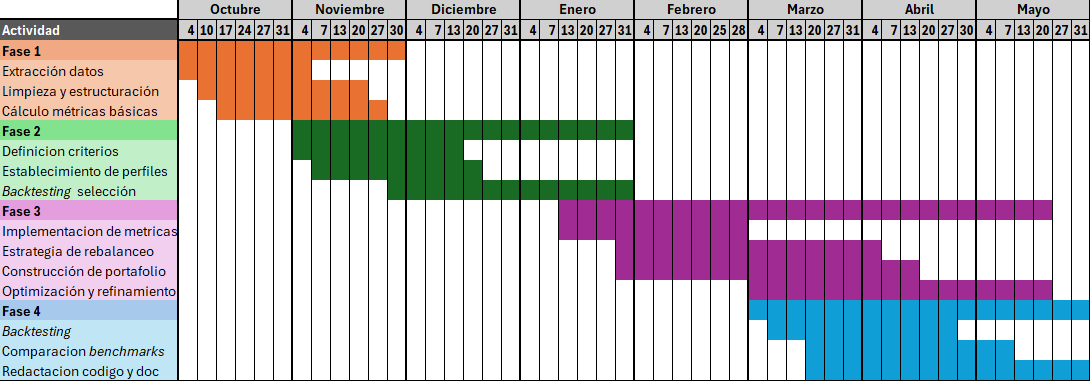
\includegraphics[width=512.930pt,height=179.250pt]{figures/figura_gantt.png}};
\node[anchor=base west,inner sep=0pt,outer sep=0pt] at ([xshift=72.000pt,yshift=-760.140pt]current page.north west) {\makebox[128.525pt][l]{{\CalibriFont\fontsize{10.02pt}{10.52pt}\selectfont\color[RGB]{0,0,0} Escuela de Ingeniería Industrial\hspace{0.25em}}}};
\node[anchor=base west,inner sep=0pt,outer sep=0pt] at ([xshift=108.020pt,yshift=-772.320pt]current page.north west) {\makebox[12.405pt][l]{{\CalibriFont\fontsize{10.02pt}{10.52pt}\selectfont\color[RGB]{0,0,0} 21\hspace{0.25em}}}};
\node[anchor=base west,inner sep=0pt,outer sep=0pt] at ([xshift=72.000pt,yshift=-85.080pt]current page.north west) {\makebox[172.355pt][l]{{\TNR\bfseries \fontsize{13.98pt}{14.68pt}\selectfont\color[RGB]{192,0,0} 5.}{\ArialFont\bfseries \fontsize{13.98pt}{14.68pt}\selectfont\color[RGB]{192,0,0} \hspace{0.25em}\hspace{0.25em}}{\TNR\bfseries \fontsize{13.98pt}{14.68pt}\selectfont\color[RGB]{192,0,0} Cronograma de Proyecto\hspace{0.25em}}}};
\node[anchor=base west,inner sep=0pt,outer sep=0pt] at ([xshift=239.060pt,yshift=-120.360pt]current page.north west) {\makebox[136.356pt][l]{{\CambriaFont\bfseries \fontsize{10.98pt}{11.53pt}\selectfont\color[RGB]{0,0,0} Figura 1}{\CambriaFont\fontsize{10.98pt}{11.53pt}\selectfont\color[RGB]{0,0,0} . Diagrama de Gantt\hspace{0.25em}}}};
\node[anchor=base west,inner sep=0pt,outer sep=0pt] at ([xshift=241.160pt,yshift=-326.180pt]current page.north west) {\makebox[132.156pt][l]{{\CambriaFont\bfseries \fontsize{10.98pt}{11.53pt}\selectfont\color[RGB]{0,0,0} Fuente.}{\CambriaFont\fontsize{10.98pt}{11.53pt}\selectfont\color[RGB]{0,0,0} \hspace{0.25em}Elaboración propia\hspace{0.25em}}}};
\node[anchor=base west,inner sep=0pt,outer sep=0pt] at ([xshift=72.000pt,yshift=-367.520pt]current page.north west) {\makebox[159.875pt][l]{{\TNR\bfseries \fontsize{13.98pt}{14.68pt}\selectfont\color[RGB]{192,0,0} 6.}{\ArialFont\bfseries \fontsize{13.98pt}{14.68pt}\selectfont\color[RGB]{192,0,0} \hspace{0.25em}\hspace{0.25em}}{\TNR\bfseries \fontsize{13.98pt}{14.68pt}\selectfont\color[RGB]{192,0,0} Alcance y Limitaciones\hspace{0.25em}}}};
\node[anchor=base west,inner sep=0pt,outer sep=0pt] at ([xshift=86.220pt,yshift=-389.840pt]current page.north west) {\makebox[456.468pt][s]{{\TNR\fontsize{12.00pt}{12.60pt}\selectfont\color[RGB]{0,0,0} El trabajo de grado se limita a un universo especifico de los activos financieros, siendo estos\hspace{0.25em}}}};
\node[anchor=base west,inner sep=0pt,outer sep=0pt] at ([xshift=72.000pt,yshift=-410.560pt]current page.north west) {\makebox[470.968pt][s]{{\TNR\fontsize{12.00pt}{12.60pt}\selectfont\color[RGB]{0,0,0} los ETFs listados y negociados en la bolsa americana en el periodo 2021-2024, por lo que solo se\hspace{0.25em}}}};
\node[anchor=base west,inner sep=0pt,outer sep=0pt] at ([xshift=72.000pt,yshift=-431.260pt]current page.north west) {\makebox[471.004pt][s]{{\TNR\fontsize{12.00pt}{12.60pt}\selectfont\color[RGB]{0,0,0} trabajaran con estos activos, el autor se ve sujeto a la disponibilidad de los datos históricos\hspace{0.25em}}}};
\node[anchor=base west,inner sep=0pt,outer sep=0pt] at ([xshift=72.000pt,yshift=-451.960pt]current page.north west) {\makebox[470.784pt][s]{{\TNR\fontsize{12.00pt}{12.60pt}\selectfont\color[RGB]{0,0,0} confiables y gratuitos a través de plataformas como Yahoo Finance, y la estandarización\hspace{0.25em}}}};
\node[anchor=base west,inner sep=0pt,outer sep=0pt] at ([xshift=72.000pt,yshift=-472.660pt]current page.north west) {\makebox[470.992pt][s]{{\TNR\fontsize{12.00pt}{12.60pt}\selectfont\color[RGB]{0,0,0} regulatoria bajo la supervisión de la\hspace{0.25em}}{\TNR\itshape \fontsize{12.00pt}{12.60pt}\selectfont\color[RGB]{0,0,0} Securities and Exchange Commission}{\TNR\fontsize{12.00pt}{12.60pt}\selectfont\color[RGB]{0,0,0} \hspace{0.25em}que garantiza\hspace{0.25em}}}};
\node[anchor=base west,inner sep=0pt,outer sep=0pt] at ([xshift=72.000pt,yshift=-493.360pt]current page.north west) {\makebox[248.560pt][l]{{\TNR\fontsize{12.00pt}{12.60pt}\selectfont\color[RGB]{0,0,0} transparencia y comparabilidad entre instrumentos.\hspace{0.25em}}}};
\node[anchor=base west,inner sep=0pt,outer sep=0pt] at ([xshift=86.220pt,yshift=-514.060pt]current page.north west) {\makebox[456.700pt][s]{{\TNR\fontsize{12.00pt}{12.60pt}\selectfont\color[RGB]{0,0,0} El horizonte temporal del estudio abarca cinco años completos desde enero de 2021 hasta\hspace{0.25em}}}};
\node[anchor=base west,inner sep=0pt,outer sep=0pt] at ([xshift=72.000pt,yshift=-534.700pt]current page.north west) {\makebox[471.060pt][s]{{\TNR\fontsize{12.00pt}{12.60pt}\selectfont\color[RGB]{0,0,0} diciembre de 2025, que aporta una estimación relevante y robusta de parámetros para el estudio,\hspace{0.25em}}}};
\node[anchor=base west,inner sep=0pt,outer sep=0pt] at ([xshift=72.000pt,yshift=-555.400pt]current page.north west) {\makebox[471.016pt][s]{{\TNR\fontsize{12.00pt}{12.60pt}\selectfont\color[RGB]{0,0,0} el periodo elegido captura múltiples etapas del mercado como la post-pandemia del 2021, la\hspace{0.25em}}}};
\node[anchor=base west,inner sep=0pt,outer sep=0pt] at ([xshift=72.000pt,yshift=-576.100pt]current page.north west) {\makebox[471.016pt][s]{{\TNR\fontsize{12.00pt}{12.60pt}\selectfont\color[RGB]{0,0,0} corrección posterior en el 2022 que represento un alza y su subsecuente estabilización en los años\hspace{0.25em}}}};
\node[anchor=base west,inner sep=0pt,outer sep=0pt] at ([xshift=72.000pt,yshift=-596.800pt]current page.north west) {\makebox[470.840pt][s]{{\TNR\fontsize{12.00pt}{12.60pt}\selectfont\color[RGB]{0,0,0} 2023 y 2024. La extensión de cinco años es suficiente para evaluar el desempeño del modelo a\hspace{0.25em}}}};
\node[anchor=base west,inner sep=0pt,outer sep=0pt] at ([xshift=72.000pt,yshift=-617.500pt]current page.north west) {\makebox[470.900pt][s]{{\TNR\fontsize{12.00pt}{12.60pt}\selectfont\color[RGB]{0,0,0} través de ciclos completos de mercado sin extenderse tanto que los datos antiguos pierdan\hspace{0.25em}}}};
\node[anchor=base west,inner sep=0pt,outer sep=0pt] at ([xshift=72.000pt,yshift=-638.200pt]current page.north west) {\makebox[236.600pt][l]{{\TNR\fontsize{12.00pt}{12.60pt}\selectfont\color[RGB]{0,0,0} relevancia para las condiciones contemporáneas.\hspace{0.25em}}}};
\PageCanvasEnd
\newpage
% -----------------------------------------------------------------------------
% Página 22
% -----------------------------------------------------------------------------
\PageCanvasStart
\path[fill={rgb,255:red,192;green,0;blue,0},draw=none] ([xshift=72.000pt,yshift=-742.195pt]current page.north west) rectangle ([xshift=600.500pt,yshift=-747.745pt]current page.north west);
\node[anchor=base west,inner sep=0pt,outer sep=0pt] at ([xshift=72.000pt,yshift=-760.140pt]current page.north west) {\makebox[128.525pt][l]{{\CalibriFont\fontsize{10.02pt}{10.52pt}\selectfont\color[RGB]{0,0,0} Escuela de Ingeniería Industrial\hspace{0.25em}}}};
\node[anchor=base west,inner sep=0pt,outer sep=0pt] at ([xshift=108.020pt,yshift=-772.320pt]current page.north west) {\makebox[12.405pt][l]{{\CalibriFont\fontsize{10.02pt}{10.52pt}\selectfont\color[RGB]{0,0,0} 22\hspace{0.25em}}}};
\node[anchor=base west,inner sep=0pt,outer sep=0pt] at ([xshift=86.220pt,yshift=-83.220pt]current page.north west) {\makebox[456.564pt][s]{{\TNR\fontsize{12.00pt}{12.60pt}\selectfont\color[RGB]{0,0,0} El modelo desarrollado está diseñado específicamente para inversionistas individuales o\hspace{0.25em}}}};
\node[anchor=base west,inner sep=0pt,outer sep=0pt] at ([xshift=72.000pt,yshift=-103.920pt]current page.north west) {\makebox[470.736pt][s]{{\TNR\fontsize{12.00pt}{12.60pt}\selectfont\color[RGB]{0,0,0} institucionales con horizontes de inversión de mediano a largo plazo, típicamente superiores a un\hspace{0.25em}}}};
\node[anchor=base west,inner sep=0pt,outer sep=0pt] at ([xshift=72.000pt,yshift=-124.620pt]current page.north west) {\makebox[470.992pt][s]{{\TNR\fontsize{12.00pt}{12.60pt}\selectfont\color[RGB]{0,0,0} año, que buscan construir portafolios diversificados de ETFs sin capacidad o interés en realizar\hspace{0.25em}}}};
\node[anchor=base west,inner sep=0pt,outer sep=0pt] at ([xshift=72.000pt,yshift=-145.340pt]current page.north west) {\makebox[470.736pt][s]{{\TNR\fontsize{12.00pt}{12.60pt}\selectfont\color[RGB]{0,0,0} trading activo de alta frecuencia. El perfil de usuario objetivo incluye inversionistas con capital\hspace{0.25em}}}};
\node[anchor=base west,inner sep=0pt,outer sep=0pt] at ([xshift=72.000pt,yshift=-166.040pt]current page.north west) {\makebox[470.736pt][s]{{\TNR\fontsize{12.00pt}{12.60pt}\selectfont\color[RGB]{0,0,0} suficiente para mantener posiciones en diez a veinte ETFs diferentes sin que los costos fijos de\hspace{0.25em}}}};
\node[anchor=base west,inner sep=0pt,outer sep=0pt] at ([xshift=72.000pt,yshift=-186.740pt]current page.north west) {\makebox[338.200pt][l]{{\TNR\fontsize{12.00pt}{12.60pt}\selectfont\color[RGB]{0,0,0} transacción representen una proporción excesiva del capital invertido.\hspace{0.25em}}}};
\node[anchor=base west,inner sep=0pt,outer sep=0pt] at ([xshift=86.220pt,yshift=-207.440pt]current page.north west) {\makebox[456.552pt][s]{{\TNR\fontsize{12.00pt}{12.60pt}\selectfont\color[RGB]{0,0,0} El alcance del modelo resultante solo contempla posiciones largas, otras operaciones como\hspace{0.25em}}}};
\node[anchor=base west,inner sep=0pt,outer sep=0pt] at ([xshift=72.000pt,yshift=-228.140pt]current page.north west) {\makebox[470.736pt][s]{{\TNR\fontsize{12.00pt}{12.60pt}\selectfont\color[RGB]{0,0,0} ventas en corto o opciones no se tienen en cuenta, pues es desde la perspectiva de un inversor\hspace{0.25em}}}};
\node[anchor=base west,inner sep=0pt,outer sep=0pt] at ([xshift=72.000pt,yshift=-248.840pt]current page.north west) {\makebox[183.380pt][l]{{\TNR\fontsize{12.00pt}{12.60pt}\selectfont\color[RGB]{0,0,0} individual con un portafolio ajustado.\hspace{0.25em}}}};
\PageCanvasEnd
\newpage
% -----------------------------------------------------------------------------
% Página 23
% -----------------------------------------------------------------------------
\PageCanvasStart
\path[fill={rgb,255:red,192;green,0;blue,0},draw=none] ([xshift=72.000pt,yshift=-742.195pt]current page.north west) rectangle ([xshift=600.500pt,yshift=-747.745pt]current page.north west);
\path[fill={rgb,255:red,0;green,0;blue,0},draw=none] ([xshift=103.520pt,yshift=-328.940pt]current page.north west) rectangle ([xshift=297.020pt,yshift=-329.420pt]current page.north west);
\path[fill={rgb,255:red,0;green,0;blue,0},draw=none] ([xshift=297.020pt,yshift=-328.940pt]current page.north west) rectangle ([xshift=297.500pt,yshift=-329.420pt]current page.north west);
\path[fill={rgb,255:red,0;green,0;blue,0},draw=none] ([xshift=297.500pt,yshift=-328.940pt]current page.north west) rectangle ([xshift=508.540pt,yshift=-329.420pt]current page.north west);
\path[fill={rgb,255:red,0;green,0;blue,0},draw=none] ([xshift=103.520pt,yshift=-346.700pt]current page.north west) rectangle ([xshift=297.020pt,yshift=-347.180pt]current page.north west);
\path[fill={rgb,255:red,0;green,0;blue,0},draw=none] ([xshift=297.020pt,yshift=-346.700pt]current page.north west) rectangle ([xshift=297.500pt,yshift=-347.180pt]current page.north west);
\path[fill={rgb,255:red,0;green,0;blue,0},draw=none] ([xshift=297.500pt,yshift=-346.700pt]current page.north west) rectangle ([xshift=508.540pt,yshift=-347.180pt]current page.north west);
\path[fill={rgb,255:red,0;green,0;blue,0},draw=none] ([xshift=102.800pt,yshift=-485.200pt]current page.north west) rectangle ([xshift=297.020pt,yshift=-485.680pt]current page.north west);
\path[fill={rgb,255:red,0;green,0;blue,0},draw=none] ([xshift=296.300pt,yshift=-485.200pt]current page.north west) rectangle ([xshift=296.780pt,yshift=-485.680pt]current page.north west);
\path[fill={rgb,255:red,0;green,0;blue,0},draw=none] ([xshift=296.780pt,yshift=-485.200pt]current page.north west) rectangle ([xshift=508.540pt,yshift=-485.680pt]current page.north west);
\node[anchor=base west,inner sep=0pt,outer sep=0pt] at ([xshift=72.000pt,yshift=-760.140pt]current page.north west) {\makebox[128.525pt][l]{{\CalibriFont\fontsize{10.02pt}{10.52pt}\selectfont\color[RGB]{0,0,0} Escuela de Ingeniería Industrial\hspace{0.25em}}}};
\node[anchor=base west,inner sep=0pt,outer sep=0pt] at ([xshift=108.020pt,yshift=-772.320pt]current page.north west) {\makebox[12.405pt][l]{{\CalibriFont\fontsize{10.02pt}{10.52pt}\selectfont\color[RGB]{0,0,0} 23\hspace{0.25em}}}};
\node[anchor=base west,inner sep=0pt,outer sep=0pt] at ([xshift=72.000pt,yshift=-85.080pt]current page.north west) {\makebox[369.595pt][l]{{\TNR\bfseries \fontsize{13.98pt}{14.68pt}\selectfont\color[RGB]{192,0,0} 7.}{\ArialFont\bfseries \fontsize{13.98pt}{14.68pt}\selectfont\color[RGB]{192,0,0} \hspace{0.25em}\hspace{0.25em}}{\TNR\bfseries \fontsize{13.98pt}{14.68pt}\selectfont\color[RGB]{192,0,0} Implementación del Sistema de Clasificación Multicriterio\hspace{0.25em}}}};
\node[anchor=base west,inner sep=0pt,outer sep=0pt] at ([xshift=86.220pt,yshift=-107.340pt]current page.north west) {\makebox[456.656pt][s]{{\TNR\fontsize{12.00pt}{12.60pt}\selectfont\color[RGB]{0,0,0} El desarrollo del sistema de clasificación multicriterio mediante ELECTRE Tri constituye el\hspace{0.25em}}}};
\node[anchor=base west,inner sep=0pt,outer sep=0pt] at ([xshift=72.000pt,yshift=-128.040pt]current page.north west) {\makebox[470.828pt][s]{{\TNR\fontsize{12.00pt}{12.60pt}\selectfont\color[RGB]{0,0,0} centro metodológico del primer objetivo específico de esta investigación. La implementación se\hspace{0.25em}}}};
\node[anchor=base west,inner sep=0pt,outer sep=0pt] at ([xshift=72.000pt,yshift=-148.760pt]current page.north west) {\makebox[471.060pt][s]{{\TNR\fontsize{12.00pt}{12.60pt}\selectfont\color[RGB]{0,0,0} fundamenta en la adaptación de la metodología propuesta por Xidonas et al. (2009) al mercado\hspace{0.25em}}}};
\node[anchor=base west,inner sep=0pt,outer sep=0pt] at ([xshift=72.000pt,yshift=-169.460pt]current page.north west) {\makebox[471.060pt][s]{{\TNR\fontsize{12.00pt}{12.60pt}\selectfont\color[RGB]{0,0,0} específico de\hspace{0.25em}}{\TNR\itshape \fontsize{12.00pt}{12.60pt}\selectfont\color[RGB]{0,0,0} Exchange-Traded Funds (ETFs),}{\TNR\fontsize{12.00pt}{12.60pt}\selectfont\color[RGB]{0,0,0} \hspace{0.25em}considerando las particularidades e idiosincrasias\hspace{0.25em}}}};
\node[anchor=base west,inner sep=0pt,outer sep=0pt] at ([xshift=72.000pt,yshift=-190.160pt]current page.north west) {\makebox[470.748pt][s]{{\TNR\fontsize{12.00pt}{12.60pt}\selectfont\color[RGB]{0,0,0} estructurales y operativas de estos instrumentos financieros que los diferencian de las acciones\hspace{0.25em}}}};
\node[anchor=base west,inner sep=0pt,outer sep=0pt] at ([xshift=72.000pt,yshift=-210.860pt]current page.north west) {\makebox[314.560pt][l]{{\TNR\fontsize{12.00pt}{12.60pt}\selectfont\color[RGB]{0,0,0} individuales tradicionalmente analizadas en la literatura MCDM.\hspace{0.25em}}}};
\node[anchor=base west,inner sep=0pt,outer sep=0pt] at ([xshift=86.220pt,yshift=-252.260pt]current page.north west) {\makebox[456.684pt][s]{{\TNR\fontsize{12.00pt}{12.60pt}\selectfont\color[RGB]{0,0,0} La arquitectura del sistema se estructura en torno a seis criterios de evaluación cuidadosamente\hspace{0.25em}}}};
\node[anchor=base west,inner sep=0pt,outer sep=0pt] at ([xshift=72.000pt,yshift=-272.960pt]current page.north west) {\makebox[427.180pt][s]{{\TNR\fontsize{12.00pt}{12.60pt}\selectfont\color[RGB]{0,0,0} seleccionados para capturar las dimensiones más relevantes del desempeño de los ETFs:\hspace{0.25em}}}};
\node[anchor=base west,inner sep=0pt,outer sep=0pt] at ([xshift=226.880pt,yshift=-319.460pt]current page.north west) {\makebox[161.300pt][l]{{\TNR\bfseries \fontsize{12.00pt}{12.60pt}\selectfont\color[RGB]{0,0,0} Tabla 2.}{\TNR\fontsize{12.00pt}{12.60pt}\selectfont\color[RGB]{0,0,0} \hspace{0.25em}Criterios de Evaluación\hspace{0.25em}}}};
\node[anchor=base west,inner sep=0pt,outer sep=0pt] at ([xshift=153.020pt,yshift=-338.780pt]current page.north west) {\makebox[96.945pt][l]{{\TNR\fontsize{10.02pt}{10.52pt}\selectfont\color[RGB]{0,0,0} Criterios de Evaluación\hspace{0.25em}}}};
\node[anchor=base west,inner sep=0pt,outer sep=0pt] at ([xshift=393.280pt,yshift=-338.780pt]current page.north west) {\makebox[21.405pt][l]{{\TNR\fontsize{10.02pt}{10.52pt}\selectfont\color[RGB]{0,0,0} Peso\hspace{0.25em}}}};
\node[anchor=base west,inner sep=0pt,outer sep=0pt] at ([xshift=135.080pt,yshift=-373.820pt]current page.north west) {\makebox[132.765pt][l]{{\TNR\fontsize{10.02pt}{10.52pt}\selectfont\color[RGB]{0,0,0} Compound Annual Growth Rate\hspace{0.25em}}}};
\node[anchor=base west,inner sep=0pt,outer sep=0pt] at ([xshift=174.260pt,yshift=-391.040pt]current page.north west) {\makebox[54.465pt][l]{{\TNR\fontsize{10.02pt}{10.52pt}\selectfont\color[RGB]{0,0,0} Sharpe Ratio\hspace{0.25em}}}};
\node[anchor=base west,inner sep=0pt,outer sep=0pt] at ([xshift=153.740pt,yshift=-408.320pt]current page.north west) {\makebox[95.505pt][l]{{\TNR\fontsize{10.02pt}{10.52pt}\selectfont\color[RGB]{0,0,0} Volatilidad Anualizada\hspace{0.25em}}}};
\node[anchor=base west,inner sep=0pt,outer sep=0pt] at ([xshift=182.480pt,yshift=-425.560pt]current page.north west) {\makebox[38.025pt][l]{{\TNR\fontsize{10.02pt}{10.52pt}\selectfont\color[RGB]{0,0,0} Liquidez\hspace{0.25em}}}};
\node[anchor=base west,inner sep=0pt,outer sep=0pt] at ([xshift=170.360pt,yshift=-442.840pt]current page.north west) {\makebox[62.205pt][l]{{\TNR\fontsize{10.02pt}{10.52pt}\selectfont\color[RGB]{0,0,0} Tracking Error\hspace{0.25em}}}};
\node[anchor=base west,inner sep=0pt,outer sep=0pt] at ([xshift=172.880pt,yshift=-460.060pt]current page.north west) {\makebox[57.225pt][l]{{\TNR\fontsize{10.02pt}{10.52pt}\selectfont\color[RGB]{0,0,0} Expense ratio\hspace{0.25em}}}};
\node[anchor=base west,inner sep=0pt,outer sep=0pt] at ([xshift=393.580pt,yshift=-373.820pt]current page.north west) {\makebox[20.805pt][l]{{\TNR\fontsize{10.02pt}{10.52pt}\selectfont\color[RGB]{0,0,0} 25\%\hspace{0.25em}}}};
\node[anchor=base west,inner sep=0pt,outer sep=0pt] at ([xshift=393.580pt,yshift=-391.040pt]current page.north west) {\makebox[20.805pt][l]{{\TNR\fontsize{10.02pt}{10.52pt}\selectfont\color[RGB]{0,0,0} 20\%\hspace{0.25em}}}};
\node[anchor=base west,inner sep=0pt,outer sep=0pt] at ([xshift=393.580pt,yshift=-408.320pt]current page.north west) {\makebox[20.805pt][l]{{\TNR\fontsize{10.02pt}{10.52pt}\selectfont\color[RGB]{0,0,0} 15\%\hspace{0.25em}}}};
\node[anchor=base west,inner sep=0pt,outer sep=0pt] at ([xshift=393.580pt,yshift=-425.560pt]current page.north west) {\makebox[20.805pt][l]{{\TNR\fontsize{10.02pt}{10.52pt}\selectfont\color[RGB]{0,0,0} 15\%\hspace{0.25em}}}};
\node[anchor=base west,inner sep=0pt,outer sep=0pt] at ([xshift=393.580pt,yshift=-442.840pt]current page.north west) {\makebox[20.805pt][l]{{\TNR\fontsize{10.02pt}{10.52pt}\selectfont\color[RGB]{0,0,0} 15\%\hspace{0.25em}}}};
\node[anchor=base west,inner sep=0pt,outer sep=0pt] at ([xshift=393.580pt,yshift=-460.060pt]current page.north west) {\makebox[20.805pt][l]{{\TNR\fontsize{10.02pt}{10.52pt}\selectfont\color[RGB]{0,0,0} 10\%\hspace{0.25em}}}};
\node[anchor=base west,inner sep=0pt,outer sep=0pt] at ([xshift=224.360pt,yshift=-496.900pt]current page.north west) {\makebox[166.280pt][l]{{\TNR\fontsize{12.00pt}{12.60pt}\selectfont\color[RGB]{0,0,0} Fuente: construido por los autores\hspace{0.25em}}}};
\node[anchor=base west,inner sep=0pt,outer sep=0pt] at ([xshift=86.220pt,yshift=-545.200pt]current page.north west) {\makebox[456.576pt][s]{{\TNR\fontsize{12.00pt}{12.60pt}\selectfont\color[RGB]{0,0,0} Esta ponderación refleja la jerarquía de importancia establecida en la literatura especializada,\hspace{0.25em}}}};
\node[anchor=base west,inner sep=0pt,outer sep=0pt] at ([xshift=72.000pt,yshift=-565.900pt]current page.north west) {\makebox[470.736pt][s]{{\TNR\fontsize{12.00pt}{12.60pt}\selectfont\color[RGB]{0,0,0} donde el rendimiento y la eficiencia de riesgo mantienen la mayor relevancia para la toma de\hspace{0.25em}}}};
\node[anchor=base west,inner sep=0pt,outer sep=0pt] at ([xshift=72.000pt,yshift=-586.600pt]current page.north west) {\makebox[117.980pt][l]{{\TNR\fontsize{12.00pt}{12.60pt}\selectfont\color[RGB]{0,0,0} decisiones de inversión.\hspace{0.25em}}}};
\node[anchor=base west,inner sep=0pt,outer sep=0pt] at ([xshift=72.000pt,yshift=-625.000pt]current page.north west) {\makebox[345.235pt][l]{{\TNR\bfseries \fontsize{13.98pt}{14.68pt}\selectfont\color[RGB]{192,0,0} 7.1. Definición de Categorías y Umbrales de Clasificación\hspace{0.25em}}}};
\node[anchor=base west,inner sep=0pt,outer sep=0pt] at ([xshift=72.000pt,yshift=-665.020pt]current page.north west) {\makebox[470.736pt][s]{{\TNR\fontsize{12.00pt}{12.60pt}\selectfont\color[RGB]{0,0,0} Se siguen los lineamientos de la metodología ELECTRE Tri donde se determinan a priori\hspace{0.25em}}}};
\node[anchor=base west,inner sep=0pt,outer sep=0pt] at ([xshift=72.000pt,yshift=-685.720pt]current page.north west) {\makebox[470.724pt][s]{{\TNR\fontsize{12.00pt}{12.60pt}\selectfont\color[RGB]{0,0,0} categorías de clasificación, en este caso se establecieron tres categorías ordenadas que reflejan la\hspace{0.25em}}}};
\node[anchor=base west,inner sep=0pt,outer sep=0pt] at ([xshift=72.000pt,yshift=-706.440pt]current page.north west) {\makebox[471.060pt][s]{{\TNR\fontsize{12.00pt}{12.60pt}\selectfont\color[RGB]{0,0,0} calidad relativa de los ETFs en el universo de análisis: "Excelentes", "Aceptables" y "Rechazados".\hspace{0.25em}}}};
\PageCanvasEnd
\newpage
% -----------------------------------------------------------------------------
% Página 24
% -----------------------------------------------------------------------------
\PageCanvasStart
\path[fill={rgb,255:red,192;green,0;blue,0},draw=none] ([xshift=72.000pt,yshift=-742.195pt]current page.north west) rectangle ([xshift=600.500pt,yshift=-747.745pt]current page.north west);
\path[fill={rgb,255:red,0;green,0;blue,0},draw=none] ([xshift=159.080pt,yshift=-166.820pt]current page.north west) rectangle ([xshift=296.360pt,yshift=-167.300pt]current page.north west);
\path[fill={rgb,255:red,0;green,0;blue,0},draw=none] ([xshift=296.360pt,yshift=-166.820pt]current page.north west) rectangle ([xshift=296.840pt,yshift=-167.300pt]current page.north west);
\path[fill={rgb,255:red,0;green,0;blue,0},draw=none] ([xshift=296.840pt,yshift=-166.820pt]current page.north west) rectangle ([xshift=346.780pt,yshift=-167.300pt]current page.north west);
\path[fill={rgb,255:red,0;green,0;blue,0},draw=none] ([xshift=346.780pt,yshift=-166.820pt]current page.north west) rectangle ([xshift=347.260pt,yshift=-167.300pt]current page.north west);
\path[fill={rgb,255:red,0;green,0;blue,0},draw=none] ([xshift=347.260pt,yshift=-166.820pt]current page.north west) rectangle ([xshift=398.200pt,yshift=-167.300pt]current page.north west);
\path[fill={rgb,255:red,0;green,0;blue,0},draw=none] ([xshift=398.200pt,yshift=-166.820pt]current page.north west) rectangle ([xshift=398.680pt,yshift=-167.300pt]current page.north west);
\path[fill={rgb,255:red,0;green,0;blue,0},draw=none] ([xshift=398.680pt,yshift=-166.820pt]current page.north west) rectangle ([xshift=452.980pt,yshift=-167.300pt]current page.north west);
\path[fill={rgb,255:red,0;green,0;blue,0},draw=none] ([xshift=159.080pt,yshift=-184.580pt]current page.north west) rectangle ([xshift=296.360pt,yshift=-185.060pt]current page.north west);
\path[fill={rgb,255:red,0;green,0;blue,0},draw=none] ([xshift=296.360pt,yshift=-184.580pt]current page.north west) rectangle ([xshift=296.840pt,yshift=-185.060pt]current page.north west);
\path[fill={rgb,255:red,0;green,0;blue,0},draw=none] ([xshift=296.840pt,yshift=-184.580pt]current page.north west) rectangle ([xshift=346.780pt,yshift=-185.060pt]current page.north west);
\path[fill={rgb,255:red,0;green,0;blue,0},draw=none] ([xshift=346.780pt,yshift=-184.580pt]current page.north west) rectangle ([xshift=347.260pt,yshift=-185.060pt]current page.north west);
\path[fill={rgb,255:red,0;green,0;blue,0},draw=none] ([xshift=347.260pt,yshift=-184.580pt]current page.north west) rectangle ([xshift=398.200pt,yshift=-185.060pt]current page.north west);
\path[fill={rgb,255:red,0;green,0;blue,0},draw=none] ([xshift=398.200pt,yshift=-184.580pt]current page.north west) rectangle ([xshift=398.680pt,yshift=-185.060pt]current page.north west);
\path[fill={rgb,255:red,0;green,0;blue,0},draw=none] ([xshift=398.680pt,yshift=-184.580pt]current page.north west) rectangle ([xshift=452.980pt,yshift=-185.060pt]current page.north west);
\path[fill={rgb,255:red,0;green,0;blue,0},draw=none] ([xshift=158.360pt,yshift=-323.060pt]current page.north west) rectangle ([xshift=296.360pt,yshift=-323.540pt]current page.north west);
\path[fill={rgb,255:red,0;green,0;blue,0},draw=none] ([xshift=295.640pt,yshift=-323.060pt]current page.north west) rectangle ([xshift=296.120pt,yshift=-323.540pt]current page.north west);
\path[fill={rgb,255:red,0;green,0;blue,0},draw=none] ([xshift=296.120pt,yshift=-323.060pt]current page.north west) rectangle ([xshift=346.780pt,yshift=-323.540pt]current page.north west);
\path[fill={rgb,255:red,0;green,0;blue,0},draw=none] ([xshift=346.060pt,yshift=-323.060pt]current page.north west) rectangle ([xshift=346.540pt,yshift=-323.540pt]current page.north west);
\path[fill={rgb,255:red,0;green,0;blue,0},draw=none] ([xshift=346.540pt,yshift=-323.060pt]current page.north west) rectangle ([xshift=398.200pt,yshift=-323.540pt]current page.north west);
\path[fill={rgb,255:red,0;green,0;blue,0},draw=none] ([xshift=397.480pt,yshift=-323.060pt]current page.north west) rectangle ([xshift=397.960pt,yshift=-323.540pt]current page.north west);
\path[fill={rgb,255:red,0;green,0;blue,0},draw=none] ([xshift=397.960pt,yshift=-323.060pt]current page.north west) rectangle ([xshift=452.980pt,yshift=-323.540pt]current page.north west);
\node[anchor=base west,inner sep=0pt,outer sep=0pt] at ([xshift=72.000pt,yshift=-760.140pt]current page.north west) {\makebox[128.525pt][l]{{\CalibriFont\fontsize{10.02pt}{10.52pt}\selectfont\color[RGB]{0,0,0} Escuela de Ingeniería Industrial\hspace{0.25em}}}};
\node[anchor=base west,inner sep=0pt,outer sep=0pt] at ([xshift=108.020pt,yshift=-772.320pt]current page.north west) {\makebox[12.405pt][l]{{\CalibriFont\fontsize{10.02pt}{10.52pt}\selectfont\color[RGB]{0,0,0} 24\hspace{0.25em}}}};
\node[anchor=base west,inner sep=0pt,outer sep=0pt] at ([xshift=72.000pt,yshift=-83.220pt]current page.north west) {\makebox[471.040pt][s]{{\TNR\fontsize{12.00pt}{12.60pt}\selectfont\color[RGB]{0,0,0} Estas categorías vienen definidas en el método expuesto en el trabajo de Xidonas et al, los umbrales\hspace{0.25em}}}};
\node[anchor=base west,inner sep=0pt,outer sep=0pt] at ([xshift=72.000pt,yshift=-103.920pt]current page.north west) {\makebox[470.968pt][s]{{\TNR\fontsize{12.00pt}{12.60pt}\selectfont\color[RGB]{0,0,0} que determinan a que categoría pertenece cada activo se definen en el código de la siguiente\hspace{0.25em}}}};
\node[anchor=base west,inner sep=0pt,outer sep=0pt] at ([xshift=72.000pt,yshift=-124.620pt]current page.north west) {\makebox[41.300pt][l]{{\TNR\fontsize{12.00pt}{12.60pt}\selectfont\color[RGB]{0,0,0} manera.\hspace{0.25em}}}};
\node[anchor=base west,inner sep=0pt,outer sep=0pt] at ([xshift=227.000pt,yshift=-157.340pt]current page.north west) {\makebox[161.000pt][l]{{\TNR\fontsize{12.00pt}{12.60pt}\selectfont\color[RGB]{0,0,0} \hspace{0.25em}\hspace{0.25em}}{\TNR\bfseries \fontsize{12.00pt}{12.60pt}\selectfont\color[RGB]{0,0,0} Tabla 3.}{\TNR\fontsize{12.00pt}{12.60pt}\selectfont\color[RGB]{0,0,0} \hspace{0.25em}Categorías y Umbrales\hspace{0.25em}}}};
\node[anchor=base west,inner sep=0pt,outer sep=0pt] at ([xshift=180.500pt,yshift=-176.660pt]current page.north west) {\makebox[96.945pt][l]{{\TNR\fontsize{10.02pt}{10.52pt}\selectfont\color[RGB]{0,0,0} Criterios de Evaluación\hspace{0.25em}}}};
\node[anchor=base west,inner sep=0pt,outer sep=0pt] at ([xshift=299.900pt,yshift=-176.660pt]current page.north west) {\makebox[152.045pt][l]{{\TNR\fontsize{10.02pt}{10.52pt}\selectfont\color[RGB]{0,0,0} Excelentes Aceptables Rechazados\hspace{0.25em}}}};
\node[anchor=base west,inner sep=0pt,outer sep=0pt] at ([xshift=162.560pt,yshift=-211.700pt]current page.north west) {\makebox[132.765pt][l]{{\TNR\fontsize{10.02pt}{10.52pt}\selectfont\color[RGB]{0,0,0} Compound Annual Growth Rate\hspace{0.25em}}}};
\node[anchor=base west,inner sep=0pt,outer sep=0pt] at ([xshift=201.740pt,yshift=-228.920pt]current page.north west) {\makebox[54.465pt][l]{{\TNR\fontsize{10.02pt}{10.52pt}\selectfont\color[RGB]{0,0,0} Sharpe Ratio\hspace{0.25em}}}};
\node[anchor=base west,inner sep=0pt,outer sep=0pt] at ([xshift=181.220pt,yshift=-246.140pt]current page.north west) {\makebox[95.505pt][l]{{\TNR\fontsize{10.02pt}{10.52pt}\selectfont\color[RGB]{0,0,0} Volatilidad Anualizada\hspace{0.25em}}}};
\node[anchor=base west,inner sep=0pt,outer sep=0pt] at ([xshift=209.960pt,yshift=-263.420pt]current page.north west) {\makebox[38.025pt][l]{{\TNR\fontsize{10.02pt}{10.52pt}\selectfont\color[RGB]{0,0,0} Liquidez\hspace{0.25em}}}};
\node[anchor=base west,inner sep=0pt,outer sep=0pt] at ([xshift=197.840pt,yshift=-280.640pt]current page.north west) {\makebox[62.205pt][l]{{\TNR\fontsize{10.02pt}{10.52pt}\selectfont\color[RGB]{0,0,0} Tracking Error\hspace{0.25em}}}};
\node[anchor=base west,inner sep=0pt,outer sep=0pt] at ([xshift=200.360pt,yshift=-297.920pt]current page.north west) {\makebox[57.225pt][l]{{\TNR\fontsize{10.02pt}{10.52pt}\selectfont\color[RGB]{0,0,0} Expense ratio\hspace{0.25em}}}};
\node[anchor=base west,inner sep=0pt,outer sep=0pt] at ([xshift=312.080pt,yshift=-211.700pt]current page.north west) {\makebox[21.485pt][l]{{\TNR\fontsize{10.02pt}{10.52pt}\selectfont\color[RGB]{0,0,0} 8\%>\hspace{0.25em}}}};
\node[anchor=base west,inner sep=0pt,outer sep=0pt] at ([xshift=312.500pt,yshift=-228.920pt]current page.north west) {\makebox[20.645pt][l]{{\TNR\fontsize{10.02pt}{10.52pt}\selectfont\color[RGB]{0,0,0} 0.8>\hspace{0.25em}}}};
\node[anchor=base west,inner sep=0pt,outer sep=0pt] at ([xshift=362.980pt,yshift=-211.700pt]current page.north west) {\makebox[21.465pt][l]{{\TNR\fontsize{10.02pt}{10.52pt}\selectfont\color[RGB]{0,0,0} 5\%>\hspace{0.25em}}}};
\node[anchor=base west,inner sep=0pt,outer sep=0pt] at ([xshift=363.400pt,yshift=-228.920pt]current page.north west) {\makebox[20.625pt][l]{{\TNR\fontsize{10.02pt}{10.52pt}\selectfont\color[RGB]{0,0,0} 0.4>\hspace{0.25em}}}};
\node[anchor=base west,inner sep=0pt,outer sep=0pt] at ([xshift=416.080pt,yshift=-211.700pt]current page.north west) {\makebox[21.465pt][l]{{\TNR\fontsize{10.02pt}{10.52pt}\selectfont\color[RGB]{0,0,0} >5\%\hspace{0.25em}}}};
\node[anchor=base west,inner sep=0pt,outer sep=0pt] at ([xshift=416.500pt,yshift=-228.920pt]current page.north west) {\makebox[20.625pt][l]{{\TNR\fontsize{10.02pt}{10.52pt}\selectfont\color[RGB]{0,0,0} >0.2\hspace{0.25em}}}};
\node[anchor=base west,inner sep=0pt,outer sep=0pt] at ([xshift=309.620pt,yshift=-246.140pt]current page.north west) {\makebox[26.465pt][l]{{\TNR\fontsize{10.02pt}{10.52pt}\selectfont\color[RGB]{0,0,0} >25\%\hspace{0.25em}}}};
\node[anchor=base west,inner sep=0pt,outer sep=0pt] at ([xshift=360.520pt,yshift=-246.140pt]current page.north west) {\makebox[26.445pt][l]{{\TNR\fontsize{10.02pt}{10.52pt}\selectfont\color[RGB]{0,0,0} >35\%\hspace{0.25em}}}};
\node[anchor=base west,inner sep=0pt,outer sep=0pt] at ([xshift=413.620pt,yshift=-246.140pt]current page.north west) {\makebox[26.445pt][l]{{\TNR\fontsize{10.02pt}{10.52pt}\selectfont\color[RGB]{0,0,0} 50\%>\hspace{0.25em}}}};
\node[anchor=base west,inner sep=0pt,outer sep=0pt] at ([xshift=312.500pt,yshift=-263.420pt]current page.north west) {\makebox[20.645pt][l]{{\TNR\fontsize{10.02pt}{10.52pt}\selectfont\color[RGB]{0,0,0} 0.6>\hspace{0.25em}}}};
\node[anchor=base west,inner sep=0pt,outer sep=0pt] at ([xshift=312.080pt,yshift=-280.640pt]current page.north west) {\makebox[21.485pt][l]{{\TNR\fontsize{10.02pt}{10.52pt}\selectfont\color[RGB]{0,0,0} >6\%\hspace{0.25em}}}};
\node[anchor=base west,inner sep=0pt,outer sep=0pt] at ([xshift=312.080pt,yshift=-297.920pt]current page.north west) {\makebox[21.485pt][l]{{\TNR\fontsize{10.02pt}{10.52pt}\selectfont\color[RGB]{0,0,0} >2\%\hspace{0.25em}}}};
\node[anchor=base west,inner sep=0pt,outer sep=0pt] at ([xshift=363.400pt,yshift=-263.420pt]current page.north west) {\makebox[20.625pt][l]{{\TNR\fontsize{10.02pt}{10.52pt}\selectfont\color[RGB]{0,0,0} 0.4>\hspace{0.25em}}}};
\node[anchor=base west,inner sep=0pt,outer sep=0pt] at ([xshift=362.980pt,yshift=-280.640pt]current page.north west) {\makebox[21.465pt][l]{{\TNR\fontsize{10.02pt}{10.52pt}\selectfont\color[RGB]{0,0,0} >8\%\hspace{0.25em}}}};
\node[anchor=base west,inner sep=0pt,outer sep=0pt] at ([xshift=362.980pt,yshift=-297.920pt]current page.north west) {\makebox[21.465pt][l]{{\TNR\fontsize{10.02pt}{10.52pt}\selectfont\color[RGB]{0,0,0} >3\%\hspace{0.25em}}}};
\node[anchor=base west,inner sep=0pt,outer sep=0pt] at ([xshift=416.500pt,yshift=-263.420pt]current page.north west) {\makebox[20.625pt][l]{{\TNR\fontsize{10.02pt}{10.52pt}\selectfont\color[RGB]{0,0,0} >0.2\hspace{0.25em}}}};
\node[anchor=base west,inner sep=0pt,outer sep=0pt] at ([xshift=413.620pt,yshift=-280.640pt]current page.north west) {\makebox[26.445pt][l]{{\TNR\fontsize{10.02pt}{10.52pt}\selectfont\color[RGB]{0,0,0} 15\%>\hspace{0.25em}}}};
\node[anchor=base west,inner sep=0pt,outer sep=0pt] at ([xshift=416.080pt,yshift=-297.920pt]current page.north west) {\makebox[21.210pt][l]{{\TNR\fontsize{10.02pt}{10.52pt}\selectfont\color[RGB]{0,0,0} 5\%>}{\TNR\fontsize{9.00pt}{9.45pt}\selectfont\color[RGB]{0,0,0} \hspace{0.25em}\hspace{0.25em}}}};
\node[anchor=base west,inner sep=0pt,outer sep=0pt] at ([xshift=224.360pt,yshift=-334.760pt]current page.north west) {\makebox[166.280pt][l]{{\TNR\fontsize{12.00pt}{12.60pt}\selectfont\color[RGB]{0,0,0} Fuente: construido por los autores\hspace{0.25em}}}};
\node[anchor=base west,inner sep=0pt,outer sep=0pt] at ([xshift=86.220pt,yshift=-389.960pt]current page.north west) {\makebox[456.820pt][s]{{\TNR\fontsize{12.00pt}{12.60pt}\selectfont\color[RGB]{0,0,0} Se implementó el sistema ELECTRE Tri a través de Python utilizando las librerías\hspace{0.25em}}{\TNR\itshape \fontsize{12.00pt}{12.60pt}\selectfont\color[RGB]{0,0,0} numpy,\hspace{0.25em}}}};
\node[anchor=base west,inner sep=0pt,outer sep=0pt] at ([xshift=72.000pt,yshift=-410.680pt]current page.north west) {\makebox[470.876pt][s]{{\TNR\itshape \fontsize{12.00pt}{12.60pt}\selectfont\color[RGB]{0,0,0} pandas\hspace{0.25em}}{\TNR\fontsize{12.00pt}{12.60pt}\selectfont\color[RGB]{0,0,0} y}{\TNR\itshape \fontsize{12.00pt}{12.60pt}\selectfont\color[RGB]{0,0,0} \hspace{0.25em}scipy}{\TNR\fontsize{12.00pt}{12.60pt}\selectfont\color[RGB]{0,0,0} , garantizando tanto la eficiencia computacional como la replicabilidad de los\hspace{0.25em}}}};
\node[anchor=base west,inner sep=0pt,outer sep=0pt] at ([xshift=72.000pt,yshift=-431.380pt]current page.north west) {\makebox[470.932pt][s]{{\TNR\fontsize{12.00pt}{12.60pt}\selectfont\color[RGB]{0,0,0} resultados a través de su publicación libre por medio de GitHub. El algoritmo implementa los\hspace{0.25em}}}};
\node[anchor=base west,inner sep=0pt,outer sep=0pt] at ([xshift=72.000pt,yshift=-452.080pt]current page.north west) {\makebox[470.784pt][s]{{\TNR\fontsize{12.00pt}{12.60pt}\selectfont\color[RGB]{0,0,0} procedimientos de asignación pesimista y optimista característicos de ELECTRE Tri, calculando\hspace{0.25em}}}};
\node[anchor=base west,inner sep=0pt,outer sep=0pt] at ([xshift=72.000pt,yshift=-472.780pt]current page.north west) {\makebox[470.760pt][s]{{\TNR\fontsize{12.00pt}{12.60pt}\selectfont\color[RGB]{0,0,0} índices de concordancia y discordancia para cada alternativa respecto a los perfiles de referencia,\hspace{0.25em}}}};
\node[anchor=base west,inner sep=0pt,outer sep=0pt] at ([xshift=72.000pt,yshift=-493.480pt]current page.north west) {\makebox[352.360pt][l]{{\TNR\fontsize{12.00pt}{12.60pt}\selectfont\color[RGB]{0,0,0} y derivando índices de credibilidad que determinan la clasificación final.\hspace{0.25em}}}};
\node[anchor=base west,inner sep=0pt,outer sep=0pt] at ([xshift=86.220pt,yshift=-534.880pt]current page.north west) {\makebox[456.808pt][s]{{\TNR\fontsize{12.00pt}{12.60pt}\selectfont\color[RGB]{0,0,0} Los umbrales de indiferencia, preferencia y veto se determinaron a través de análisis estadístico\hspace{0.25em}}}};
\node[anchor=base west,inner sep=0pt,outer sep=0pt] at ([xshift=72.000pt,yshift=-555.580pt]current page.north west) {\makebox[470.916pt][s]{{\TNR\fontsize{12.00pt}{12.60pt}\selectfont\color[RGB]{0,0,0} del universo de ETFs, estableciendo valores que reflejan la variabilidad natural de cada criterio en\hspace{0.25em}}}};
\node[anchor=base west,inner sep=0pt,outer sep=0pt] at ([xshift=72.000pt,yshift=-576.280pt]current page.north west) {\makebox[471.016pt][s]{{\TNR\fontsize{12.00pt}{12.60pt}\selectfont\color[RGB]{0,0,0} el mercado estadounidense. Para el CAGR se definieron umbrales de indiferencia de 3\%,\hspace{0.25em}}}};
\node[anchor=base west,inner sep=0pt,outer sep=0pt] at ([xshift=72.000pt,yshift=-596.980pt]current page.north west) {\makebox[471.060pt][s]{{\TNR\fontsize{12.00pt}{12.60pt}\selectfont\color[RGB]{0,0,0} preferencia de 5\% y veto de 8\%; para el Sharpe Ratio, umbrales de 0.2, 0.4 y 0.8 respectivamente,\hspace{0.25em}}}};
\node[anchor=base west,inner sep=0pt,outer sep=0pt] at ([xshift=72.000pt,yshift=-617.680pt]current page.north west) {\makebox[470.916pt][s]{{\TNR\fontsize{12.00pt}{12.60pt}\selectfont\color[RGB]{0,0,0} y así sucesivamente para cada criterio, asegurando que los umbrales capturen tanto las diferencias\hspace{0.25em}}}};
\node[anchor=base west,inner sep=0pt,outer sep=0pt] at ([xshift=72.000pt,yshift=-638.380pt]current page.north west) {\makebox[302.620pt][l]{{\TNR\fontsize{12.00pt}{12.60pt}\selectfont\color[RGB]{0,0,0} significativas como las variaciones menores entre alternativas.\hspace{0.25em}}}};
\PageCanvasEnd
\newpage
% -----------------------------------------------------------------------------
% Página 25
% -----------------------------------------------------------------------------
\PageCanvasStart
\path[fill={rgb,255:red,192;green,0;blue,0},draw=none] ([xshift=72.000pt,yshift=-742.195pt]current page.north west) rectangle ([xshift=600.500pt,yshift=-747.745pt]current page.north west);
\node[anchor=base west,inner sep=0pt,outer sep=0pt] at ([xshift=72.000pt,yshift=-760.140pt]current page.north west) {\makebox[128.525pt][l]{{\CalibriFont\fontsize{10.02pt}{10.52pt}\selectfont\color[RGB]{0,0,0} Escuela de Ingeniería Industrial\hspace{0.25em}}}};
\node[anchor=base west,inner sep=0pt,outer sep=0pt] at ([xshift=108.020pt,yshift=-772.320pt]current page.north west) {\makebox[12.405pt][l]{{\CalibriFont\fontsize{10.02pt}{10.52pt}\selectfont\color[RGB]{0,0,0} 25\hspace{0.25em}}}};
\node[anchor=base west,inner sep=0pt,outer sep=0pt] at ([xshift=72.000pt,yshift=-85.080pt]current page.north west) {\makebox[96.575pt][l]{{\TNR\bfseries \fontsize{13.98pt}{14.68pt}\selectfont\color[RGB]{192,0,0} 8.}{\ArialFont\bfseries \fontsize{13.98pt}{14.68pt}\selectfont\color[RGB]{192,0,0} \hspace{0.25em}\hspace{0.25em}}{\TNR\bfseries \fontsize{13.98pt}{14.68pt}\selectfont\color[RGB]{192,0,0} Bibliografía\hspace{0.25em}\hspace{0.25em}}}};
\node[anchor=base west,inner sep=0pt,outer sep=0pt] at ([xshift=72.000pt,yshift=-128.040pt]current page.north west) {\makebox[468.920pt][s]{{\TNR\fontsize{12.00pt}{12.60pt}\selectfont\color[RGB]{0,0,0} Albadvi, A., Chaharsooghi, S.K. and Esfahanipour, A. (2006) ‘Decision making in stock trading:\hspace{0.25em}}}};
\node[anchor=base west,inner sep=0pt,outer sep=0pt] at ([xshift=72.000pt,yshift=-141.860pt]current page.north west) {\makebox[464.320pt][s]{{\TNR\fontsize{12.00pt}{12.60pt}\selectfont\color[RGB]{0,0,0} An application of PROMETHEE’,\hspace{0.25em}}{\TNR\itshape \fontsize{12.00pt}{12.60pt}\selectfont\color[RGB]{0,0,0} European Journal of Operational Research}{\TNR\fontsize{12.00pt}{12.60pt}\selectfont\color[RGB]{0,0,0} , 177(2), pp. 673–}}};
\node[anchor=base west,inner sep=0pt,outer sep=0pt] at ([xshift=72.000pt,yshift=-155.660pt]current page.north west) {\makebox[296.020pt][l]{{\TNR\fontsize{12.00pt}{12.60pt}\selectfont\color[RGB]{0,0,0} 683. Available at: https://doi.org/10.1016/j.ejor.2005.11.022.\hspace{0.25em}}}};
\node[anchor=base west,inner sep=0pt,outer sep=0pt] at ([xshift=72.000pt,yshift=-169.460pt]current page.north west) {\makebox[430.940pt][s]{{\TNR\fontsize{12.00pt}{12.60pt}\selectfont\color[RGB]{0,0,0} Ballestero, E.\hspace{0.25em}}{\TNR\itshape \fontsize{12.00pt}{12.60pt}\selectfont\color[RGB]{0,0,0} et al.}{\TNR\fontsize{12.00pt}{12.60pt}\selectfont\color[RGB]{0,0,0} \hspace{0.25em}(2012) ‘Socially Responsible Investment: A multicriteria approach to\hspace{0.25em}}}};
\node[anchor=base west,inner sep=0pt,outer sep=0pt] at ([xshift=72.000pt,yshift=-183.260pt]current page.north west) {\makebox[468.532pt][s]{{\TNR\fontsize{12.00pt}{12.60pt}\selectfont\color[RGB]{0,0,0} portfolio selection combining ethical and financial objectives’,\hspace{0.25em}}{\TNR\itshape \fontsize{12.00pt}{12.60pt}\selectfont\color[RGB]{0,0,0} European Journal of Operational\hspace{0.25em}}}};
\node[anchor=base west,inner sep=0pt,outer sep=0pt] at ([xshift=72.000pt,yshift=-197.060pt]current page.north west) {\makebox[426.580pt][s]{{\TNR\itshape \fontsize{12.00pt}{12.60pt}\selectfont\color[RGB]{0,0,0} Research}{\TNR\fontsize{12.00pt}{12.60pt}\selectfont\color[RGB]{0,0,0} , 216(2), pp. 487–494. Available at: https://doi.org/10.1016/j.ejor.2011.07.011.\hspace{0.25em}}}};
\node[anchor=base west,inner sep=0pt,outer sep=0pt] at ([xshift=72.000pt,yshift=-210.860pt]current page.north west) {\makebox[456.620pt][s]{{\TNR\fontsize{12.00pt}{12.60pt}\selectfont\color[RGB]{0,0,0} Black, F.; and Litterman, R. (no date)\hspace{0.25em}}{\TNR\itshape \fontsize{12.00pt}{12.60pt}\selectfont\color[RGB]{0,0,0} Global Portfolio Optimization ABI/INFORM Global pg.\hspace{0.25em}}}};
\node[anchor=base west,inner sep=0pt,outer sep=0pt] at ([xshift=72.000pt,yshift=-224.660pt]current page.north west) {\makebox[154.640pt][l]{{\TNR\itshape \fontsize{12.00pt}{12.60pt}\selectfont\color[RGB]{0,0,0} 28}{\TNR\fontsize{12.00pt}{12.60pt}\selectfont\color[RGB]{0,0,0} ,\hspace{0.25em}}{\TNR\itshape \fontsize{12.00pt}{12.60pt}\selectfont\color[RGB]{0,0,0} Financial Analysts Journal}{\TNR\fontsize{12.00pt}{12.60pt}\selectfont\color[RGB]{0,0,0} .\hspace{0.25em}}}};
\node[anchor=base west,inner sep=0pt,outer sep=0pt] at ([xshift=72.000pt,yshift=-238.460pt]current page.north west) {\makebox[370.540pt][l]{{\TNR\fontsize{12.00pt}{12.60pt}\selectfont\color[RGB]{0,0,0} Brans, J.-P. and Mareschal, B. (2005)\hspace{0.25em}}{\TNR\itshape \fontsize{12.00pt}{12.60pt}\selectfont\color[RGB]{0,0,0} Chapter 5 PROMETHEE METHODS}{\TNR\fontsize{12.00pt}{12.60pt}\selectfont\color[RGB]{0,0,0} .\hspace{0.25em}}}};
\node[anchor=base west,inner sep=0pt,outer sep=0pt] at ([xshift=72.000pt,yshift=-252.260pt]current page.north west) {\makebox[430.184pt][s]{{\TNR\fontsize{12.00pt}{12.60pt}\selectfont\color[RGB]{0,0,0} Brans, J.P. and Vincke, Ph. (1985) ‘Note—A Preference Ranking Organisation Method’,\hspace{0.25em}}}};
\node[anchor=base west,inner sep=0pt,outer sep=0pt] at ([xshift=72.000pt,yshift=-266.060pt]current page.north west) {\makebox[460.600pt][s]{{\TNR\itshape \fontsize{12.00pt}{12.60pt}\selectfont\color[RGB]{0,0,0} Management Science}{\TNR\fontsize{12.00pt}{12.60pt}\selectfont\color[RGB]{0,0,0} , 31(6), pp. 647–656. Available at: https://doi.org/10.1287/mnsc.31.6.647.\hspace{0.25em}}}};
\node[anchor=base west,inner sep=0pt,outer sep=0pt] at ([xshift=72.000pt,yshift=-279.860pt]current page.north west) {\makebox[448.164pt][s]{{\TNR\fontsize{12.00pt}{12.60pt}\selectfont\color[RGB]{0,0,0} Cohen, S. and Del Valle, J. (2025) ‘Decoding active ETFs How the growth of active ETFs is\hspace{0.25em}}}};
\node[anchor=base west,inner sep=0pt,outer sep=0pt] at ([xshift=72.000pt,yshift=-293.660pt]current page.north west) {\makebox[361.900pt][l]{{\TNR\fontsize{12.00pt}{12.60pt}\selectfont\color[RGB]{0,0,0} unlocking innovation and opportunity for investors’,\hspace{0.25em}}{\TNR\itshape \fontsize{12.00pt}{12.60pt}\selectfont\color[RGB]{0,0,0} BlackRock}{\TNR\fontsize{12.00pt}{12.60pt}\selectfont\color[RGB]{0,0,0} \hspace{0.25em}[Preprint].\hspace{0.25em}}}};
\node[anchor=base west,inner sep=0pt,outer sep=0pt] at ([xshift=72.000pt,yshift=-307.460pt]current page.north west) {\makebox[448.568pt][s]{{\TNR\fontsize{12.00pt}{12.60pt}\selectfont\color[RGB]{0,0,0} Demiguel, V., Garlappi, L. and Uppal, R. (2009)\hspace{0.25em}}{\TNR\itshape \fontsize{12.00pt}{12.60pt}\selectfont\color[RGB]{0,0,0} Optimal versus Naive Diversification: How\hspace{0.25em}}}};
\node[anchor=base west,inner sep=0pt,outer sep=0pt] at ([xshift=72.000pt,yshift=-321.260pt]current page.north west) {\makebox[401.260pt][l]{{\TNR\itshape \fontsize{12.00pt}{12.60pt}\selectfont\color[RGB]{0,0,0} Inefficient Is the 1/N Portfolio Strategy?}{\TNR\fontsize{12.00pt}{12.60pt}\selectfont\color[RGB]{0,0,0} ,\hspace{0.25em}}{\TNR\itshape \fontsize{12.00pt}{12.60pt}\selectfont\color[RGB]{0,0,0} Source: The Review of Financial Studies}{\TNR\fontsize{12.00pt}{12.60pt}\selectfont\color[RGB]{0,0,0} .\hspace{0.25em}}}};
\node[anchor=base west,inner sep=0pt,outer sep=0pt] at ([xshift=72.000pt,yshift=-335.060pt]current page.north west) {\makebox[457.288pt][s]{{\TNR\fontsize{12.00pt}{12.60pt}\selectfont\color[RGB]{0,0,0} Elton, E.J. and G.M.J. and B.S.J. and G.W.N. (2014)\hspace{0.25em}}{\TNR\itshape \fontsize{12.00pt}{12.60pt}\selectfont\color[RGB]{0,0,0} Modern Portfolio Theory and Investment\hspace{0.25em}}}};
\node[anchor=base west,inner sep=0pt,outer sep=0pt] at ([xshift=72.000pt,yshift=-348.860pt]current page.north west) {\makebox[82.340pt][l]{{\TNR\itshape \fontsize{12.00pt}{12.60pt}\selectfont\color[RGB]{0,0,0} Analysis}{\TNR\fontsize{12.00pt}{12.60pt}\selectfont\color[RGB]{0,0,0} . 9th ed.\hspace{0.25em}}}};
\node[anchor=base west,inner sep=0pt,outer sep=0pt] at ([xshift=72.000pt,yshift=-362.660pt]current page.north west) {\makebox[454.616pt][s]{{\TNR\fontsize{12.00pt}{12.60pt}\selectfont\color[RGB]{0,0,0} Hwang, C.-L. and Yoon, K. (1981) ‘Methods for Multiple Attribute Decision Making’, in, pp.\hspace{0.25em}}}};
\node[anchor=base west,inner sep=0pt,outer sep=0pt] at ([xshift=72.000pt,yshift=-376.460pt]current page.north west) {\makebox[331.960pt][l]{{\TNR\fontsize{12.00pt}{12.60pt}\selectfont\color[RGB]{0,0,0} 58–191. Available at: https://doi.org/10.1007/978-3-642-48318-9\_3.\hspace{0.25em}}}};
\node[anchor=base west,inner sep=0pt,outer sep=0pt] at ([xshift=72.000pt,yshift=-390.260pt]current page.north west) {\makebox[457.520pt][s]{{\TNR\fontsize{12.00pt}{12.60pt}\selectfont\color[RGB]{0,0,0} Investment Company Institute (2025)\hspace{0.25em}}{\TNR\itshape \fontsize{12.00pt}{12.60pt}\selectfont\color[RGB]{0,0,0} Investment Company Fact Book A Review of Trends and\hspace{0.25em}}}};
\node[anchor=base west,inner sep=0pt,outer sep=0pt] at ([xshift=72.000pt,yshift=-404.060pt]current page.north west) {\makebox[227.660pt][l]{{\TNR\itshape \fontsize{12.00pt}{12.60pt}\selectfont\color[RGB]{0,0,0} Activities in the Investment Company Industry}{\TNR\fontsize{12.00pt}{12.60pt}\selectfont\color[RGB]{0,0,0} .\hspace{0.25em}}}};
\node[anchor=base west,inner sep=0pt,outer sep=0pt] at ([xshift=72.000pt,yshift=-417.880pt]current page.north west) {\makebox[457.972pt][s]{{\TNR\fontsize{12.00pt}{12.60pt}\selectfont\color[RGB]{0,0,0} Konsta Vuorela (2024)\hspace{0.25em}}{\TNR\itshape \fontsize{12.00pt}{12.60pt}\selectfont\color[RGB]{0,0,0} Assessing the Impact of AI-Managed ETFs on Investment Performance\hspace{0.25em}}}};
\node[anchor=base west,inner sep=0pt,outer sep=0pt] at ([xshift=72.000pt,yshift=-431.680pt]current page.north west) {\makebox[201.020pt][l]{{\TNR\itshape \fontsize{12.00pt}{12.60pt}\selectfont\color[RGB]{0,0,0} and Risk Compared to Benchmark Index}{\TNR\fontsize{12.00pt}{12.60pt}\selectfont\color[RGB]{0,0,0} .\hspace{0.25em}}}};
\node[anchor=base west,inner sep=0pt,outer sep=0pt] at ([xshift=72.000pt,yshift=-445.480pt]current page.north west) {\makebox[463.588pt][s]{{\TNR\fontsize{12.00pt}{12.60pt}\selectfont\color[RGB]{0,0,0} Kritzman, M., Page, S. and Turkington, D. (no date)\hspace{0.25em}}{\TNR\itshape \fontsize{12.00pt}{12.60pt}\selectfont\color[RGB]{0,0,0} In Defense of Optimization: The Fallacy of\hspace{0.25em}}}};
\node[anchor=base west,inner sep=0pt,outer sep=0pt] at ([xshift=72.000pt,yshift=-459.280pt]current page.north west) {\makebox[162.980pt][l]{{\TNR\itshape \fontsize{12.00pt}{12.60pt}\selectfont\color[RGB]{0,0,0} 1/ N}{\TNR\fontsize{12.00pt}{12.60pt}\selectfont\color[RGB]{0,0,0} ,\hspace{0.25em}}{\TNR\itshape \fontsize{12.00pt}{12.60pt}\selectfont\color[RGB]{0,0,0} Financial Analysts Journal}{\TNR\fontsize{12.00pt}{12.60pt}\selectfont\color[RGB]{0,0,0} .\hspace{0.25em}}}};
\node[anchor=base west,inner sep=0pt,outer sep=0pt] at ([xshift=72.000pt,yshift=-473.080pt]current page.north west) {\makebox[364.000pt][l]{{\TNR\fontsize{12.00pt}{12.60pt}\selectfont\color[RGB]{0,0,0} Markowitz, H. (1952)\hspace{0.25em}}{\TNR\itshape \fontsize{12.00pt}{12.60pt}\selectfont\color[RGB]{0,0,0} Portfolio Selection}{\TNR\fontsize{12.00pt}{12.60pt}\selectfont\color[RGB]{0,0,0} ,\hspace{0.25em}}{\TNR\itshape \fontsize{12.00pt}{12.60pt}\selectfont\color[RGB]{0,0,0} Source: The Journal of Finance}{\TNR\fontsize{12.00pt}{12.60pt}\selectfont\color[RGB]{0,0,0} .\hspace{0.25em}}}};
\node[anchor=base west,inner sep=0pt,outer sep=0pt] at ([xshift=72.000pt,yshift=-486.880pt]current page.north west) {\makebox[446.976pt][s]{{\TNR\fontsize{12.00pt}{12.60pt}\selectfont\color[RGB]{0,0,0} Pendaraki, K., Zopounidis, C. and Doumpos, M. (2005) ‘On the construction of mutual fund\hspace{0.25em}}}};
\node[anchor=base west,inner sep=0pt,outer sep=0pt] at ([xshift=72.000pt,yshift=-500.680pt]current page.north west) {\makebox[465.120pt][s]{{\TNR\fontsize{12.00pt}{12.60pt}\selectfont\color[RGB]{0,0,0} portfolios: A multicriteria methodology and an application to the Greek market of equity mutual\hspace{0.25em}}}};
\node[anchor=base west,inner sep=0pt,outer sep=0pt] at ([xshift=72.000pt,yshift=-514.480pt]current page.north west) {\makebox[420.616pt][s]{{\TNR\fontsize{12.00pt}{12.60pt}\selectfont\color[RGB]{0,0,0} funds’,\hspace{0.25em}}{\TNR\itshape \fontsize{12.00pt}{12.60pt}\selectfont\color[RGB]{0,0,0} European Journal of Operational Research}{\TNR\fontsize{12.00pt}{12.60pt}\selectfont\color[RGB]{0,0,0} , 163(2), pp. 462–481. Available at:\hspace{0.25em}}}};
\node[anchor=base west,inner sep=0pt,outer sep=0pt] at ([xshift=72.000pt,yshift=-528.280pt]current page.north west) {\makebox[207.320pt][l]{{\TNR\fontsize{12.00pt}{12.60pt}\selectfont\color[RGB]{0,0,0} https://doi.org/10.1016/j.ejor.2003.10.022.\hspace{0.25em}}}};
\node[anchor=base west,inner sep=0pt,outer sep=0pt] at ([xshift=72.000pt,yshift=-542.080pt]current page.north west) {\makebox[333.400pt][l]{{\TNR\fontsize{12.00pt}{12.60pt}\selectfont\color[RGB]{0,0,0} Richard O. Michaud (no date)\hspace{0.25em}}{\TNR\itshape \fontsize{12.00pt}{12.60pt}\selectfont\color[RGB]{0,0,0} EFFICIENT ASSET MANAGEMENT}{\TNR\fontsize{12.00pt}{12.60pt}\selectfont\color[RGB]{0,0,0} .\hspace{0.25em}}}};
\node[anchor=base west,inner sep=0pt,outer sep=0pt] at ([xshift=72.000pt,yshift=-555.880pt]current page.north west) {\makebox[453.904pt][s]{{\TNR\fontsize{12.00pt}{12.60pt}\selectfont\color[RGB]{0,0,0} Roy, B. (1968) ‘Classement et choix en présence de points de vue multiples’,\hspace{0.25em}}{\TNR\itshape \fontsize{12.00pt}{12.60pt}\selectfont\color[RGB]{0,0,0} Revue française\hspace{0.25em}}}};
\node[anchor=base west,inner sep=0pt,outer sep=0pt] at ([xshift=72.000pt,yshift=-569.680pt]current page.north west) {\makebox[372.652pt][l]{{\TNR\itshape \fontsize{12.00pt}{12.60pt}\selectfont\color[RGB]{0,0,0} d’informatique et de recherche opérationnelle}{\TNR\fontsize{12.00pt}{12.60pt}\selectfont\color[RGB]{0,0,0} , 2(8), pp. 57–75. Available at:\hspace{0.25em}}}};
\node[anchor=base west,inner sep=0pt,outer sep=0pt] at ([xshift=72.000pt,yshift=-583.480pt]current page.north west) {\makebox[213.320pt][l]{{\TNR\fontsize{12.00pt}{12.60pt}\selectfont\color[RGB]{0,0,0} https://doi.org/10.1051/ro/196802V100571.\hspace{0.25em}}}};
\node[anchor=base west,inner sep=0pt,outer sep=0pt] at ([xshift=72.000pt,yshift=-597.280pt]current page.north west) {\makebox[452.860pt][s]{{\TNR\fontsize{12.00pt}{12.60pt}\selectfont\color[RGB]{0,0,0} Roy, B. (1993) ‘Decision science or decision-aid science?’,\hspace{0.25em}}{\TNR\itshape \fontsize{12.00pt}{12.60pt}\selectfont\color[RGB]{0,0,0} European Journal of Operational\hspace{0.25em}}}};
\node[anchor=base west,inner sep=0pt,outer sep=0pt] at ([xshift=72.000pt,yshift=-611.080pt]current page.north west) {\makebox[446.680pt][s]{{\TNR\itshape \fontsize{12.00pt}{12.60pt}\selectfont\color[RGB]{0,0,0} Research}{\TNR\fontsize{12.00pt}{12.60pt}\selectfont\color[RGB]{0,0,0} , 66(2), pp. 184–203. Available at: https://doi.org/10.1016/0377-2217(93)90312-B.\hspace{0.25em}}}};
\node[anchor=base west,inner sep=0pt,outer sep=0pt] at ([xshift=72.000pt,yshift=-624.880pt]current page.north west) {\makebox[373.180pt][l]{{\TNR\fontsize{12.00pt}{12.60pt}\selectfont\color[RGB]{0,0,0} Saaty, T.L. (1980) ‘The analytic hierarchy process’,\hspace{0.25em}}{\TNR\itshape \fontsize{12.00pt}{12.60pt}\selectfont\color[RGB]{0,0,0} McGraw-Hill}{\TNR\fontsize{12.00pt}{12.60pt}\selectfont\color[RGB]{0,0,0} \hspace{0.25em}[Preprint].\hspace{0.25em}}}};
\node[anchor=base west,inner sep=0pt,outer sep=0pt] at ([xshift=72.000pt,yshift=-638.680pt]current page.north west) {\makebox[452.256pt][s]{{\TNR\fontsize{12.00pt}{12.60pt}\selectfont\color[RGB]{0,0,0} Samaras, G.D., Matsatsinis, N.F. and Zopounidis, C. (2003) ‘A multicriteria DSS for a global\hspace{0.25em}}}};
\node[anchor=base west,inner sep=0pt,outer sep=0pt] at ([xshift=72.000pt,yshift=-652.480pt]current page.north west) {\makebox[357.316pt][l]{{\TNR\fontsize{12.00pt}{12.60pt}\selectfont\color[RGB]{0,0,0} stock evaluation’,\hspace{0.25em}}{\TNR\itshape \fontsize{12.00pt}{12.60pt}\selectfont\color[RGB]{0,0,0} Operational Research}{\TNR\fontsize{12.00pt}{12.60pt}\selectfont\color[RGB]{0,0,0} , 3(3), pp. 281–306. Available at:\hspace{0.25em}}}};
\node[anchor=base west,inner sep=0pt,outer sep=0pt] at ([xshift=72.000pt,yshift=-666.280pt]current page.north west) {\makebox[182.060pt][l]{{\TNR\fontsize{12.00pt}{12.60pt}\selectfont\color[RGB]{0,0,0} https://doi.org/10.1007/BF02936406.\hspace{0.25em}}}};
\node[anchor=base west,inner sep=0pt,outer sep=0pt] at ([xshift=72.000pt,yshift=-680.080pt]current page.north west) {\makebox[463.676pt][s]{{\TNR\fontsize{12.00pt}{12.60pt}\selectfont\color[RGB]{0,0,0} Sharpe, W.F. (1964)\hspace{0.25em}}{\TNR\itshape \fontsize{12.00pt}{12.60pt}\selectfont\color[RGB]{0,0,0} Capital Asset Prices: A Theory of Market Equilibrium under Conditions of\hspace{0.25em}}}};
\node[anchor=base west,inner sep=0pt,outer sep=0pt] at ([xshift=72.000pt,yshift=-693.900pt]current page.north west) {\makebox[186.020pt][l]{{\TNR\itshape \fontsize{12.00pt}{12.60pt}\selectfont\color[RGB]{0,0,0} Risk}{\TNR\fontsize{12.00pt}{12.60pt}\selectfont\color[RGB]{0,0,0} ,\hspace{0.25em}}{\TNR\itshape \fontsize{12.00pt}{12.60pt}\selectfont\color[RGB]{0,0,0} Source: The Journal of Finance}{\TNR\fontsize{12.00pt}{12.60pt}\selectfont\color[RGB]{0,0,0} .\hspace{0.25em}}}};
\PageCanvasEnd
\newpage
% -----------------------------------------------------------------------------
% Página 26
% -----------------------------------------------------------------------------
\PageCanvasStart
\path[fill={rgb,255:red,192;green,0;blue,0},draw=none] ([xshift=72.000pt,yshift=-742.195pt]current page.north west) rectangle ([xshift=600.500pt,yshift=-747.745pt]current page.north west);
\node[anchor=base west,inner sep=0pt,outer sep=0pt] at ([xshift=72.000pt,yshift=-760.140pt]current page.north west) {\makebox[128.525pt][l]{{\CalibriFont\fontsize{10.02pt}{10.52pt}\selectfont\color[RGB]{0,0,0} Escuela de Ingeniería Industrial\hspace{0.25em}}}};
\node[anchor=base west,inner sep=0pt,outer sep=0pt] at ([xshift=108.020pt,yshift=-772.320pt]current page.north west) {\makebox[12.405pt][l]{{\CalibriFont\fontsize{10.02pt}{10.52pt}\selectfont\color[RGB]{0,0,0} 26\hspace{0.25em}}}};
\node[anchor=base west,inner sep=0pt,outer sep=0pt] at ([xshift=72.000pt,yshift=-83.220pt]current page.north west) {\makebox[427.812pt][s]{{\TNR\fontsize{12.00pt}{12.60pt}\selectfont\color[RGB]{0,0,0} Spronk, J., Steuer, R.E. and Zopounidis, C. (2005) ‘Multicriteria decision aid/analysis in\hspace{0.25em}}}};
\node[anchor=base west,inner sep=0pt,outer sep=0pt] at ([xshift=72.000pt,yshift=-97.020pt]current page.north west) {\makebox[446.956pt][s]{{\TNR\fontsize{12.00pt}{12.60pt}\selectfont\color[RGB]{0,0,0} finance’, in\hspace{0.25em}}{\TNR\itshape \fontsize{12.00pt}{12.60pt}\selectfont\color[RGB]{0,0,0} International Series in Operations Research and Management Science}{\TNR\fontsize{12.00pt}{12.60pt}\selectfont\color[RGB]{0,0,0} . Springer\hspace{0.25em}}}};
\node[anchor=base west,inner sep=0pt,outer sep=0pt] at ([xshift=72.000pt,yshift=-110.820pt]current page.north west) {\makebox[421.960pt][s]{{\TNR\fontsize{12.00pt}{12.60pt}\selectfont\color[RGB]{0,0,0} New York LLC, pp. 799–857. Available at: https://doi.org/10.1007/0-387-23081-5\_20.\hspace{0.25em}}}};
\node[anchor=base west,inner sep=0pt,outer sep=0pt] at ([xshift=72.000pt,yshift=-124.620pt]current page.north west) {\makebox[444.108pt][s]{{\TNR\fontsize{12.00pt}{12.60pt}\selectfont\color[RGB]{0,0,0} Steuer, R.E. and Na, P. (2003) ‘Multiple criteria decision making combined with finance: A\hspace{0.25em}}}};
\node[anchor=base west,inner sep=0pt,outer sep=0pt] at ([xshift=72.000pt,yshift=-138.440pt]current page.north west) {\makebox[456.640pt][s]{{\TNR\fontsize{12.00pt}{12.60pt}\selectfont\color[RGB]{0,0,0} categorized bibliographic study’,\hspace{0.25em}}{\TNR\itshape \fontsize{12.00pt}{12.60pt}\selectfont\color[RGB]{0,0,0} European Journal of Operational Research}{\TNR\fontsize{12.00pt}{12.60pt}\selectfont\color[RGB]{0,0,0} , 150(3), pp. 496–}}};
\node[anchor=base west,inner sep=0pt,outer sep=0pt] at ([xshift=72.000pt,yshift=-152.240pt]current page.north west) {\makebox[326.740pt][l]{{\TNR\fontsize{12.00pt}{12.60pt}\selectfont\color[RGB]{0,0,0} 515. Available at: https://doi.org/10.1016/S0377-2217(02)00774-9.\hspace{0.25em}}}};
\node[anchor=base west,inner sep=0pt,outer sep=0pt] at ([xshift=72.000pt,yshift=-166.040pt]current page.north west) {\makebox[460.920pt][s]{{\TNR\fontsize{12.00pt}{12.60pt}\selectfont\color[RGB]{0,0,0} Tiryaki, F. and Ahlatcioglu, B. (2009) ‘Fuzzy portfolio selection using fuzzy analytic hierarchy\hspace{0.25em}}}};
\node[anchor=base west,inner sep=0pt,outer sep=0pt] at ([xshift=72.000pt,yshift=-179.840pt]current page.north west) {\makebox[322.316pt][l]{{\TNR\fontsize{12.00pt}{12.60pt}\selectfont\color[RGB]{0,0,0} process’,\hspace{0.25em}}{\TNR\itshape \fontsize{12.00pt}{12.60pt}\selectfont\color[RGB]{0,0,0} Information Sciences}{\TNR\fontsize{12.00pt}{12.60pt}\selectfont\color[RGB]{0,0,0} , 179(1–2), pp. 53–69. Available at:\hspace{0.25em}}}};
\node[anchor=base west,inner sep=0pt,outer sep=0pt] at ([xshift=72.000pt,yshift=-193.640pt]current page.north west) {\makebox[202.640pt][l]{{\TNR\fontsize{12.00pt}{12.60pt}\selectfont\color[RGB]{0,0,0} https://doi.org/10.1016/j.ins.2008.07.023.\hspace{0.25em}}}};
\node[anchor=base west,inner sep=0pt,outer sep=0pt] at ([xshift=72.000pt,yshift=-207.440pt]current page.north west) {\makebox[428.604pt][s]{{\TNR\fontsize{12.00pt}{12.60pt}\selectfont\color[RGB]{0,0,0} Xidonas, P., Mavrotas, G. and Psarras, J. (2009) ‘A multicriteria methodology for equity\hspace{0.25em}}}};
\node[anchor=base west,inner sep=0pt,outer sep=0pt] at ([xshift=72.000pt,yshift=-221.240pt]current page.north west) {\makebox[468.580pt][s]{{\TNR\fontsize{12.00pt}{12.60pt}\selectfont\color[RGB]{0,0,0} selection using financial analysis’,\hspace{0.25em}}{\TNR\itshape \fontsize{12.00pt}{12.60pt}\selectfont\color[RGB]{0,0,0} Computers and Operations Research}{\TNR\fontsize{12.00pt}{12.60pt}\selectfont\color[RGB]{0,0,0} , 36(12), pp. 3187–3203.\hspace{0.25em}}}};
\node[anchor=base west,inner sep=0pt,outer sep=0pt] at ([xshift=72.000pt,yshift=-235.040pt]current page.north west) {\makebox[268.660pt][l]{{\TNR\fontsize{12.00pt}{12.60pt}\selectfont\color[RGB]{0,0,0} Available at: https://doi.org/10.1016/j.cor.2009.02.009.\hspace{0.25em}}}};
\node[anchor=base west,inner sep=0pt,outer sep=0pt] at ([xshift=72.000pt,yshift=-248.840pt]current page.north west) {\makebox[467.520pt][s]{{\TNR\fontsize{12.00pt}{12.60pt}\selectfont\color[RGB]{0,0,0} Zopounidis, C. and Doumpos, M. (2013) ‘Multicriteria decision systems for financial problems’,\hspace{0.25em}}}};
\node[anchor=base west,inner sep=0pt,outer sep=0pt] at ([xshift=72.000pt,yshift=-262.640pt]current page.north west) {\makebox[405.280pt][l]{{\TNR\itshape \fontsize{12.00pt}{12.60pt}\selectfont\color[RGB]{0,0,0} TOP}{\TNR\fontsize{12.00pt}{12.60pt}\selectfont\color[RGB]{0,0,0} , 21(2), pp. 241–261. Available at: https://doi.org/10.1007/s11750-013-0279-7.\hspace{0.25em}}}};
\PageCanvasEnd
\end{document}
